\begin{ex}%[Dự án C đợt 3 NH 25-26]%[Thang So Sgood]%[0D0V2-5]%[GVPB: Thanh Phát]
	Một hộp chứa các viên bi có kích thước và khối lượng như nhau gồm $5$ viên bi trắng, $6$ viên bi đỏ và $8$ viên bi xanh. Lấy ngẫu nhiên đồng thời $5$ viên bi từ hộp, trong đó có $x$ viên bi trắng, $y$ viên bi đỏ và $z$ viên bi xanh.
	\choiceTF
	{\True Số phần tử của không gian mẫu là $n(\Omega)=\mathrm{C}_{19}^5$}
	{Xác suất lấy được $5$ viên bi đều màu xanh là $\dfrac{1}{2\,907}$}
	{Xác suất lấy được $5$ viên bi có ít nhất một viên bi màu xanh nhỏ hơn $0{,}94$}
	{\True Xác suất lấy được $5$ viên đủ cả ba màu, đồng thời ba số $x-y$, $y-z$, $z-x$ theo thứ tự lập thành cấp số cộng bằng $\dfrac{215}{969}$}
	\loigiai{
		Tổng số viên bi trong hộp là $5+6+8=19$ (viên bi).
		\begin{itemchoice}
			\itemch Phép thử là lấy ngẫu nhiên đồng thời $5$ viên bi từ $19$ viên bi trong hộp.\\
			Số phần tử của không gian mẫu là $n(\Omega)=\mathrm{C}_{19}^5=11\,628$.
			\itemch Gọi $A$ là biến cố: \lq\lq Lấy được $5$ viên bi đều màu xanh\rq\rq.\\
			Số kết quả thuận lợi cho biến cố $A$ là $n(A)=\mathrm{C}_8^5=56$.\\
			Xác suất của biến cố $A$ là
			\[\mathrm{P}(A)=\dfrac{n(A)}{n(\Omega)}=\dfrac{56}{11\,628}=\dfrac{14}{2\,907}.\]
			\itemch Gọi $B$ là biến cố: \lq\lq Lấy được $5$ viên bi có ít nhất một viên màu xanh\rq\rq.\\
			Biến cố đối của $B$ là $\overline{B}$: \lq\lq Lấy được $5$ viên bi không có màu xanh\rq\rq (tức là $5$ viên bi được lấy từ $11$ viên bi trắng và đỏ).\\
			Số kết quả thuận lợi cho biến cố $\overline{B}$ là $n\left(\overline{B}\right)=\mathrm{C}_{11}^5=462$.\\
			Xác suất của biến cố $\overline{B}$ là $\mathrm{P}\left(\overline{B}\right)=\dfrac{462}{11\,628}=\dfrac{77}{1\,938}$.\\
			Xác suất của biến cố $B$ là
			\[\mathrm{P}(B)=1-\mathrm{P}\left(\overline{B}\right)=1-\dfrac{77}{1\,938}=\dfrac{1\,861}{1\,938}\approx 0{,}96.\]
			\itemch Gọi $C$ là biến cố: \lq\lq Lấy được $5$ viên đủ cả ba màu, đồng thời ba số $x-y$, $y-z$, $z-x$ lập thành cấp số cộng\rq\rq.\\
			Vì $5$ viên bi được lấy đủ cả ba màu nên $x$, $y$, $z \in \mathbb{N}^*$ và $x+y+z=5$.\\
			Do ba số $x-y$, $y-z$, $z-x$ theo thứ tự lập thành cấp số cộng nên
			\[(x - y)+(z - x)=2(y - z)\Leftrightarrow z-y=2y-2z\Leftrightarrow 3y=3z \Leftrightarrow y=z.\]
			Thay $y=z$ vào điều kiện tổng số bi, ta có $x+2y=5$.\\
			Vì $x$, $y\ge 1$ nên ta xét các trường hợp sau
			\begin{itemize}
				\item \textbf{Trường hợp 1:} $y=1\Rightarrow z=1$ và $x=3$.\\
				Số cách chọn là $\mathrm{C}_5^3\cdot\mathrm{C}_6^1 \cdot \mathrm{C}_8^1=10\cdot 6\cdot 8=480$ (cách).
				
				\item \textbf{Trường hợp 2:} $y=2\Rightarrow z=2$ và $x=1$.\\
				Số cách chọn là $\mathrm{C}_5^1\cdot\mathrm{C}_6^2\cdot\mathrm{C}_8^2=5\cdot 15\cdot 28=2\,100$ (cách).
			\end{itemize}
			Số kết quả thuận lợi cho biến cố $C$ là $n(C)=480+2\,100=2\,580$.\\
			Xác suất của biến cố $C$ là
			\[\mathrm{P}(C)=\dfrac{n(C)}{n(\Omega)}=\dfrac{2\,580}{11\,628}=\dfrac{215}{969}.\]
		\end{itemchoice}
	}
\end{ex}

\begin{ex}%[0D0V2-6]%%[Dự án đề TT Toán NH25-26-Dot3-Đắc Vũ]%[Cụm 13-Hải Phòng]%[GVPB-Viet Hoang Pham]
	Cho một đa giác đều $(H)$ có $9$ đỉnh nội tiếp đường tròn tâm $O$. Gọi $X$ là tập hợp tất cả các tam giác có ba đỉnh lấy từ các đỉnh của đa giác trên.
	\choiceTF
	{Chọn một tam giác trong tập $X$. Xác suất để tam giác đó là tam giác cân nhưng không phải tam giác đều bằng $\dfrac{3}{7}$}
	{\True Số tam giác đều có trong tập $X$ là $3$}
	{Đặt $9$ đồng xu được đánh số từ $1$ đến $9$ trên các đỉnh của đa giác đều $(H)$, mỗi đỉnh đặt một đồng xu. Gọi $A$ là biến cố  \lq\lq Các tam giác đều có ba đỉnh là đỉnh của $(H)$ có tổng các số ghi trên ba đồng xu của mỗi tam giác đó là bằng nhau\rq\rq. Khi đó $\mathrm{P}(A) = \dfrac{1}{280}$}
	{\True Số tam giác có trong tập $X$ là $84$}
	\loigiai{
		\begin{itemchoice}
			\itemch 
			
			Giả sử $ABC$ là một tam giác cân tại A nhưng không đều.\\
			Số cách chọn đỉnh A có $9$ cách.\\
			Đường kính đi qua A của đường tròn $(O)$ chia $8$ đỉnh còn lại của đa giác thành $2$ phần, mỗi phần gồm $4$ đỉnh tương ứng đối xứng nhau qua đường kính đó. Mỗi cặp đỉnh đối xứng này cùng với đỉnh A sẽ tạo thành tam giác cân, trong đó có một cặp đỉnh đối xứng cùng với đỉnh A tạo thành tam giác đều.\\
			Vậy số tam giác cân nhưng không phải tam giác đều là $9 \cdot 3 = 27$ tam giác. Xác suất cần tìm là $P = \dfrac{27}{84} = \dfrac{9}{28}$.
			\itemch 
			
			Chia $9$ đỉnh của đa giác đều $(H)$ thành $3$ nhóm, mỗi nhóm gồm $3$ đỉnh liên tiếp. Lấy mỗi nhóm một đỉnh thích hợp nối với nhau để tạo ra một tam giác đều.\\
			Vậy có $3$ tam giác đều.
			
			\itemch 
			
			Trong đa giác $(H)$ có $3$ tam giác đều. Do $1+2+3+\dots+8+9 = 45$ nên tổng các giá trị của ba đồng xu trên các đỉnh của mỗi tam giác đều là $15$.\\
			Có $2$ trường hợp thỏa mãn:
			\begin{itemize}
				\item TH1: $(1; 5; 9)$; $(3; 4; 8)$; $(2; 6; 7)$.\\
				Xếp $3$ bộ số vào $3$ tam giác có $3!$ cách.\\
				Trong mỗi tam giác lại có $3!$ cách hoán đổi vị trí $3$ đồng xu.\\
				Vậy TH1 có $3! \cdot 3! \cdot 3! \cdot 3! = 1296$ cách.
				\item 	TH2: $(3; 5; 7)$; $(2; 4; 9)$; $(1; 6; 8)$.\\
				Tương tự cũng có $1\,296$ cách. Tổng hai trường hợp có $1\,296 + 1\,296 = 2\,592$ cách.
			\end{itemize}
			Xác suất cần tìm là $\mathbb{P} = \dfrac{2\,592}{9!} = \dfrac{1}{140}$.
			\itemch
			Số tam giác có trong tập $X$ là $\mathrm{C}_9^3 = 84$.
		\end{itemchoice}
	}
\end{ex}

\begin{ex}%[0D0V2-9]%[Huỳnh Xuân Tín]%[SGD Lạng Sơn L1]%[GVPB - ThanhTa]
	Có tám bạn học sinh ngồi quanh một cái bàn tròn, mỗi bạn cầm một đồng xu (các đồng xu đều cân đối, đồng chất). Tất cả tám bạn cùng tung đồng xu của mình, bạn nào gieo được mặt ngửa sẽ đứng lên. Khi đó
	\choiceTF
	{\True Số phần tử của không gian mẫu khi tám bạn cùng tung đồng xu bằng $256$}
	{\True Số kết quả của phép thử sao cho có đúng một bạn đứng lên là $8$}
	{Số kết quả của phép thử sao cho có đúng hai bạn đứng lên, và hai bạn đó không đứng cạnh nhau là $8$	}
	{ Xác suất để có ít nhất hai bạn ngồi liền kề nhau phải đứng lên là $\dfrac{105}{128}$}
	\loigiai{
		\begin{itemchoice}
			\itemch  Mỗi bạn có thể nhận ngẫu nhiên $1$ trong $2$ kết quả, do đó số phần tử của không gian mẫu là $n(\Omega)=2^8=256$.
			\itemch  Số kết quả sao cho có đúng $1$ bạn đứng lên là $8$ (tương ứng với 8 bạn).
			\itemch Giả sử đánh số thứ tự từ $1$ đến $8$ cho $8$ bạn. \\
			Hai bạn bất kì đứng cạnh nhau có cặp số thứ tự là $1$ trong $8$ cặp sau $(1;2)$, $(2;3)$, $(3;4)$, $(4;5)$, $(5;6)$, $(6;7)$, $(7;8)$, $(8;1)$. Có $8$ cặp số tất cả.\\
			Số kết quả của phép thử sao cho có đúng $2$ bạn đứng lên và không đứng cạnh nhau là	$\mathrm{C}_8^2-8=20.$
			\itemch 
			Ta tính xác suất của biến cố đối. không có $2$ bạn nào liền kề nhau đứng lên.\\
			+) Số kết quả để có không có bạn nào đứng lên $1$.\\
			+) Số kết quả để có $1$ bạn đứng lên $8$.\\
			+) Số kết quả để có $2$ bạn không liền kề nhau đứng lên $20$.\\
			+) Số kết quả để có $3$ bạn không liền kề nhau đứng lên $\mathrm{C}_8^3-8-8\cdot4=16$.\\
			($8$ số kết quả để $3$ bạn kề nhau đứng lên; $8\cdot4 $: số kết quả $2$ bạn kề nhau đứng lên cùng $1$ bạn không kề).\\
			+) Số kết quả để có $4$ bạn không liền kề nhau đứng lên $2$.\\
			+) Nếu có từ $5$ bạn đứng lên, luôn có$ 2 $bạn kề nhau nên loại các trường hợp này.\\
			Xác suất không có $2$ bạn nào liền kề nhau đứng là 
			$\dfrac{1+8+20+16+2}{256}=\dfrac{47}{256}$.\\
			Xác suất để có ít nhất $2$ bạn ngồi liền kề nhau phải đứng lên là $1-\dfrac{47}{256}=\dfrac{209}{256}$.
		\end{itemchoice}
	}
\end{ex}

\begin{ex}%[Đề thi thử môn Toán THPT Hàm Rồng năm học 2025-2026]%[Nguyễn Khánh Trọng - GVPB2 Đỗ Minh Vũ]%[0D8H2-4]
	Từ $12$ học sinh gồm $5$ học sinh giỏi, $4$ học sinh khá, $3$ học sinh trung bình, giáo viên muốn thành lập $4$ nhóm làm $4$ bài tập lớn khác nhau, mỗi nhóm $3$ học sinh.
	\choiceTF
	{Số cách xếp tất cả $5$ học sinh giỏi vào $4$ nhóm để mỗi nhóm luôn có học sinh giỏi là $60$ cách}
	{\True Số cách xếp $4$ học sinh khá vào $4$ nhóm để mỗi nhóm có đúng một học sinh khá là $24$ cách}
	{\True Số cách lập $4$ nhóm từ $12$ học sinh sao cho mỗi nhóm có đúng $3$ học sinh bằng $369\,600$ cách}
	{\True Số cách chọn $3$ học sinh trong $12$ học sinh là $220$ cách}
	\loigiai{
		\begin{itemchoice}
			\itemch Số cách chia $5$ học sinh thành $4$ nhóm là $\mathrm{C}_5^3$.\\
			Số cách sắp xếp các nhóm trên là $4!$.\\
			Vậy số cách xếp tất cả $5$ học sinh giỏi vào $4$ nhóm để mỗi nhóm luôn có học sinh giỏi là $\mathrm{C}_5^3\cdot 4!=240$.
			\itemch
			Số cách xếp $4$ học sinh khá vào $4$ nhóm để mỗi nhóm có đúng một học sinh khá là $ 4!=24$.
			\itemch 
			Số cách lập $4$ nhóm từ $12$ học sinh sao cho mỗi nhóm có đúng $3$ học sinh bằng $$\mathrm{C}_{12}^3\cdot\mathrm{C}_9^3\cdot\mathrm{C}_6^3\cdot\mathrm{C}_3^3=369\,600.$$
			\itemch 
			Số cách chọn $3$ học sinh trong $12$ học sinh là $\mathrm{C}_{12}^3=220$.
		\end{itemchoice}
	}
\end{ex}

\begin{ex}%[1D1V5-3]%[Dự án C đề thi thử tót nghiệp TN môn Toán NH25-26-Đợt 4- Nguyễn Văn Nghĩa] %[Trường-THPT-LeQuyDon-DongDa-HaNoi--NH25-26]%[GVPB - Phan Quốc Trí]
	Cho hàm số $f(x) = x + 2\cos x$.
	\choiceTF
	{ $f'(x) = 1 + 2\sin x$}
	{\True $f(0) + f(\pi) = \pi$}
	{\True Giá trị nhỏ nhất của hàm số $f(x)$ trên đoạn $[0; \pi]$ là $\dfrac{5\pi}{6} - \sqrt{3}$}
	{Trên đoạn $\left[0; \pi\right]$ thì phương trình $f'(x) = 0$ chỉ có đúng một nghiệm là $x = \dfrac{\pi}{6}$}
	\loigiai{
		
		\begin{itemchoice}
			\itemch Ta có $f'(x) = 1 - 2\sin x$.
			\itemch  $f(0) + f(\pi) = (0 + 2\cos 0) + (\pi + 2\cos \pi) = 2 + \pi - 2 = \pi$.
			\itemch $f'(x) = 0 \Leftrightarrow \sin x = \dfrac{1}{2} \Rightarrow \hoac{&x = \dfrac{\pi}{6}\\&x = \dfrac{5\pi}{6}.}$ trên $[0; \pi]$.\\
			Ta có $f(0)=2$, $f(\pi)=\pi-2$, $f\left(\dfrac{\pi}{6}\right)=\dfrac{\pi}{6}+\sqrt{3}$, $f\left(\dfrac{5\pi}{6}\right)=\dfrac{5\pi}{6}-\sqrt{3}$.\\
			Do đó $\min\limits_{x\in \left[0; \pi\right]} f(x)= \dfrac{5\pi}{6}-\sqrt{3}$.
			\itemch Trên đoạn $\left[0; \pi\right]$ thì phương trình $f'(x) = 0$ chỉ có hai nghiệm là $x = \dfrac{\pi}{6}$ và $x = \dfrac{5\pi}{6}$.
		\end{itemchoice}
	}
\end{ex}

\begin{ex}%[1D5H2-3]%[Dự án C đề thi thử TN Môn Toán NH25-26 - Dot 4 - Trần Xuân Hoa]%[THPT Mai Anh Tuấn - Thanh Hóa]%[GVPB - Lê Hữu Kiệt]
	Số giờ làm thêm trong một tuần của sinh viên
	\begin{center}
		\begin{tabular}{|c|c|c|c|c|c|}
			\hline
			Số giờ làm thêm & $[2;4)$ & $[4;6)$ & $[6;8)$ & $[8;10)$ & $[10;12)$ \\
			\hline
			Số sinh viên & $12$ & $20$ & $37$ & $21$ & $10$ \\
			\hline
		\end{tabular}
	\end{center}
	\choiceTF
	{\True Số sinh viên được điều tra là $100$}
	{\True Số giờ làm thêm trung bình không ít hơn $6$}
	{Mốt của mẫu số liệu là $7{,}5$}
	{\True Tứ phân vị thứ hai lớn hơn $6{,}5$}
	\loigiai{
		\begin{itemchoice}
			\itemch Cỡ mẫu $n = 12 + 20 + 37 + 21 + 10 = 100$.
			\itemch Số trung bình là $\overline{x} = \dfrac{3 \cdot 12 + 5 \cdot 20 + 7 \cdot 37 + 9 \cdot 21 + 11 \cdot 10}{100} = 6{,}94$.
			\itemch Nhóm chứa mốt là $[6;8)$.\\
			Ta có $M_o = 6 + \dfrac{37 - 20}{(37 - 20) + (37 - 21)} \cdot 2 \approx 7{,}03$.
			\itemch Bảng thống kê và tần số tích lũy
			\begin{center}
				\begin{tabular}{|c|c|c|c|c|c|}
					\hline
					Số giờ làm thêm & $[2;4)$ & $[4;6)$ & $[6;8)$ & $[8;10)$ & $[10;12)$ \\
					\hline
					Số sinh viên & $12$ & $20$ & $37$ & $21$ & $10$ \\
					\hline
					Tần số tích lũy & $12$ & $32$ & $69$ & $90$ & $100$ \\
					\hline
				\end{tabular}
			\end{center}
			Ta có $\dfrac{2n}{4}=50$.\\
			Nhóm $[6;8)$ là nhóm đầu tiên có tần số tích lũy lớn hơn hoặc bằng $50$.\\
			Do đó $Q_2\in [6;8)$.\\
			Tứ phân vị thứ hai $Q_2 =6 + \dfrac{50 - 32}{37} \cdot 2 = \dfrac{258}{37} \approx 6{,}97 > 6{,}5$.
		\end{itemchoice}
	}
\end{ex}

\begin{ex}%[Đề thi thử môn Toán THPT Hàm Rồng năm học 2025-2026]%[Nguyễn Khánh Trọng - GVPB2 Đỗ Minh Vũ]%[1D6V3-3]
	Cho các hàm số $y=\log_ax$, $y=\log_bx$, $y=\log_cx$ với $a$, $b$, $c$ là ba số thực dương khác $1$ có đồ thị như hình vẽ dưới đây.
	\begin{center}
		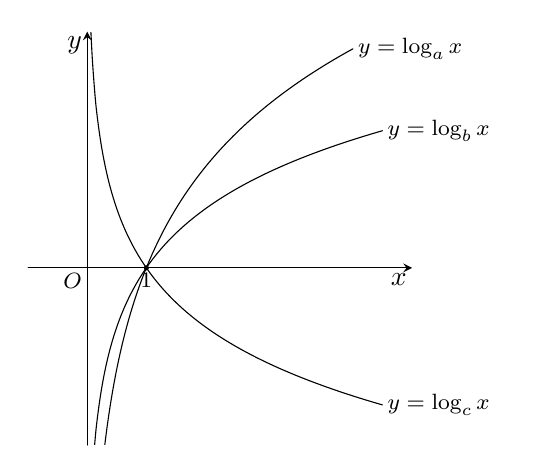
\begin{tikzpicture}[line join=round,line cap=round,>=stealth,scale=0.75,font=\footnotesize]
			\tikzset{every node/.style={outer sep=-0.5mm}}
			\def \xmin{-1} \def \xmax{7.5}
			\def \ymin{-3} \def \ymax{4}
			\def \fx{ln(\x)/ln(2)}
			\def \gx{ln(\x)/ln(0.5)}
			\def \hx{ln(\x)/ln(1.5)}
			\draw[->] (\xmin,0)--(5.5,0) node[below left] {\normalsize$x$};
			\draw[->] (0,\ymin)--(0,\ymax) node[below left] {\normalsize$y$};
			\draw (0,0) node[below left] {$O$};
			\foreach \x in {1} \fill (\x,0) circle (1.25pt) node[below] {$\x$};
			\begin{scope}
				\clip (\xmin+0.01,\ymin+0.01) rectangle (\xmax-0.01,\ymax-0.01);
				\draw[samples=150,domain=0.01:5,smooth,variable=\x] plot (\x,{\fx}) node[right]{$y=\log_bx$};
				\draw[samples=150,domain=0.01:5,smooth,variable=\x] plot (\x,{\gx})node[right]{$y=\log_cx$};
				\draw[samples=150,domain=0.01:4.5,smooth,variable=\x] plot (\x,{\hx})node[right]{$y=\log_ax$};
			\end{scope}
		\end{tikzpicture}
	\end{center}
	\choiceTF
	{Hàm số $y=\log_cx$ đồng biến trên khoảng $(0;+\infty)$}
	{Đường thẳng $ y=3$ cắt hai đồ thị $y=\log_ax$, $y=\log_bx$ tại các điểm có hoành độ lần lượt là $x_1$, $x_2$ sao cho $x_2=2x_1$. Khi đó $\dfrac{a}{b}=\sqrt[3]{2}$}
	{\True Từ đồ thị ta có $ 0<c<1<a<b$}
	{\True Đồ thị các hàm số trên đều đi qua điểm $ A(1;0)$}
	\loigiai{
		\begin{itemchoice}
			\itemch Hàm số $y=\log_cx$ nghịch biến trên khoảng $(0;+\infty)$.
			\itemch Giả sử đường thẳng $ y=3$ cắt hai đồ thị hàm số $y=\log_ax$, $y=\log_bx$ tại các điểm $ A(x_1;3)$, $B(x_2;3)$.\\
			Khi đó, $\log_ax_1=3\Leftrightarrow x_1=a^3$; $\log_b x_2=3\Leftrightarrow x_2=b^3$.\\
			Theo giả thiết, ta có $x_2=2x_1\Leftrightarrow b^3=2a^3\Leftrightarrow\dfrac{b^3}{a^3}=2\Leftrightarrow\dfrac{b}{a}=\sqrt[3]{2}$.
			\itemch 
			Hàm số $y=\log_cx$ nghịch biến trên khoảng $(0;+\infty)\Rightarrow 0<c<1$.\\
			Hàm số $y=\log_ax$, $y=\log_bx$ đồng biến trên khoảng $(0;+\infty)\Rightarrow a>1$, $b>1$.\\
			Vẽ đường thẳng $y=1$ cắt hai đồ thị $y=\log_ax$, $y=\log_bx$ tại các điểm $M$, $N$. Khi đó $x_M=a$, $x_N=b$. Từ hình vẽ ta có $1<a<b$.\\
			Vậy $0<c<1<a<b$.
			\itemch 
			Đồ thị các hàm số trên đều đi qua điểm $A(1;0)$.
		\end{itemchoice}
	}
\end{ex}

\begin{ex}%[1D7H2-1]%[Dự án C đề thi thử TN Môn Toán NH25-26 - Dot 4 - Trần Xuân Hoa]%[THPT Mai Anh Tuấn - Thanh Hóa]%[GVPB - Lê Hữu Kiệt]
	Cho hàm số $f(x) = 2 \cos x - x + \pi + 2\,026$.
	\choiceTF
	{\True $f(\pi) = 2\,024$}
	{Đạo hàm của hàm số đã cho là $f'(x) = 2 \sin x - 1$}
	{Số nghiệm của phương trình $f'(x) = 0$ trên đoạn $\left[-\dfrac{\pi}{2}; \dfrac{\pi}{2}\right]$ là $2$}
	{\True Giá trị nhỏ nhất của $f(x)$ trên đoạn $\left[-\dfrac{\pi}{2}; \dfrac{\pi}{2}\right]$ là $\dfrac{\pi}{2} + 2\,026$}
	\loigiai{
		\begin{itemchoice}
			\itemch Ta có $f(\pi) = 2 \cos \pi - \pi + \pi + 2026 = 2\cdot (-1) + 2\,026 = -2 + 2\,026 = 2\,024$.
			\itemch Ta có $f'(x) = -2 \sin x - 1$.
			\itemch Ta có $f'(x) = 0 \Leftrightarrow \sin x = -\dfrac{1}{2} \Leftrightarrow \hoac{&x=-\dfrac{\pi}{6}+k2\pi\\&x=\dfrac{7\pi}{6}+k2\pi.}$\\
			Xét
			\begin{itemize}
				\item $-\dfrac{\pi}{2}\le \dfrac{7\pi}{6}+k2\pi\le \dfrac{\pi}{2}\Leftrightarrow k\in \varnothing$.
				\item $-\dfrac{\pi}{2}\le -\dfrac{\pi}{6}+k2\pi\le \dfrac{\pi}{2}\Leftrightarrow k\in \{0\}$.  phương trình có $1$ nghiệm $x=-\dfrac{\pi}{6}$.
			\end{itemize}
			\itemch Ta có $f\left(-\dfrac{\pi}{2}\right) = \dfrac{3\pi}{2} + 2\,026$, $ f\left(\dfrac{\pi}{2}\right) = \dfrac{\pi}{2} + 2\,026$, $f\left(-\dfrac{\pi}{6}\right) = \dfrac{7\pi}{6} + 2\,026 + \sqrt{3}$.\\
			Do đó, giá trị nhỏ nhất của $f(x)$ trên đoạn $\left[-\dfrac{\pi}{2}; \dfrac{\pi}{2}\right]$ là $\dfrac{\pi}{2} + 2\,026$.
		\end{itemchoice}
	}
\end{ex}

\begin{ex}%[1D7V1-5]%[Dự án C đề thi thử TN Môn Toán NH25-26 - Dot 4 - BCTuan]%[THPT Nguyễn Trãi-Hà Nội]%[GVPB-Khắc Thiên]
	Mực nước $h$ (đơn vị: mét) tại một cảng biển sau $t$ giờ tính từ thời điểm nửa đêm được xác định bởi công thức $h(t)=4\cos\left(\dfrac{\pi t}{6}+\dfrac{\pi}{3}\right)+10$ với ($0 \le t \le 24$).
	\choiceTF
	{Tại thời điểm nửa đêm $t=0$, mực nước tại cảng là $15$ mét}
	{\True Tốc độ biến thiên của mực nước tại thời điểm $t$ là $h'(t)=-\dfrac{2\pi}{3}\sin\left(\dfrac{\pi t}{6}+\dfrac{\pi}{3}\right)$}
	{\True Trong một ngày (với $0 \le t \le 24$), mực nước thấp nhất là $6$ mét và mực nước này xuất hiện tại hai thời điểm khác nhau}
	{\True Phương trình $h'(t)=0$ có một nghiệm trên đoạn $[0;6]$ là $t=4$}
	\loigiai{
		\begin{itemchoice}
			\itemch Tại thời điểm $t=0$, mực nước là $h(0) = 4\cos\left(\dfrac{\pi}{3}\right)+10 = 4 \cdot \dfrac{1}{2} + 10 = 12$ (mét). 			
			\itemch Tốc độ biến thiên của mực nước là đạo hàm của hàm số $h(t)$ là
			\[h'(t) = 4 \cdot \left(\dfrac{\pi}{6}\right) \cdot \left[-\sin\left(\dfrac{\pi t}{6}+\dfrac{\pi}{3}\right)\right] = -\dfrac{2\pi}{3}\sin\left(\dfrac{\pi t}{6}+\dfrac{\pi}{3}\right).\]			
			\itemch Ta có $\cos\left(\dfrac{\pi t}{6}+\dfrac{\pi}{3}\right) \ge -1$, suy ra $h(t) \ge 4(-1)+10 = 6$.\\
			Mực nước thấp nhất là $6$ mét.\\
			Dấu đẳng thức xảy ra khi
			\begin{eqnarray*}
				&& \cos\left(\dfrac{\pi t}{6}+\dfrac{\pi}{3}\right) = -1\\
				& \Leftrightarrow& \dfrac{\pi t}{6}+\dfrac{\pi}{3} = \pi + k2\pi\\
				& \Leftrightarrow& \dfrac{t}{6} = \dfrac{2}{3} + 2k\\
				& \Leftrightarrow& t = 4 + 12k \quad (k\in \mathbb{Z}).
			\end{eqnarray*}
			Vì $0 \le t \le 24$ nên $0 \le 4+12k \le 24 \Leftrightarrow -\dfrac{1}{3} \le k \le \dfrac{5}{3}$.\\
			Vì $k \in \mathbb{Z}$ nên $k \in \{0; 1\}$.\\ 
			Khi đó $t = 4$ hoặc $t = 16$.\\
			Vậy mực nước thấp nhất xuất hiện tại hai thời điểm khác nhau.			
			\itemch Xét phương trình
			\begin{eqnarray*}
				h'(t) = 0
				& \Leftrightarrow& -\dfrac{2\pi}{3}\sin\left(\dfrac{\pi t}{6}+\dfrac{\pi}{3}\right) = 0\\
				& \Leftrightarrow& \sin\left(\dfrac{\pi t}{6}+\dfrac{\pi}{3}\right) = 0\\
				& \Leftrightarrow& \dfrac{\pi t}{6}+\dfrac{\pi}{3} = k\pi\\
				& \Leftrightarrow& t = 6k - 2 \,\, (k\in \mathbb{Z}).
			\end{eqnarray*}
			Với $t\in [0;6]$ ta có
			\[0 \le 6k-2 \le 6 \Leftrightarrow \dfrac{1}{3} \le k \le \dfrac{4}{3}.\]
			Vì $k \in \mathbb{Z}$ nên $k=1$ suy ra $t=4$.\\
			Vậy phương trình có một nghiệm duy nhất $t=4$ trên đoạn $[0;6]$.
		\end{itemchoice}
	}
\end{ex}

\begin{ex}%[1D9H1-3]%[Dự án đề thi thử NH25-26]%[THPT Chuyên Phan Bội Châu - Nghệ An]%[Thanh Ta]
	\lq\lq Cú nhảy tử thần\rq\rq\ của ngỗng Barnacle ở Bắc Cực là một trong những hình ảnh ấn tượng và tạo ra nhiều cảm xúc nhất trong thế giới tự nhiên. Vào mùa sinh sản, để tránh kẻ thù ngỗng bố mẹ sẽ làm tổ trên vách đá cao hơn $100$ (m). Khi ngỗng con ra đời được vài ngày thì phải cùng ngỗng bố mẹ nhảy từ vách đá xuống mặt đất để kiếm ăn. Nhờ bản năng sinh tồn cùng với lớp lông vũ bảo vệ mà tỉ lệ sống sót của ngỗng con khi thực hiện \lq\lq Cú nhảy tử thần\rq\rq\ rất cao, ngỗng con đực là $80\%$ và ngỗng con cái là $90\%$. Hôm nay, ngỗng bố mẹ sẽ dìu dắt $3$ ngỗng con gồm một con đực và hai con cái thực hiện cú nhảy đầu đời ngoạn mục này.
	\choiceTF
	{\True Xác suất để cả $3$ ngỗng con sống sót sau \lq\lq Cú nhảy tử thần\rq\rq\ là $0{,}648$}
	{Xác suất để cả $3$ ngỗng con tử vong sau \lq\lq Cú nhảy tử thần\rq\rq\ là $0{,}02$}
	{\True Xác suất để ít nhất $1$ ngỗng con sống sót sau \lq\lq Cú nhảy tử thần\rq\rq\ là $0{,}998$}
	{\True Xác suất để có đúng $2$ ngỗng con sống sót sau \lq\lq Cú nhảy tử thần\rq\rq\ là $0{,}306$}
	\loigiai{
		Gọi $A$ là biến cố ngỗng con đực sống sót, $B_1$ và $B_2$ lần lượt là biến cố hai ngỗng con cái sống sót.
		Theo giả thiết, ta có xác suất của các biến cố thành phần như sau:
		\begin{itemize}
			\item $\mathrm{P}(A) = 80\% = 0{,}8 \Rightarrow \mathrm{P}\left(\overline{A}\right) = 1 - 0{,}8 = 0{,}2$.
			\item $\mathrm{P}(B_1) = 90\% = 0{,}9 \Rightarrow \mathrm{P}\left(\overline{B_1}\right) = 1 - 0{,}9 = 0{,}1$.
			\item $\mathrm{P}(B_2) = 90\% = 0{,}9 \Rightarrow \mathrm{P}\left(\overline{B_2}\right) = 1 - 0{,}9 = 0{,}1$.
		\end{itemize}
		\begin{itemchoice}
			\itemch Gọi $X$ là biến cố cả $3$ con sống sót: $X = A \cap B_1 \cap B_2$.\\
			Vì khả năng sống sót của mỗi con là độc lập, ta có
			\[\mathrm{P}(X) = \mathrm{P}(A) \cdot \mathrm{P}(B_1) \cdot \mathrm{P}(B_2) = 0{,}8 \cdot 0{,}9 \cdot 0{,}9 = 0{,}648.\]
			\itemch Gọi $Y$ là biến cố cả $3$ con tử vong: $Y = \overline{A} \cap \overline{B_1} \cap \overline{B_2}$.\\
			Ta có
			\[\mathrm{P}(Y) = \mathrm{P}\left(\overline{A}\right) \cdot \mathrm{P}\left(\overline{B_1}\right) \cdot \mathrm{P}\left(\overline{B_2}\right) = 0{,}2 \cdot 0{,}1 \cdot 0{,}1 = 0{,}002 \neq 0{,}02.\]
			\itemch Gọi $Z$ là biến cố có ít nhất $1$ con sống sót. Biến cố đối của $Z$ chính là biến cố cả $3$ con đều tử vong ($Y$).\\
			Ta có
			\[\mathrm{P}(Z) = 1 - \mathrm{P}(Y) = 1 - 0{,}002 = 0{,}998.\]
			\itemch Có $3$ trường hợp xảy ra để có đúng $2$ con sống sót:
			\begin{itemize}
				\item Con đực sống, con cái $1$ sống, con cái $2$ chết: $0{,}8 \cdot 0{,}9 \cdot 0{,}1 = 0{,}072$.
				\item Con đực sống, con cái $1$ chết, con cái $2$ sống: $0{,}8 \cdot 0{,}1 \cdot 0{,}9 = 0{,}072$.
				\item Con đực chết, con cái $1$ sống, con cái $2$ sống: $0{,}2 \cdot 0{,}9 \cdot 0{,}9 = 0{,}162$.
			\end{itemize}
			Tổng xác suất là
			\[\mathrm{P}(\text{đúng hai con ngỗng sống}) = 0{,}072 + 0{,}072 + 0{,}162 = 0{,}306.\]
		\end{itemchoice}
	}
\end{ex}

\begin{ex}%[Đề thi thử môn Toán TRƯỜNG THPT Cổ Loa TỈNH Hà Nội năm học 2025-2026]%[Lâm Xương Thăng - Lê Phúc]%[1D9H2-4]
	Một trường học có $2\,000$ học sinh. Trong đó có $1\,000$ học sinh thích bóng đá, $1\,400$ học sinh thích bóng rổ và $800$ học sinh thích cả hai môn này. Chọn ngẫu nhiên một học sinh trong trường.
	\choiceTF
	{\True Xác suất để học sinh được chọn thích bóng đá là $0{,}5$}
	{Xác suất để học sinh được chọn không thích bóng rổ là $0{,}7$}
	{\True Xác suất để học sinh được chọn thích cả bóng đá và bóng rổ là $0{,}4$}
	{\True Xác suất để học sinh được chọn thích ít nhất một môn là $0{,}8$}
	\loigiai{
		Gọi $A$ là tập hợp học sinh thích bóng đá, $B$ là tập hợp học sinh thích bóng rổ.\\
		Khi đó $A \cap B$ là tập hợp học sinh thích cả hai môn này, $A \cup B$ là tập hợp học sinh thích ít nhất một trong hai môn này.\\
		Ta có $n(A \cup B) = n(A) + n(B) - n(A \cap B) = 1\,000 + 1\,400 - 800 = 1\,600$.
		\begin{itemchoice}
			\itemch Xác suất để học sinh được chọn thích bóng đá là $\mathrm{P}(A) = \dfrac{1\,000}{2\,000} = 0{,}5$.
			
			\itemch Xác suất để học sinh được chọn không thích bóng rổ là 
			\[\mathrm{P}\left(\overline{B}\right) = 1 - \mathrm{P}(B) = 1 - \dfrac{1\,400}{2\,000} = 1 - \dfrac{7}{10} = \dfrac{3}{10} = 0{,}3.\]
			\itemch Xác suất để học sinh được chọn thích cả bóng đá và bóng rổ là 
			\[\mathrm{P}(A \cap B) = \dfrac{800}{2\,000} = 0{,}4.\]
			\itemch Xác suất để học sinh được chọn thích ít nhất một môn là 
			\[\mathrm{P}(A \cup B) = \dfrac{1\,600}{2\,000} = 0{,}8.\]
		\end{itemchoice}
	}
\end{ex}

\begin{ex}%[1D9V1-3]%[Dự án C đề thi thử TN Môn Toán NH25-26 - Dot 4 - Võ Thị Thùy Trang]%[Liên trường THPT cụm 09 - Đợt 2 - Hà Nội]%[GVPB - Thanh Phát]
	Hộp thứ nhất có $8$ viên bi gồm màu xanh và màu đỏ, hộp thứ hai có $2$ viên bi màu xanh và một số viên bi màu đỏ. Chọn ngẫu nhiên từ mỗi hộp $2$ viên bi. Gọi $A$ là biến cố \lq\lq Chọn được $2$ viên bi màu xanh ở hộp thứ nhất\rq\rq\ và $B$ là biến cố \lq\lq Chọn được $2$ viên bi màu xanh ở hộp thứ hai\rq\rq. Biết $\mathrm{P}(A)=\dfrac{3}{28}$ và $\mathrm{P}(B)=\dfrac{1}{15}$.
	\choiceTF
	{\True $A$ và $B$ là $2$ biến cố độc lập với nhau}
	{\True Xác suất để đồng thời cả hai hộp đều lấy được $2$ viên bi màu xanh bằng $\dfrac{1}{140}$}
	{\True Xác suất để chọn được ít nhất $1$ viên bi màu đỏ ở hộp thứ nhất bằng $\dfrac{25}{28}$}
	{Tổng số viên bi màu đỏ ở hai hộp bằng $8$}
	\loigiai{
		\begin{itemchoice}
			\itemch Dựa vào đề bài đã cho ta có $A$ và $B$ là $2$ biến cố độc lập với nhau.
			\itemch $AB$ là biến cố \lq\lq Cả hai hộp đều lấy được $2$ viên bi xanh\rq\rq.\\
			Do $A$ và $B$ là $2$ biến cố độc lập với nhau nên $\mathrm{P}(AB)=\mathrm{P}(A)\cdot \mathrm{P}(B)=\dfrac{1}{140}$.
			\itemch $A$ là biến cố \lq\lq Chọn được $2$ viên bi màu xanh ở hộp thứ nhất\rq\rq\\
			Suy ra $\overline{A}$ là biến cố \lq\lq Chọn được ít nhất $1$ viên bi màu đỏ ở hộp thứ nhất\rq\rq.\\
			Xác suất cần tìm là $\mathrm{P}\left(\overline{A}\right)=1-\mathrm{P}(A)=1-\dfrac{3}{28}=\dfrac{25}{28}$.
			\itemch 
			\begin{itemize}
				\item Giả sử ở hộp thứ nhất có $x$ viên bi xanh, điều kiện $2<x<8$ và $x\in\mathbb{N}^*$.\\
				Phép thử \lq\lq chọn $2$ viên bi từ hộp thứ nhất\rq\rq.\\
				Ta có $n(\Omega)=\mathrm{C}_8^2$ và $n(A)=\mathrm{C}_x^2=\dfrac{x!}{2!(x-2)!}=\dfrac{x(x-1)}{2}$.\\
				Mặt khác $\mathrm{P}(A)=\dfrac{3}{28} \Leftrightarrow \dfrac{x(x-1)}{56}=\dfrac{3}{28} \Leftrightarrow \hoac{&x=3&&\text{(nhận)}\\&x=-2&&\text{(loại)}.}$\\
				Do đó trong hộp thứ nhất có $3$ viên bi màu xanh và $5$ viên bi màu đỏ.
				\item Giả sử ở hộp thứ hai có $y$ viên bi, điều kiện $y>2$ và $y\in\mathbb{N}$.\\
				Phép thử \lq\lq chọn $2$ viên bi từ hộp thứ hai\rq\rq.\\
				Ta có $n(\Omega)=\mathrm{C}_y^2=\dfrac{y(y-1)}{2}$ và $n(B)=\mathrm{C}_2^2=1$.\\
				Mặt khác $\mathrm{P}(B)=\dfrac{1}{15} \Leftrightarrow \dfrac{2}{y(y-1)}=\dfrac{1}{15} \Leftrightarrow \hoac{&y=6&&\text{(nhận)}\\&y=-5&&\text{(loại).}}$\\
				Do đó trong hộp thứ hai có $2$ viên bi màu xanh và $4$ viên bi màu đỏ.
			\end{itemize}
			Tổng số bi đỏ ở cả $2$ hộp là $9$.
		\end{itemchoice}
	}
\end{ex}

\begin{ex}%[1H8V5-4]%[Dự án đề TT-THPT-TranNhanTong-HaNoi-N25-26-Dot 3- Nguyễn Văn Nghĩa]%[SGD Hà Nội] %[GVPB - Phan Quốc Trí]
	Cho hình chóp $S.ABCD$ có đáy $ABCD$ là hình chữ nhật, $SA \perp (ABCD)$. Biết $SA = 2$; $AB = \sqrt{2}$; $AC = \sqrt{3}$.
	\choiceTF
	{\True $AD \parallel (SBC)$}
	{Khoảng cách từ $D$ đến mặt phẳng $(SBC)$ là $\dfrac{\sqrt{3}}{3}$}
	{$\tan$ của góc giữa $SC$ và mặt phẳng $(ABCD)$ là $\dfrac{\sqrt{3}}{2}$}
	{\True Khoảng cách giữa $2$ đường thẳng $SD$ và $AB$ là $\dfrac{2\sqrt{5}}{5}$}
	\loigiai{
\begin{center}
	\begin{tikzpicture}[scale=1,font=\footnotesize,line join=round
		,line cap=round,>=stealth]
	\def\a{4}
	\def\h{4}
	\path 	(0:0) coordinate (A)
			++(0:\a) coordinate (D)
			++(-130:\a/2) coordinate (C)
			($(A)+(C)-(D)$) coordinate (B)
			($(A)+(90:\h)$) coordinate (S)
			($(B)!(A)!(S)$) coordinate (H)
			($(D)!(A)!(S)$) coordinate (K)
			(intersection of A--C and B--D) coordinate (O);%giao điểm O
	\draw[dashed,thick] 	(H)--(A)--(K) (B)--(A)--(D)	(C)--(A)--(S);
	\draw[thick] 			(B)-- (C)--(D)
			(B)--(S)	(C)--(S)	(D)--(S);
	\foreach \x/\g in {A/-90,B/-135,C/-45,D/45,S/90,H/150,K/30}
			\fill[black] 	(\x) circle (1.5pt)
			($(\g:3mm)+(\x)$) node {$\x$};	
	\draw pic[draw,angle radius=3mm]{right angle=D--A--S};
	\draw pic[draw,angle radius=3mm]{right angle=D--K--A};
	\draw pic[draw,angle radius=3mm]{right angle=B--H--A};%Theo chiều dương	
\end{tikzpicture}
\end{center}
		\begin{itemchoice}
			\itemch 
			Vì $AD \parallel BC$ và $BC \subset (SBC)$ nên $AD \parallel (SBC)$.
			\itemch 
			Vì $AD \parallel (SBC)$ suy ra $\mathrm{d}(D,(SBC)) = \mathrm{d}(A,(SBC))$.\\
			Trong $\triangle SAB$ kẻ $AH \perp SB$.\\ 
			Ta có $\heva{&BC\perp AB\\&BC\perp SA}\Rightarrow BC\perp (SAB)\Rightarrow BC\perp AH$.\\
			Suy ra $AH\perp(SBC)$.\\
			Suy ra $\mathrm{d}(D,(SBC)) = \mathrm{d}(A,(SBC))=AH$.\\
			Xét $\triangle SAB$, vuông tại $A$ có $AH$ là đường cao nên
			$$AH = \dfrac{SA \cdot AB}{\sqrt{SA^2 + AB^2}} = \dfrac{2 \cdot \sqrt{2}}{\sqrt{4 + 2}} = \dfrac{2\sqrt{2}}{\sqrt{6}} = \dfrac{2\sqrt{3}}{3}.$$
			\itemch 
			Ta có $AC$ là hình chiếu của $SC$ trên $(ABCD)$ nên góc giữa $SC$ và $(ABCD)$ là $\widehat{SCA} $.\\
			Trong $\triangle SAC$ vuông tại $A$, ta có $\tan \widehat{SCA} = \dfrac{SA}{AC} = \dfrac{2}{\sqrt{3}} = \dfrac{2\sqrt{3}}{3}$.
			\itemch 
			Vì $AB \parallel CD$ nên $AB \parallel (SCD)$ suy ra $\mathrm{d}(AB, SD) = \mathrm{d}(AB, (SCD)) = \mathrm{d}(A, (SCD))$.\\
			Trong $\triangle SAD$ kẻ $AK \perp SD$ .\\
			Ta có $\heva{&CD\perp AD\\&CD\perp SA}\Rightarrow CD\perp(SAD)\Rightarrow CD\perp AK$.\\
			Suy ra $AK\perp(SCD)$.\\
			Xét $\triangle ABC$, 
			ta có $BC = \sqrt{AC^2 - AB^2} = \sqrt{3 - 2} = 1$ suy ra $AD = 1$.\\
			Xét $\triangle SAD$ vuông tại $A$ có $AK$ là đường cao nên $$AK = \dfrac{SA \cdot AD}{\sqrt{SA^2 + AD^2}} = \dfrac{2 \cdot 1}{\sqrt{4 + 1}} = \dfrac{2}{\sqrt{5}} = \dfrac{2\sqrt{5}}{5}.$$
		\end{itemchoice}
	}
\end{ex}

\begin{ex}%[1H8V7-4]%%[Dự án đề TT Toán NH25-26-Dot3-Đắc Vũ]%[Cụm 13-Hải Phòng]%[GVPB-Viet Hoang Pham]
	\immini{
		Cho hình lăng trụ $ABC.A'B'C'$ có tam giác $ABC$ vuông cân tại $A$, hình chiếu vuông góc của $A'$ trên mặt phẳng $(ABC)$ trùng với trọng tâm $H$ của tam giác $ABC$. Biết $AA' = BC = a\sqrt{2}$.
		\choiceTF
		{Thể tích khối lăng trụ đã cho bằng $\dfrac{2a^3}{9}$}
		{\True Độ dài đường cao hình lăng trụ bằng $\dfrac{4a}{3}$}
		{\True Khoảng cách giữa hai đường thẳng $BB'$ và $AC$ gấp ba lần khoảng cách từ $H$ đến mặt phẳng $(ACC'A')$}
		{Khoảng cách giữa hai đường thẳng $BB'$ và $AC$ bằng $\dfrac{4a\sqrt{17}}{51}$}}{\begin{tikzpicture}[font=\footnotesize, line join=round,line cap=round, >=stealth,thick,scale=0.7]
			\tikzset{every node/.style={scale=0.9}}
			\path 
			(0,0) coordinate (A)
			(6,0) coordinate (C)
			(-45:3) coordinate (B)
			($(B)!.5!(C)$) coordinate (M)
			($(A)!2/3!(M)$) coordinate (H)
			(H)+(90:4) coordinate (A')
			($(A')+(B)$) coordinate (B')
			($(A')+(C)$) coordinate (C')
			($(A)!1/3!(B)$) coordinate (K)
			($(A')!3/5!(K)$) coordinate (I)
			;
			\draw (A')--(B')--(C')--cycle (B)--(B') (C)--(C') (A)--(B)--(C) (A)--(A')--(K);
			\draw[dashed,thin](M)--(A)--(C) (A')--(H)--(K) (H)--(I);
			\foreach \i/\g  in {A/180,B/-90,C/0,A'/90,B'/90,C'/90,K/180,I/180,M/-90,H/-90} \fill[black] (\i) circle(1pt)+(\g:0.5) node{$\i$}; 
	\end{tikzpicture}}
	\loigiai{
		\begin{itemchoice}
			\itemch 
			
			Ta có $AM = \dfrac{1}{2}BC = \dfrac{a\sqrt{2}}{2}; AH = \dfrac{2}{3}AM = \dfrac{a\sqrt{2}}{3} \Rightarrow A'H = \sqrt{AA'^2 - AH^2} = \dfrac{4a}{3}$.\\
			Do $AB = AC = a \Rightarrow S_{\Delta ABC} = \dfrac{1}{2}AB^2 = \dfrac{a^2}{2} \Rightarrow V_{ABC.A'B'C'} = \dfrac{2a^3}{3}$.
			\itemch 
			
			Ta có $AM = \dfrac{1}{2}BC = \dfrac{a\sqrt{2}}{2}; AH = \dfrac{2}{3}AM = \dfrac{a\sqrt{2}}{3} \Rightarrow A'H = \sqrt{AA'^2 - AH^2} = \dfrac{4a}{3}$.
			
			\itemch 
			
			Do $BB' \parallel (ACC'A')$ nên $\mathrm{d}(BB';AC) = \mathrm{d}(BB',(ACC'A')) = \mathrm{d}(B,(ACC'A'))$.\\
			Ta có $\dfrac{\mathrm{d}(B,(ACC'A'))}{\mathrm{d}(H,(ACC'A'))} = \dfrac{BN}{HN} = 3$.
			\\ 
			Suy ra $\mathrm{d}(BB';AC) = 3 \cdot \mathrm{d}(H,(ACC'A'))$.
			
			\itemch 
			
			Kẻ $HK \perp AC$ và $HI \perp A'K$. Khi đó $HI \perp (ACC'A') \Rightarrow \mathrm{d}(H,(ACC'A')) = HI$.\\
			Ta có $HK \parallel AB \Rightarrow \dfrac{HK}{AB} = \dfrac{NH}{NB} = \dfrac{1}{3} \Rightarrow HK = \dfrac{1}{3}AB = \dfrac{a}{3}$.\\
			$\mathrm{d}(BB',AC) = 3 \cdot \mathrm{d}(H,(ACC'A')) = 3 \cdot HI = 3 \cdot \dfrac{A'H \cdot HK}{\sqrt{A'H^2 + HK^2}} = \dfrac{4a}{\sqrt{17}} = \dfrac{4\sqrt{17}a}{17}$.
		\end{itemchoice}
	}
\end{ex}

\begin{ex}%[2D1C5-6]%[Dự án C đề thi thử tót nghiệp TN môn Toán NH25-26-Đợt 4- Nguyễn Văn Nghĩa] %[Trường-THPT-LeQuyDon-DongDa-HaNoi--NH25-26]%[GVPB - Phan Quốc Trí]
	Cho hàm số $y = \dfrac{2x^2 - 5x + 7}{x - 5}$ có đồ thị $(C)$.
	\choiceTF
	{\True Tổng tất cả các giá trị cực trị của hàm số bằng $30$}
	{Hàm số nghịch biến trên khoảng $(-1; 5)$}
	{Đường tiệm cận xiên của đồ thị $(C)$ có phương trình $y = 2x - 5$}
	{Tiếp tuyến của $(C)$ tại điểm $M(3; -5)$ cắt các đường tiệm cận đứng và tiệm cận xiên lần lượt tại $P$, $Q$. Diện tích tam giác $OPQ$ là $52$, với $O$ là gốc tọa độ}
	\loigiai{
		Tập xác định là $\mathscr{D}=\mathbb{R}\setminus \left\lbrace 5\right\rbrace $.\\
		Ta có $\dfrac{2x^2 - 5x + 7}{x - 5} = 2x + 5 + \dfrac{32}{x - 5}$.\\
		Suy ra $\lim\limits_{x\rightarrow+\infty}\left[y-(2x+5)\right] =\lim\limits_{x\rightarrow+\infty}\dfrac{32}{x-5}=0$.\\
		$\lim\limits_{x\rightarrow-\infty}\left[y-(2x+5)\right]=\lim\limits_{x\rightarrow-\infty}\dfrac{32}{x-5}=0$.\\
		Suy ra đồ thị hàm số có tiệm cận xiên $y = 2x + 5$.\\
		Ta có $\lim\limits_{x\rightarrow 5^+}\dfrac{2x^2 - 5x + 7}{x - 5}=+\infty$ và $\lim\limits_{x\rightarrow 5^-}\dfrac{2x^2 - 5x + 7}{x - 5}=-\infty$.\\
		Suy ra đồ thị hàm số có tiệm cận đứng $x = 5$.\\
		Ta có
		$y' = \dfrac{(4x - 5)(x - 5) - (2x^2 - 5x + 7)}{(x - 5)^2} = \dfrac{2x^2 - 20x + 18}{(x - 5)^2}$. \\
		$y' = 0 \Leftrightarrow 2x^2 - 20x + 18 = 0 \Leftrightarrow \hoac{&x=1\\& x=9}\Rightarrow \hoac{&y=-1\\&y=31.} $\\ 
		Ta có bảng biến thiên như sau
		\begin{center}
			
\begin{tikzpicture}
				\tkzTabInit[nocadre=false,lgt=1.2,espcl=2.5,deltacl=0.6]
				{$x$ /1, $y'$ /1, $y$ /2} 
				{$-\infty$, $1$, $5$, $9$, $+\infty$} 
				\tkzTabLine{, +, 0, -, d, -, 0, +, }
				\tkzTabVar{
					-/ $-\infty$, 
					+/{$-1$}, 
					-D+/ $-\infty$ / $+\infty$, 
					-/ {$31$}, 
					+/ $+\infty$
				}
			\end{tikzpicture}
		\end{center}
		\begin{itemchoice}
			\itemch  
			Dựa vào bảng biến thiên ta có tổng giá trị cực đại và cực tiểu là $-1 + 31 = 30$.
			\itemch Dựa vào bảng biến thiên ta thấy hàm số nghịch biến trên $(1; 5)$ và $(5; 9)$.
			\itemch Đường tiệm cận xiên của đồ thị hàm số là $y = 2x + 5$.
			\itemch 
			$y'(3) = \dfrac{2\cdot 9 - 60 + 18}{4} = -6$. \\
			Phương trình tiếp tuyến $(d)$ của $(C)$ tại điểm $M(3; -5)$ là $$y + 5 = -6(x - 3)\Leftrightarrow y = -6x + 13.$$
			Giao điểm của $(d)$ với tiệm cận đứng $x = 5 \Rightarrow y = -6 \cdot 5 + 13 = -17$ ta được $P(5;-17)$ \\
			Giao với tiệm cận xiên $-6x + 13 = 2x + 5 \Leftrightarrow x = 1 \Rightarrow y = 7$ ta được $Q(1; 7)$ \\
			Diện tích tam giác $OPQ$ là $S = \dfrac{1}{2} \left| 5 \cdot 7 - (-17) \cdot 1\right|= 26$.
		\end{itemchoice}
	}
\end{ex}

\begin{ex}%[Đề thi thử môn Toán TRƯỜNG THPT Cổ Loa TỈNH Hà Nội năm học 2025-2026]%[Lâm Xương Thăng - Lê Phúc]%[2D1H2-1]
	Cho hàm số $f(x) = x^3 - 3x$.
	\choiceTF
	{Hàm số đã cho có đạo hàm là $f'(x) = 3x^2 + 3$}
	{$f'(x) < 0$ khi $x \in (-\infty; -1) \cup (1; +\infty)$ và $f'(x) > 0$ khi $x \in (-1; 1)$}
	{\True Hàm số đã cho nghịch biến trên khoảng $(-1; 1)$}
	{\True Giá trị cực tiểu hàm số đã cho là $-2$}
	\loigiai{
		\begin{itemchoice}
			\itemch Hàm số đã cho có đạo hàm là $f'(x) = 3x^2 - 3$.
			
			\itemch Ta có $f'(x) = 0 \Leftrightarrow 3x^2 - 3 = 0 \Leftrightarrow \hoac{&x = 1 \\ &x = -1.}$\\
			Hàm số đã cho có bảng biến thiên
			\begin{center}
				
\begin{tikzpicture}
					\tkzTabInit[nocadre=false,lgt=1.2,espcl=3]
					{$x$ /0.6, $f'(x)$ /0.6, $f(x)$ /2}
					{$-\infty$, $-1$, $1$, $+\infty$}
					\tkzTabLine{ , + , 0 , - , 0 , + , }
					\tkzTabVar{-/ $-\infty$, +/ $2$, -/ $-2$, +/ $+\infty$}
				\end{tikzpicture}
			\end{center}
			Từ bảng biến thiên ta có 
			\begin{itemize}
				\item $f'(x) < 0$ khi $x \in (-1; 1)$.
				\item $f'(x) > 0$ khi $x \in (-\infty; -1) \cup (1; +\infty)$.
			\end{itemize}
			
			\itemch Từ bảng biến thiên suy ra hàm số đã cho nghịch biến trên khoảng $(-1; 1)$.
			
			\itemch Từ bảng biến thiên suy ra giá trị cực tiểu hàm số đã cho là $-2$.
		\end{itemchoice}
	}
\end{ex}

\begin{ex}%[2D1H2-1]%[Dự án C đề thi thử TN Môn Toán NH25-26 - Dot 4 - Quốc Dũng]%[ Trường THPT Nguyễn Trung Thiên - Hà Tĩnh]%[GVPB - Phan Anh]		
	Cho hàm số $y=-x^3+3x^2+4$ có đồ thị $\left(C\right)$
	\choiceTF
	{\True Hàm số có đạo hàm $y'=-3x^2+6x$}
	{\True Hàm số đồng biến trên khoảng $\left(0;2\right)$}
	{Đồ thị có hai điểm cực trị và đường thẳng đi qua hai điểm cực trị là $2x+y-4=0$}
	{\True Diện tích $\Delta AOB$ bằng 4 trong đó $A$ và $B$ là hai điểm cực trị của đồ thị $\left(C\right)$}
	\loigiai{
		\begin{itemchoice}
			\itemch 
			Ta có $y=-x^3+3x^2+4\Rightarrow y'=-3x^2+6x$.
			\itemch 
			Ta có $y'=-3x^2+6x$. Cho $y'=0\Leftrightarrow -3x^2+6x=0\Leftrightarrow
			\hoac{& x=0 \\ 	& x=2.}$\\
			Bảng biến thiên
			\begin{center}
				
\begin{tikzpicture}
					\tkzTabInit[nocadre=false,lgt=1.2,espcl=2.5,deltacl=0.6]
					{  $x$  /1,  $y'$  /1,  $y$  /2}{  $-\infty$  ,  $0$, $2$ ,  $+\infty$  }
					\tkzTabLine{,-,$0$,+,  $0$  ,-,}
					\tkzTabVar{+/  $+\infty$  ,-/  $4$ , +/$8$  , -/  $-\infty$  }
				\end{tikzpicture}
			\end{center}
			Dựa vào bảng biến thiên, ta suy ra hàm số đồng biến trên khoảng $\left(0;2 \right)$.
			\itemch 
			Gọi $A$ và $B$ là hai điểm cực trị của đồ thị $\left(C\right)$. Khi đó  $A\left( 0;4\right)$, $B\left( 2;8\right)$.\\
			Gọi $d$ là đường thẳng đi qua hai điểm cực trị nên $d$ có vectơ chỉ phương là $\overrightarrow{AB}=\left(2;4\right)$.\\
			Suy ra đường thẳng $d$ có một vectơ pháp tuyến là $\overrightarrow{n}=\left(2;-1\right)$.\\
			Phương trình tổng quát của đường thẳng $d$ là
			\[2\cdot\left(x-0\right)-1\cdot\left(y-4\right)=0\Leftrightarrow 2x-y+4=0.\]
			\itemch  
			\textbf{Cách 1:}\\
			Ta có $A\left(0;4\right)$; $B\left(2;8\right)$$\Rightarrow \overrightarrow{AB}=\left(2;4\right)\Rightarrow AB=2\sqrt{5}$.\\
			Khoảng cách từ $O$ tới đường thẳng $d$ là $d\left(O,d\right)=\dfrac{\left| 4 \right|}{\sqrt{4+1}}=\dfrac{4}{\sqrt{5}}$.\\
			Diện tích tam giác $OAB$ là $S_{OAB}=\dfrac{1}{2}\cdot d\left(O,d \right)\cdot AB=\dfrac{1}{2}\cdot\dfrac{4}{\sqrt{5}}\cdot2\sqrt{5}=4$.\\
			\textbf{Cách 2:} \\
			Ta có $\overrightarrow{OA}=\left(0;4 \right)$, $\overrightarrow{OB}=\left(2;8\right)\Rightarrow S_{\triangle OAB}=\dfrac{1}{2}\cdot\left| 0\cdot8-4\cdot2 \right|=4$.
		\end{itemchoice}
	}
\end{ex}

\begin{ex}%[2D1H3-1]]%[Dự án đề TT Toán NH25-26 - Đợt 3 -Lê Hoàng Hạc]%[Sở Giáo Dục Lạng Sơn]%[GVPB - ThanhTa]
	\immini{
		Cho hàm số $y=f(x)$ có đạo hàm trên $\mathbb{R}$ và đồ thị như hình vẽ.
		\choiceTF
		{\True Hàm số nghịch biến trên khoảng $(-1;1)$}
		{\True Hàm số đạt cực tiểu tại điểm $x_0=1$}
		{\True Đạo hàm của hàm số nhận giá trị dương trên khoảng $(-\infty;-1)$}
		{Giá trị nhỏ nhất của hàm số trên đoạn $[-1;0]$ bằng $-3$}
	}{
		\begin{tikzpicture}[scale=1,font=\footnotesize, line join=round, line cap=round, >=stealth]
			\draw[->] (-2.2,0) -- (2.5,0) node[above] {$x$};
			\draw[->] (0,-3.8) -- (0,2) node[left] {$y$};
			\node[below right] at (0,0) {$O$};
			\draw[dashed] (-1,0) node[below] {$-1$} -- (-1,1) -- (0,1) node[right] {$1$};
			\draw[dashed] (1,0) node[above] {$1$} -- (1,-3) -- (0,-3) node[left] {$-3$};
			\draw[smooth, samples=100, domain=-2:2.1] plot(\x, {(\x)^3 - 3*(\x) - 1});
			\draw[fill=black] (-1,1) circle (1pt);
			\draw[fill=black] (1,-3) circle (1pt);
		\end{tikzpicture}
	}
	
	\loigiai{
		\begin{itemchoice}
			\itemch Quan sát đồ thị, trên khoảng $(-1;1)$ đồ thị hàm số đi xuống từ trái sang phải nên hàm số nghịch biến trên khoảng $(-1;1)$.
			\itemch Quan sát đồ thị, hàm số đạt cực tiểu tại điểm $x_0=1$.
			\itemch Trên khoảng $(-\infty;-1)$, đồ thị hàm số đi lên từ trái sang phải nên hàm số đồng biến trên khoảng này. Do đó đạo hàm $f'(x) > 0$ với mọi $x \in (-\infty;-1)$.
			\itemch Quan sát đồ thị, hàm số nghịch biến trên đoạn $[-1;0]$, nên giá trị nhỏ nhất đạt tại $x=0$, tức là $\min\limits_{x \in [-1;0]} f(x) = f(0)$. Dựa vào hình vẽ ta thấy đồ thị cắt với trục tung tại điểm có tung độ lớn hơn $-3$.
		\end{itemchoice}
	}
\end{ex}

\begin{ex}%[Đề thi thử môn Toán LIÊN TRƯỜNG THÀNH PHỐ Hà Nội năm học 2025-2026]%[Lâm Xương Thăng - Lê Phúc]%[2D1H5-1]
	\immini[thm]{Cho hàm số $f(x) = ax^3 + bx^2 + cx + d$ ($a \neq 0$) có đồ thị như hình vẽ sau
	\choiceTF
	{Hàm số $f(x)$ đạt cực đại tại điểm $x = -1$}
	{\True Giá trị lớn nhất của hàm số $g(x) = 26x - f(x)$ trên đoạn $[0; 4]$ bằng $105$}
	{\True Hàm số $f(x)$ nghịch biến trên khoảng $(0; 4)$}
	{\True $16a - 8b + 3c + d = 11$}}
	{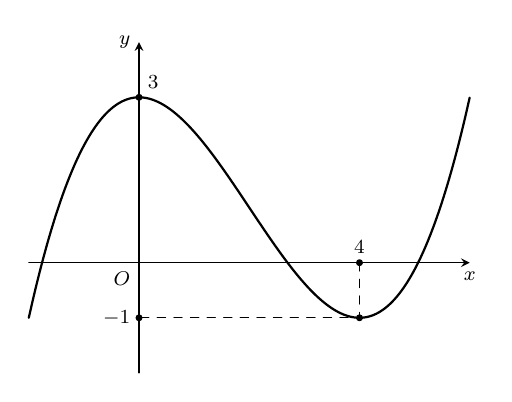
\begin{tikzpicture}[scale=0.7, font=\footnotesize, line join=round, line cap=round, >=stealth]
			\draw[->] (-2,0) -- (6,0) node[below] {$x$};
			\draw[->] (0,-2) -- (0,4) node[left] {$y$};
			\node[below left] at (0,0) {$O$};
			\draw[thick, smooth, samples=100, domain=-2:6] plot (\x, {0.125*(\x)^3 - 0.75*(\x)^2 + 3});
			\draw[dashed] (4,0) -- (4,-1) -- (0,-1);
			\draw[fill=black] (0,3) circle (1.5pt) node[above right] {$3$};
			\draw[fill=black] (4,-1) circle (1.5pt);
			\draw[fill=black] (4,0) circle (1.5pt) node[above] {$4$};
			\draw[fill=black] (0,-1) circle (1.5pt) node[left] {$-1$};
	\end{tikzpicture}}
	\loigiai{
		\begin{itemchoice}
			\itemch Dựa vào đồ thị, hàm số đạt cực đại tại điểm $x = 0$ và đạt cực tiểu tại điểm $x = 4$.
			\itemch Từ đồ thị, ta xác định các hệ số của hàm số $f(x)$
			\begin{itemize}
				\item Đồ thị cắt trục $Oy$ tại $(0; 3)$ nên $f(0) = 3 \Rightarrow d = 3$.
				\item Điểm cực đại tại $x = 0$ nên $f'(0) = 0 \Rightarrow c = 0$.
				\item Điểm cực tiểu tại $x = 4$ nên $f'(4) = 0 \Rightarrow 48a + 8b + c = 0 \Rightarrow 6a + b = 0$.
				\item Đồ thị đi qua điểm $(4; -1)$ nên 
				\[f(4) = -1 \Rightarrow 64a + 16b + 4c + d = -1 \Rightarrow 64a + 16b = -4 \Rightarrow 16a + 4b = -1.\]
			\end{itemize}
			Giải hệ phương trình $\heva{&6a + b = 0 \\ &16a + 4b = -1}$ ta được $a = \dfrac{1}{8}$, $b = -\dfrac{3}{4}$.\\
			Vậy $f(x) = \dfrac{1}{8}x^3 - \dfrac{3}{4}x^2 + 3$.\\
			Xét $g(x) = 26x - f(x) = -\dfrac{1}{8}x^3 + \dfrac{3}{4}x^2 + 26x - 3$ trên $[0; 4]$.\\
			$g'(x) = -\dfrac{3}{8}x^2 + \dfrac{3}{2}x + 26$. Trên đoạn $[0; 4]$, $g'(x) > 0$ nên hàm số $g(x)$ đồng biến.\\
			Suy ra $\max\limits_{[0; 4]} g(x) = g(4) = 26 \cdot 4 - f(4) = 104 -(-1) = 105$.
			\itemch Dựa vào đồ thị, hàm số đi xuống từ điểm cực đại $(0; 3)$ đến điểm cực tiểu $(4; -1)$ nên hàm số nghịch biến trên khoảng $(0; 4)$.
			\itemch Ta có $16a - 8b + 3c + d = 16 \cdot \dfrac{1}{8} - 8 \cdot \left(-\dfrac{3}{4}\right) + 3 \cdot 0 + 3 = 2 + 6 + 3 = 11$.
		\end{itemchoice}
	}
\end{ex}

\begin{ex}%[2D1H5-1]%[Dự án C - Đợt 3 - Sở Giáo Dục Sơn La]%[Hoàng Tuấn - Nguyễn Tiến]
	Cho hàm số $f(x)=x^3+3x^2-4$.
	\choiceTF
	{\True Hàm số đã cho có đạo hàm là $f'(x)=3x^2+6x$}
	{Hàm số đã cho đồng biến trên khoảng $(-1;+\infty)$}
	{\True Hàm số đã cho đạt cực đại tại $x=-2$}
	{\True Đồ thị của hàm số đã cho có dạng như hình vẽ sau}
	\begin{center}
		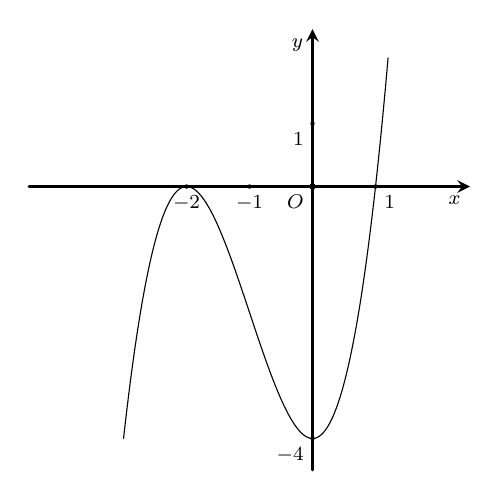
\begin{tikzpicture}[line join = round, line cap=round,>=stealth,font=\footnotesize,scale=0.8,samples=200]
			
			\def \xtrai{-4.5} \def\xphai{2.5}
			\draw[->,line width=1pt] (\xtrai,0)--(\xphai,0) coordinate (x) node[below left]{$x$};	
			\def \yduoi{-4.5} \def\ytren{2.5}
			
			\draw[->,line width=1pt] (0,\yduoi)--(0,\ytren)coordinate (y) node[below left]{$y$};			
			
			draw[opacity=0.1] (\xtrai,\yduoi) grid (\xphai,\ytren);
			\fill (0,0) coordinate (O) circle(1.5pt) node[below left]{$O$};
			\draw  plot[domain=-3:1.2] (\x,{(\x)^3+3*(\x)^2-4})
			;
			\foreach	\x	in	{-2,-1}
			\fill (\x,0) circle(1pt) node[below]{$\x$}
			;
			\foreach	\y	in	{-4,1}
			\fill (0,\y) circle(1pt) node[below left]{$\y$}
			;
			\foreach	\x	in	{1}
			\fill (\x,0) circle(1pt) node[below right]{$\x$};
		\end{tikzpicture}
	\end{center}
	\loigiai{
		\begin{itemchoice}
			\itemch  Đạo hàm của hàm số là $f'(x)=3x^2+6x$.
			\itemch  Xét $f'(x)=0\Leftrightarrow 3x^2+6x=0\Leftrightarrow \hoac{&x=0\\&x=-2.}$\\
			Bảng biến thiên
			\begin{center}
				
\begin{tikzpicture}
					\tkzTabInit[nocadre=false,lgt=1.2,espcl=2.5,deltacl=0.6]
					{$x$/0.6,$f'(x)$/0.6,$f(x)$/2}{$-\infty$,$-2$,$0$,$+\infty$}
					\tkzTabLine{,+,0,-,0,+}
					\tkzTabVar{-/$-\infty$,+/$0$,-/$-4$,+/$+\infty$}
				\end{tikzpicture}
			\end{center}
			Từ bảng biến thiên ta thấy hàm số đồng biến trên khoảng $(0;+\infty)$.
			\itemch  Từ bảng biến thiên ta thấy hàm số đạt cực đại tại $x=-2$.
			\itemch Ta thấy tại $x=-2$ thì $y=0$; tại $x=0$ thì $y=-4$.\\
			Do đó đồ thị hàm số đã cho có dạng như hình vẽ sau
			\begin{center}
				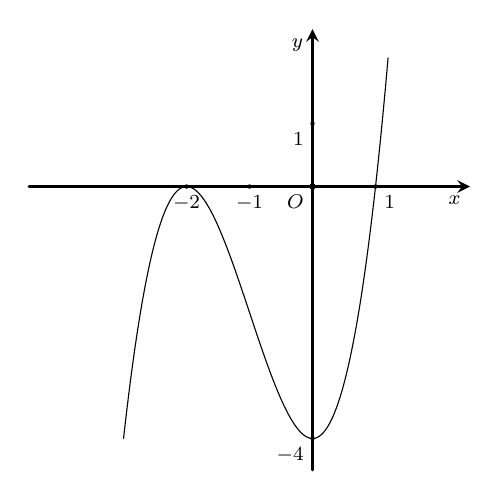
\begin{tikzpicture}[line join = round, line cap=round,>=stealth,font=\footnotesize,scale=0.8,samples=200]
					
					\def \xtrai{-4.5} \def\xphai{2.5}
					\draw[->,line width=1pt] (\xtrai,0)--(\xphai,0) coordinate (x) node[below left]{$x$};	
					\def \yduoi{-4.5} \def\ytren{2.5}
					
					\draw[->,line width=1pt] (0,\yduoi)--(0,\ytren)coordinate (y) node[below left]{$y$};			
					
					draw[opacity=0.1] (\xtrai,\yduoi) grid (\xphai,\ytren);
					\fill (0,0) coordinate (O) circle(1.5pt) node[below left]{$O$};
					\draw  plot[domain=-3:1.2] (\x,{(\x)^3+3*(\x)^2-4})
					;
					\foreach	\x	in	{-2,-1}
					\fill (\x,0) circle(1pt) node[below]{$\x$}
					;
					\foreach	\y	in	{-4,1}
					\fill (0,\y) circle(1pt) node[below left]{$\y$}
					;
					\foreach	\x	in	{1}
					\fill (\x,0) circle(1pt) node[below right]{$\x$};
				\end{tikzpicture}
			\end{center}
		\end{itemchoice}
	}
\end{ex}

\begin{ex}%[2D1H5-8]%[Dự án C đề thi thử TN Môn Toán NH25-26 - Dot 4 - Trung Kiên]%[THPT Phan Bội Châu-Khánh Hòa]%[GVPB - Phạm Văn Long]		
	Cho hàm số $y=f(x)=\dfrac{3x+5}{2x+2}$ có đồ thị là $(C)$.
	\choiceTF
	{Giá trị lớn nhất của hàm số $f(x)$ trên $[1;3]$ bằng $\dfrac{7}{4}$}
	{Tâm đối xứng của $(C)$ là điểm $I\left(1;\dfrac{3}{2}\right)$}
	{\True Hàm số $f(x)$ không có cực trị}
	{Một công ty sản xuất $x$ sản phẩm $(x \ge 1)$ thì chi phí sản xuất trung bình một sản phẩm được tính theo công thức $\overline{C}(x)=250f(x)$ (nghìn đồng). Khi đó số lượng sản phẩm sản xuất càng lớn thì chi phí sản xuất trung bình một sản phẩm sẽ giảm dần và luôn thấp hơn $375$ nghìn đồng}
	\loigiai{
		\begin{itemchoice}
			\itemch Tập xác định $\mathscr{D}=\mathbb{R}\setminus\{-1\}$. Suy ra hàm số $y=f(x)$ liên tục trên đoạn $[1;3]$.\\
			Ta có $f'(x) = -\dfrac{4}{(2x+2)^2} < 0, \forall x \neq -1$ và $f(1)=2$, $f(3)=\dfrac{7}{4}$.\\
			Vậy $\max\limits_{[1;3]} f(x) = f(1)=2$.
			\itemch Do $\lim\limits_{x\to -1^+} \dfrac{3x+5}{2x+2} = +\infty$ nên đường thẳng $x=-1$ là đường tiệm cận đứng của đồ thị $(C)$.\\
			Do $\lim\limits_{x\to +\infty} \dfrac{3x+5}{2x+2} = \dfrac{3}{2}$ nên đường thẳng $y=\dfrac{3}{2}$ là đường tiệm cận ngang của đồ thị $(C)$.\\
			Tâm đối xứng của $(C)$ là giao điểm của đường tiệm cận đứng và đường tiệm cận ngang nên tâm đối xứng của $(C)$ là điểm $\left(-1;\dfrac{3}{2}\right)$.
			\itemch Hàm số $y=f(x)=\dfrac{3x+5}{2x+2}$ có tập xác định $\mathscr{D}=\mathbb{R}\setminus\{-1\}$ và
			$$f'(x)=-\dfrac{4}{(2x+2)^2} < 0, \forall x \neq -1.$$
			Do đó hàm số $f(x)$ không có cực trị.
			\itemch Xét $h(x)=\overline{C}(x) = 250 \cdot \dfrac{3x+5}{2x+2}$.\\
			Ta có $h'(x)= 250 \cdot \dfrac{-4}{(2x+2)^2} = \dfrac{-1\,000}{(2x+2)^2} < 0, \forall x \ge 1$.\\
			Bảng biến thiên
			\begin{center}
				
\begin{tikzpicture}
					\tkzTabInit[nocadre=false,lgt=1.2,espcl=5,deltacl=0.4]
					{$x$/1,$h'(x)$/1,$h(x)$/1.5}
					{$1$,$+\infty$}
					\tkzTabLine{,-,}
					\tkzTabVar{+/$500$,-/$375$}
				\end{tikzpicture}
			\end{center}
			Số lượng sản phẩm sản xuất càng lớn thì chi phí sản xuất trung bình một sản phẩm sẽ giảm dần và luôn cao hơn 375 nghìn đồng.
		\end{itemchoice}
	}
\end{ex}

\begin{ex}%[2D1V3-1]%[Dự án C đợt 3 NH25-26]%[GVBS-GVPB Thanh Phát]
	Cho hàm số $f(x) = 92 - 20\ln(x+1)$.
	\choiceTF
	{\True Tập xác định của hàm số đã cho là $\mathscr{D} = (-1; +\infty)$}
	{Bất phương trình $f(x) \geq 36$ có đúng $15$ nghiệm nguyên}
	{Hàm số đã cho đồng biến trên khoảng $(-1; +\infty)$}
	{Giá trị lớn nhất của hàm số $g(x) = f(x) + 5x$ trên đoạn $[1; 4]$ bằng $107 - 40\ln 2$}
	\loigiai{
		\begin{itemchoice}
			\itemch Hàm số xác định khi và chỉ khi $x+1 > 0 \Leftrightarrow x > -1$.\\
			Vậy tập xác định của hàm số là $\mathscr{D} = (-1; +\infty)$.
			\itemch Ta có 
			\allowdisplaybreaks
			\begin{eqnarray*}
				& &f(x) \geq 36\\
				&\Leftrightarrow& 92 - 20\ln(x+1) \geq 36\\
				&\Leftrightarrow& \ln(x+1) \leq 2{,}8\\
				&\Leftrightarrow&x+1 \leq \mathrm{e}^{2{,}8}\\
				&\Leftrightarrow&x\leq \mathrm{e}^{2{,}8} - 1.
			\end{eqnarray*}
			So với điều kiện xác định $x > -1$, ta được $-1 < x \leq \mathrm{e}^{2{,}8} - 1$.\\
			Vì $x \in \mathbb{Z}$ nên $x \in \{0; 1; 2; \ldots; 15\}$.\\
			Vậy bất phương trình có $16$ nghiệm nguyên.
			\itemch Ta có $f'(x) = \dfrac{-20}{x+1} < 0$ với mọi $x \in (-1; +\infty)$.\\
			Do đó hàm số nghịch biến trên khoảng $(-1; +\infty)$.
			\itemch Ta có $g(x) = f(x) + 5x = 92 - 20\ln(x+1) + 5x$ xác định trên đoạn $[1; 4]$.\\
			Ta có $g'(x) = \dfrac{-20}{x+1} + 5 = \dfrac{5x - 15}{x+1}$.\\
			Cho $g'(x) = 0 \Leftrightarrow 5x - 15 = 0 \Leftrightarrow x = 3 \in [1; 4]$.\\
			Ta có
			\begin{itemize}
				\item $g(1) = 97 - 20\ln 2 \approx 83{,}14$.
				\item $g(3) = 107 - 40\ln 2 \approx 79{,}27$.
				\item $g(4) = 112 - 20\ln 5 \approx 79{,}81$.
			\end{itemize}
			Vậy $\max\limits_{[1; 4]} g(x) = g(1) = 97 - 20\ln 2$.
		\end{itemchoice}
	}
\end{ex}

\begin{ex}%[2D1V3-1]%[Dự án đề TT-THPT-TranNhanTong-HaNoi-N25-26-Dot 3- Nguyễn Văn Nghĩa]%[SGD Hà Nội] %[GVPB - Phan Quốc Trí]
	Cho hàm số $f(x) = \sin 2x - 2x$.
	\choiceTF
	{Đạo hàm của hàm số đã cho là $f'(x) = \cos 2x - 2$}
	{\True Hàm số nghịch biến trên tập xác định}
	{\True Nghiệm dương lớn nhất của phương trình $f'(x) + 1 = 0$ trên đoạn $[-\pi; \pi]$ là $\dfrac{5\pi}{6}$}
	{Giá trị nhỏ nhất của $f(x)$ trên đoạn $\left[0; \dfrac{\pi}{6}\right]$ là $-\dfrac{\pi}{3} + \sqrt{3}$}
	\loigiai{
		
		\begin{itemchoice}
			\itemch 
			Ta có $f'(x) = 2\cos 2x - 2$.
			\itemch 
			Vì $\cos 2x \leq 1$ suy ra $f'(x)=2\cos 2x - 2 \leq 0, \forall x \in \mathbb{R}$.\\
			Và $f'(x)=0$ khi $x=k\pi$ với $(k\in\mathbb{Z})$.\\
			Vậy hàm số nghịch biến trên $\mathbb{R}$.
			\itemch 
			$f'(x) + 1 = 0\Leftrightarrow2\cos 2x - 1=  0\Leftrightarrow\cos 2x=  \dfrac{1}{2}\Leftrightarrow x=\pm \dfrac{\pi}{6} + k\pi$.\\
			Các nghiệm $x\in\left[-\pi; \pi\right]$ là $-\dfrac{5\pi}{6}$, $-\dfrac{\pi}{6}, \dfrac{\pi}{6}$ và $\dfrac{5\pi}{6}$. Do đó nghiệm dương lớn nhất là $\dfrac{5\pi}{6}$.
			\itemch 
			Vì hàm số nghịch biến nghịch biến trên $\mathbb{R}$ nên hàm số nghịch biến trên $\left[0; \dfrac{\pi}{6}\right]$.\\
			Suy ra $\min\limits_{x\in \left[0; \tfrac{\pi}{6}\right]} f(x)=f\left(\dfrac{\pi}{6}\right)= \sin\left(\dfrac{\pi}{3}\right) - 2\left(\dfrac{\pi}{6}\right) = \dfrac{\sqrt{3}}{2} - \dfrac{\pi}{3}$.
		\end{itemchoice}
	}
\end{ex}

\begin{ex}%[2D1V3-6]%[Dự án C đề thi thử TN Môn Toán NH25-26 - Dot 4 - Võ Thị Thùy Trang]%[Liên trường THPT cụm 09 - Đợt 2 - Hà Nội]%[GVPB - Thanh Phát]
	Trong buổi tổng duyệt văn nghệ tại sân trường, một drone được sử dụng để ghi hình toàn cảnh. Trong $15$ giây đầu kể từ khi cất cánh, do hệ thống tự động điều chỉnh lực đẩy để tiết kiệm pin, độ cao của drone (tính bằng mét) tại thời điểm $t$ giây, được mô tả gần đúng bởi $h(t)=-0{,}05t^3+0{,}6t^2+3t$ ($0 \le t \le 15$). Cùng thời điểm đó, một thang nâng sân khấu bắt đầu nâng thẳng đứng từ mặt sân với vận tốc không đổi $1$\,m/s.
	\choiceTF
	{\True Vận tốc của drone tại thời điểm $t$ là $v(t)=-0{,}15t^2+1{,}2t+3$}
	{Drone luôn bay lên trong $12$ giây đầu}
	{\True Trong khoảng $0<t\le 15$, drone và thang nâng ở cùng độ cao đúng $1$ lần}
	{Độ cao lớn nhất mà drone đạt được trong $15$ giây đầu không vượt quá $39$\, m}
	\loigiai{
		\begin{itemchoice}
			\itemch Vận tốc của drone là $v(t)=h'(t)=-0{,}15t^2+1{,}2t+3$.
			\itemch Drone bay lên khi và chỉ khi\\
			\[v(t)>0 \Leftrightarrow -0{,}15t^2+1{,}2t+3>0 \Leftrightarrow 0<t<10.\]
			Suy ra drone luôn bay lên trong $10$ giây đầu.
			\itemch Thang nâng từ mặt sân với vận tốc không đổi $1$\,m/s suy ra độ cao của thang nâng tại thời điểm $t$ giây là $g(t)=t$\,(m).\\
			Drone và thang nâng cùng độ cao khi và chỉ khi
			\allowdisplaybreaks
			\begin{eqnarray*}
				h(t)=g(t) &\Leftrightarrow & -0{,}05t^3+0{,}6t^2+3t=t\\
				&\Leftrightarrow & -0{,}05t^3+0{,}6t^2+2t=0\\
				&\Leftrightarrow & \hoac{&t=0 &&\text{ (loại)}\\&t=6+\sqrt{76} &&\text{ (nhận)}\\&t=6-\sqrt{76} &&\text{ (loại)}.}\\
			\end{eqnarray*}
			Vậy drone và thang nâng cùng độ cao đúng $1$ lần.
			\itemch Xét hàm số $h(t)=-0{,}05t^3+0{,}6t^2+3t$ liên tục trên đoạn $[0;15]$.\\
			$h'(t)=0 \Leftrightarrow -0{,}15t^2+1{,}2t+3=0 \Leftrightarrow \hoac{&t=10 \in (0;15)\\&t=-2 \notin (0;15).}$\\
			$h(0)=0$, $h(10)=40$, $h(15)=11{,}25$.\\
			Độ cao lớn nhất của drone trong $15$ giây đầu là $40$\,m $> 39$\,m.
		\end{itemchoice}
	}
\end{ex}

\begin{ex}%[Đề thi thử môn Toán TRƯỜNG THPT LÊ THÁNH TÔNG-TP. HCM năm học 2025-2026]%[Tên GV soạn: Quốc Dũng - GV phản biện: Phan Anh]%[2D1V4-1]
	Cho hàm số $y=f\left(x\right)=\dfrac{-x^2+10x-12}{x}$ có đồ thị là $(C)$ và hình vẽ sau:
	\begin{center}
	\begin{tikzpicture}[line join=round, line cap=round,>=stealth,thick,scale=0.9]
%	\def\xmax{13} \def\xmin{-2} \def\ymax{7} \def\ymin{-3}
%	\draw[step=1cm, gray!30, thin] (-3,-3) grid (15,15);
%	\draw[->] (\xmin,0) -- (\xmax,0)  node[left] {\footnotesize  $x$};
%	\draw[->] (0,\ymin) -- (0,\ymax) node[left] {\footnotesize  $y$};
	\coordinate[label=above left:$A$] (A) at (-5,3.5);
	\coordinate[label=above left:$B$] (B) at (2,2);
	\coordinate[label=below :$C$] (C) at (0,-2);	
		\begin{scope}
			\draw[samples=200,domain=1.001:12,smooth,variable=\x] plot (\x,{(-1*(\x)^2+10*(\x)-12)/((\x))});
			\draw[dashed,thin] (1,-3)--(12,-3);
		\end{scope}
%		\draw[samples=200,domain=1.001:12,smooth,variable=\x] plot (\x,{(2*(\x)-2)});
		\fill[ olive!20] (1,-3)--plot[domain=1:12] (\x,{(-1*(\x)^2+10*(\x)-12)/((\x))})--(12,-3);
		\fill[ cyan!20] (A)--(B)-- (C)--cycle;
		\draw[thin] (B)--(A)--(C)--cycle;
		\draw[magenta] (-0.5,1) node [below ] {\text{Ao nuôi tôm}};
		\draw[magenta] (6,-1) node [below left] {\text{Phần đất}};
		\draw(5,3) node [right] {$(C)$};
		\foreach \diem in {A,B,C}	\fill (\diem)circle(1.5pt);
	\end{tikzpicture}
\end{center}
	\choiceTF
	{ Hàm số $y=f\left( x \right)$ đồng biến trên khoảng $\left( 0;\dfrac{7}{2} \right)$}
	{\True Đồ thị hàm số $y=f\left( x \right)$ có đường tiệm cận xiên là $y=-x+10$}
	{Khoảng cách giữa hai điểm cực trị của đồ thị hàm số là $4\sqrt{15}$}
	{\True Trong mặt phẳng toạ độ $Oxy$ (đơn vị mỗi trục là $1$ m) mô hình hoá một phần đồ thị hàm số $y=f(x)=\dfrac{-x^2+10x-12}{x}$$\left( x>0 \right)$ là bờ của phần đất nhô ra. Người ta muốn xây một ao nuôi tôm dạng hình tam giác $ABC$ với $A(-6;6)$, đường thẳng $BC$ là tiếp tuyến với $(C)$ nhận $B$ làm tiếp điểm và $BC=10$ m. Diện tích ao nuôi tôm lớn nhất là $20\sqrt{5}\text{m}^2$}
	\loigiai{
		\begin{itemchoice}
			\itemch $y=f\left( x \right)=\dfrac{-x^2+10x-12}{x}$\\
		Ta có	$f'\left( x \right)=\dfrac{-x^2+12}{x^2}$.
			Cho $f'\left( x \right)=0\Leftrightarrow \dfrac{-x^2+12}{x^2}=0 \Leftrightarrow $
		$	\hoac{ & x=-2\sqrt{3} \\ 
				& x=2\sqrt{3}. \\ 
			}$ \\
			$\underset{x\to-\infty}{\mathop{\lim }}f\left(x\right)=+\infty ;\underset{x\to +\infty }{\mathop{\lim }}f\left( x \right)=-\infty$;
			$\underset{x\to 0^-}{\mathop{\lim }}f\left( x \right)=+\infty ;\underset{x\to 0^+}{\mathop{\lim }}f\left( x \right)=-\infty $.\\
			Bảng biến thiên của hàm số $y=f\left( x \right)$
			\begin{center}
			
\begin{tikzpicture}
				\tkzTabInit[espcl=3,lgt=1.5]
				{$x$/0.7,$f'\left( x \right)$/0.7,$f\left( x \right)$/2.1}
				{$-\infty$,$-2\sqrt{3}$ ,$0$,$2\sqrt{3}$,$+\infty$}
				\tkzTabLine{,-,0,+,d,+,0,-,}
				\tkzTabVar{+/$+\infty$,-/$10+4\sqrt{3}$,+D-/$+\infty$/$-\infty$,+/$10-4\sqrt{3}$,-/$-\infty$,}
			\end{tikzpicture}
		\end{center}
			Hàm số đồng biến trên các khoảng $\left( -2\sqrt{3};0 \right)$ và $\left( 0;2\sqrt{3} \right)$.
			\itemch $y=f\left( x \right)=\dfrac{-x^2+10x-12}{x}\Rightarrow f\left( x \right)=-x+10-\dfrac{12}{x}$.\\
		Ta có	 $\heva{
				&\underset{x\to +\infty }{\mathop{\lim}}\left( f\left( x \right)-(-x+10)\right)=\underset{x\to +\infty}{\mathop{\lim}}\left( -\dfrac{12}{x} \right)=0 \\ 
				& \underset{x\to -\infty}{\mathop{\lim}}\left(f\left( x \right)-(-x+10) \right)=\underset{x\to -\infty }{\mathop{\lim }}\left( -\dfrac{12}{x}\right)=0\\ 
			} $
		
			Đồ thị hàm số có đường tiệm cận xiên là $y=-x+10$.
			\itemch Đồ thị hàm số có hai điểm cực trị là $M\left( -2\sqrt{3};10+4\sqrt{3} \right);N\left( 2\sqrt{3};10-4\sqrt{3} \right)$. Suy ra
			$\overrightarrow{MN}=\left( 4\sqrt{3};-8\sqrt{3} \right)$$\Rightarrow MN=4\sqrt{15}$. 
			\itemch 
				\begin{center}
				\begin{tikzpicture}[line join=round, line cap=round,>=stealth,thick,scale=0.9]
					%	\def\xmax{13} \def\xmin{-2} \def\ymax{7} \def\ymin{-3}
					%	\draw[step=1cm, gray!30, thin] (-3,-3) grid (15,15);
					%	\draw[->] (\xmin,0) -- (\xmax,0)  node[left] {\footnotesize  $x$};
					%	\draw[->] (0,\ymin) -- (0,\ymax) node[left] {\footnotesize  $y$};
					\coordinate[label=above left:$A$] (A) at (-5,3.5);
				\coordinate[label=above :$B$] (B) at (2,2);
				\coordinate[label=below :$C$] (C) at (0,-2);
					\coordinate[label=below :$H$] (H) at ($(B)!(A)!(C)$);	
					\begin{scope}
						\draw[samples=200,domain=1.001:12,smooth,variable=\x] plot (\x,{(-1*(\x)^2+10*(\x)-12)/((\x))});
						\draw[dashed,thin] (1,-3)--(12,-3);
					\end{scope}
					\fill[ olive!20] (1,-3)--plot[domain=1:12] (\x,{(-1*(\x)^2+10*(\x)-12)/((\x))})--(12,-3);
					\fill[ cyan!20] (A)--(B)-- (C)--cycle;
					\draw[thin] (B)--(A)--(C)--cycle (A)--(H);
					\draw[magenta] (0.5,1) node [below left] {\text{Ao nuôi tôm}};
					\draw[magenta] (6,-1) node [below left] {\text{Phần đất}};
					\draw(5,3) node [right] {$(C)$};
					\foreach \diem in {A,B,C,H}	\fill (\diem)circle(1.5pt);
				\end{tikzpicture}
			\end{center}
			Gọi $H$ là hình chiếu của $A$ trên $BC$ khi đó
			${{S}_{\Delta ABC}}=\dfrac{1}{2}AH \cdot BC=5 \cdot AH$.
			Suy ra diện tích tam giác $ABC$ lớn nhất khi $AH$ lớn nhất.\\
			Ta có $AH\le AB$$\Rightarrow AH$ lớn nhất khi $H\equiv B\Rightarrow BC\bot AB$.\\
			Do đó tiếp tuyến $BC$ có véctơ pháp tuyến là $\overrightarrow{AB}$.\\
			Gọi $B\left( b;f(b)\right)(b>0)$;
			$\overrightarrow{AB}=\left( b+6;-b+4-\dfrac{12}{b} \right)$, $f'\left( b \right)=-1+\dfrac{12}{b^2}$.\\
			Đường thẳng $BC$ có véc tơ chỉ phương $\overrightarrow{u}\left( 1;-1+\dfrac{12}{b^2} \right)$. Mặt khác
		\begin{eqnarray*}
	 AB\bot BC&\Rightarrow& \overrightarrow{AB}.\overrightarrow{u}=0\\
			&\Rightarrow& b+6+\left( -b+4-\dfrac{12}{b} \right)\left( -1+\dfrac{12}{b^2} \right)
			=0\\
			&\Rightarrow& 2b^4+2b^3+48b-144
			=0\\
			&\Rightarrow& b
			=2.
		\end{eqnarray*}
				 Suy ra $\overrightarrow{AB}=\left( 8;-4 \right)\Rightarrow AB=4\sqrt{5}$. Vậy	${{S}_{\Delta ABC}}=5\cdot AB=20\sqrt{5}$.
	\end{itemchoice}
	}
\end{ex}

\begin{ex}%[2D1V4-1]%[Dự án C đề thi thử TN Môn Toán NH25-26 - Dot 4 - BCTuan]%[THPT Nguyễn Trãi-Hà Nội]%[GVPB-Khắc Thiên]
	Cho hàm số $y=\dfrac{x^2-3x+6}{x-1}$.
	\choiceTF
	{\True Tọa độ điểm cực tiểu của đồ thị hàm số là $(a;b)$. Khi đó, ta có $a^2+b=12$}
	{\True Tiệm cận xiên của đồ thị hàm số là $y=x-2$}
	{Gọi $I$ là giao điểm hai đường tiệm cận của đồ thị hàm số. Tiếp tuyến của đồ thị hàm số tại điểm có hoành độ $x=2$ cắt hai đường tiệm cận tại $A$, $B$. Diện tích tam giác $IAB$ bằng $12$}
	{\True Có tất cả $9$ giá trị nguyên của tham số $m$ để phương trình $\dfrac{x^2-3x+6}{x-1}=m$ có hai nghiệm phân biệt $x_1$, $x_2$ thỏa mãn $x_1<2<x_2<15$}
	\loigiai{
		\begin{itemchoice}
			\itemch Tập xác định $\mathscr{D}=\mathbb{R}\setminus\{1\}$.\\
			Ta có $y = \dfrac{x^2-3x+6}{x-1} = x - 2 + \dfrac{4}{x-1}$.\\
			Khi đó $y' = 1 - \dfrac{4}{(x-1)^2} = \dfrac{x^2-2x-3}{(x-1)^2}$.\\ 		
			Xét $y' = 0 \Leftrightarrow \hoac{&x = -1\\&x = 3.}$\\
			Bảng biến thiên
			\begin{center}
				
\begin{tikzpicture}
					\tikzset{double style/.append style={double distance=1.5pt}}
					\tkzTabInit[nocadre=false,lgt=1.2,espcl=2.5,deltacl=0.6]
					{$x$ /0.8,$y'$ /0.8,$y$ /2.2}
					{$-\infty$,$-1$,$1$,$3$,$+\infty$}
					\tkzTabLine{,+,0,-,d,-,0,+,}
					\tkzTabVar{-/$-\infty$,+/$-5$,-D+/$-\infty$/$+\infty$,-/$3$,+/$+\infty$}
				\end{tikzpicture}
			\end{center}
			Đồ thị hàm số đạt cực tiểu tại điểm có hoành độ $x=3$.\\
			Suy ra giá trị cực tiểu $y(3)=3$.\\
			Tọa độ điểm cực tiểu của đồ thị là $(3;3)$.\\
			Suy ra $a=3$, $b=3$.\\
			Khi đó $a^2+b = 3^2+3 = 12$.			
			\itemch Ta có $\lim\limits_{x \to \pm\infty} [y - (x-2)] = \lim\limits_{x \to \pm\infty} \dfrac{4}{x-1} = 0$.\\
			Do đó đường thẳng $y=x-2$ là tiệm cận xiên của đồ thị hàm số.			
			\itemch Tiệm cận đứng $x=1$, tiệm cận xiên $y=x-2$.\\ 
			Giao điểm $I(1;-1)$.\\
			Tại $x=2 \Rightarrow y(2)=4$ và $y'(2) = -3$.\\
			Phương trình tiếp tuyến $\Delta$ tại $x=2$ là $y = -3(x-2)+4 \Leftrightarrow y = -3x+10$.\\
			Giao điểm của $\Delta$ với tiệm cận đứng $x=1$ là $A(1;7)$.\\
			Giao điểm của $\Delta$ với tiệm cận xiên $y=x-2$ là nghiệm của hệ \[\heva{&y = -3x+10\\&y = x-2} \Leftrightarrow \heva{&x = 3\\&y = 1} \Rightarrow B(3;1).\]
			Độ dài $IA = \sqrt{(1-1)^2 + (7 - (-1))^2} = 8$.\\
			Đường thẳng $IA$ có phương trình $x=1$.\\
			Khoảng cách từ $B(3;1)$ đến đường thẳng $IA$ là $\mathrm{d} = |3-1| = 2$.\\
			Diện tích tam giác $IAB$ là $S = \dfrac{1}{2} \cdot IA \cdot \mathrm{d} = \dfrac{1}{2} \cdot 8 \cdot 2 = 8$.			
			\itemch Phương trình $\dfrac{x^2-3x+6}{x-1}=m \Leftrightarrow x^2 - (m+3)x + m+6 = 0 \quad (1)$ (với $x \neq 1$).\\
			Đặt $g(x) = x^2 - (m+3)x + m+6$.\\ 
			Phương trình có hai nghiệm thỏa $1\ne x_1<2<x_2<15$ khi và chỉ khi
			\allowdisplaybreaks
			\begin{eqnarray*}
				&&\heva{&g(1)\ne 0\\&g(2) < 0\\&g(15) > 0}\\
				&\Leftrightarrow& \heva{&1 - (m+3) + m+6 = 4 \neq 0 \text{ (luôn đúng)}\\&4 - 2(m+3) + m+6 < 0\\&225 - 15(m+3) + m+6 > 0}\\
				&\Leftrightarrow& \heva{&4 - m < 0\\&186 - 14m > 0}\\
				&\Leftrightarrow& \heva{&m > 4\\&m < \dfrac{93}{7}}\\
				&\Leftrightarrow& 4 < m < \dfrac{93}{7} \approx 13{,}28.
			\end{eqnarray*}
			Vì $m \in \mathbb{Z}$ nên $m \in \{5;\, 6;\, 7;\, 8;\, 9;\, 10;\, 11;\, 12;\, 13\}$.\\
			Vậy có tất cả $9$ giá trị nguyên của $m$ thỏa mãn.
		\end{itemchoice}
	}
\end{ex}

\begin{ex}%[2D1V4-3]%%[Dự án đề TT Toán NH25-26-Dot3-Đắc Vũ]%[Cụm 13-Hải Phòng]%[GVPB-Viet Hoang Pham]
	Cho hàm số $y = \dfrac{x^2 - x + 1}{x + 1}$ có đồ thị $(C)$.
	\choiceTF
	{\True Hàm số có cực đại, cực tiểu}
	{Giao điểm hai đường tiệm cận của đồ thị $(C)$ có tọa độ là $(-1; 3)$}
	{\True Đường tiệm cận xiên của đồ thị $(C)$ cắt trục hoành, trục tung tại các điểm $A, B$ và diện tích tam giác $OAB$ bằng $2$ ($O$ là gốc tọa độ)}
	{Gọi $MNPQ$ là hình vuông có tâm $I$ là giao điểm hai đường tiệm cận và hai đỉnh $M, P$ lần lượt nằm trên hai nhánh khác nhau của đồ thị $(C)$. Hình vuông $MNPQ$ có diện tích nhỏ nhất bằng $12\left(\sqrt{2}-1\right)$}
	\loigiai{
		\begin{itemchoice}
			\itemch 
			
			Hàm số xác định với mọi $x \ne -1$.\\
			Ta có $y = x - 2 + \dfrac{3}{x+1}$ nên $y' = 1 - \dfrac{3}{(x+1)^2} = \dfrac{x^2+2x-2}{(x+1)^2}$.\\
			Suy ra $y' = 0 \Leftrightarrow x^2+2x-2 = 0 \Leftrightarrow x = -1 \pm \sqrt{3}$.\\
			Vậy hàm số có cực đại, cực tiểu.
			
			\itemch 
			
			Đồ thị $(C) \colon y = \dfrac{x^2-x+1}{x+1}$ có đường tiệm cận đứng $x = -1$ và đường tiệm cận xiên $y = x - 2$.\\
			Vậy giao điểm hai đường tiệm cận là điểm $(-1; -3)$.
			
			\itemch 
			
			Đường tiệm cận xiên $y = x - 2$ cắt trục hoành tại điểm $A(2; 0)$ và cắt trục tung tại điểm $B(0; -2)$.\\
			Diện tích tam giác $OAB$ bằng $\dfrac{1}{2} \cdot OA \cdot OB = \dfrac{1}{2} \cdot 2 \cdot 2 = 2$.
			
			\itemch 
			
			Giả sử đỉnh $M\left(-1+a; -3+a+\dfrac{3}{a}\right)$ ($a>0$) nằm ở nhánh bên phải tiệm cận đứng của đồ thị $(C)$.\\
			Ta có $MNPQ$ là hình vuông có tâm $I$ nên $S_{MNPQ} = 2IM^2$.\\
			Do $\overrightarrow{IM} = \left(a; a+\dfrac{3}{a}\right)$ nên $IM^2 = a^2 + \left(a+\dfrac{3}{a}\right)^2 = 2a^2 + \dfrac{9}{a^2} + 6 \ge 2\sqrt{2a^2 \cdot \dfrac{9}{a^2}} + 6$.\\
			Suy ra $S_{MNPQ} \ge 2\left(6\sqrt{2} + 6\right) \Rightarrow S_{MNPQ} \ge 12\left(\sqrt{2}+1\right)$.\\
			Vậy hình vuông $MNPQ$ có diện tích nhỏ nhất bằng $12\left(\sqrt{2}+1\right)$.
		\end{itemchoice}
	}
\end{ex}

\begin{ex}%[Đề thi thử môn Toán THPT Hàm Rồng năm học 2025-2026]%[Nguyễn Khánh Trọng - GVPB2 Đỗ Minh Vũ]%[2D1V5-4]
	Cho hàm số $y=\dfrac{x+1}{x-1}$ có đồ thị $(C)$.
	\choiceTF
	{\True Hàm số nghịch biến trên khoảng $(1;+\infty)$}
	{\True Biết cả hai đường thẳng $d_1\colon y=a_1x+b_1$; $d_2\colon y=a_2x+b_2$ đi qua điểm $I(1;1)$, cắt đồ thị $(C)$ tại $4$ điểm tạo thành một hình chữ nhật có $a_1+a_2=\dfrac{5}{2}$. Khi đó giá trị biểu thức $b_1\cdot b_2=-\dfrac{1}{2}$}
	{\True Giá trị lớn nhất của hàm số trên $[2;5]$ là $3$}
	{Đường tiệm cận đứng của đồ thị hàm số có phương trình $y=1$}
	\loigiai{
		\begin{itemchoice}
			\itemch Tập xác định $\mathscr{D}=\mathbb{R}\setminus\{1\}$.\\
			Ta có $y'=\dfrac{-2}{\left(x-1\right)^2}$, suy ra $y'<0$, $\forall x\ne 1$.\\
			Suy ra hàm số nghịch biến trên các khoảng $(-\infty;1)$ và $(1;+\infty)$.
			\itemch 
			\begin{center}
				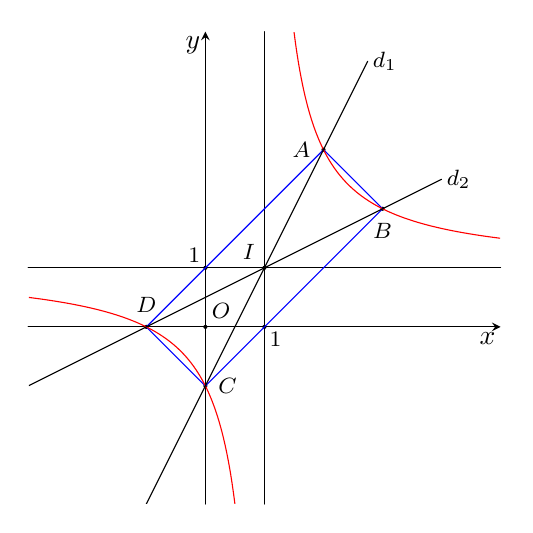
\begin{tikzpicture}[line join=round,line cap=round,>=stealth,scale=0.75,font=\footnotesize]
					\tikzset{every node/.style={outer sep=-0.5mm}}
					\def \xmin{-3} \def \xmax{5}
					\def \ymin{-3} \def \ymax{5}
					\def \fx{(\x+1)/(\x-1)}
					\def \gx{2*(\x)-1}
					\def \hx{0.5*(\x)+0.5}
					\draw[->] (\xmin,0)--(\xmax,0) node[below left] {\normalsize$x$};
					\draw[->] (0,\ymin)--(0,\ymax) node[below left] {\normalsize$y$};
					\draw (\xmin,1)--(\xmax,1) (1,\ymin)--(1,\ymax);
					\foreach \x in {1} \fill (\x,0) circle (1pt) node[below right] {$\x$};
					\foreach \y in {1} \fill (0,\y) circle (1pt) node[above left] {$\y$};
					\foreach \x/\y/\n in {2/3/A,3/2/B,0/-1/C,-1/0/D,0/0/O,1/1/I} \coordinate (\n) at (\x,\y);
					\foreach \t/\g in {A/180,B/-90,C/0,D/90,O/45,I/135}{
						\fill (\t) circle (1pt) node[shift={(\g:8pt)}]{$ \t $};
					}
					\draw[blue] (A)--(B)--(C)--(D)--(A);
					\begin{scope}
						\clip (\xmin+0.01,\ymin+0.01) rectangle (\xmax-0.01,\ymax-0.01);
						\draw[red,samples=150,domain=1+0.01:\xmax-0.01,smooth,variable=\x] plot (\x,{\fx});
						\draw[red,samples=150,domain=\xmin+0.01:1-0.01,smooth,variable=\x] plot (\x,{\fx});
						\draw[samples=150,domain=\xmin+0.01:2.75,smooth,variable=\x] plot (\x,{\gx}) node[right]{$d_1$};
						\draw[samples=150,domain=\xmin+0.01:4,smooth,variable=\x] plot (\x,{\hx})node[right]{$d_2$};
					\end{scope}
				\end{tikzpicture}
			\end{center}
			Gọi $\alpha$, $\beta$ lần lượt là góc tạo bởi $d_1$, $d_2$ với trục $Ox\Rightarrow{a_1}=\tan\alpha$, $a_2=\tan\beta $.\\
			Để hai đường thẳng $d_1$, $d_2$ cắt đồ thị $(C)$ tại $4$ điểm tạo thành một hình chữ nhật $ABCD$ thì $ABCD$ phải nhận đường thẳng $y=x$ làm trục đối xứng và nhận $I(1;1)$ làm tâm đối xứng.\\
			Khi đó $\alpha+\beta=90^\circ\Rightarrow\tan\alpha=\cot\beta\Rightarrow{a_1}=\dfrac{1}{a_2}\Rightarrow a_1\cdot a_2=1$.\\
			Ta có $\heva{&a_1+a_2=\dfrac{5}{2}\\ 
				&a_1\cdot a_2=1}$ suy ra $a_1$, $a_2$ là hai nghiệm phương trình $X^2-\dfrac{5}{2}X+1=0$.\\
			Phương trình có hai nghiệm $\hoac{
				& X=2\\ 
				& X=\dfrac{1}{2}}\Rightarrow\heva{&a_1=2\\ 
				&a_2=\dfrac{1}{2}.}$\\
			Vì $d_1\colon y=a_1x+b_1$; $d_2\colon y=a_2x+b_2$ đi qua điểm $I(1;1)$ nên 
			$$\heva{
				&a_1+b_1=1\\ 
				&a_2+b_2=1}\Rightarrow\heva{&b_1=-1\\ 
				&b_2=\dfrac{1}{2}}\Rightarrow b_1\cdot b_2=-\dfrac{1}{2}.$$
			\itemch Hàm số nghịch biến trên đoạn $[2;5]$ nên $\max\limits_{[2;5]}y=y(2)=3$.
			\itemch Ta có $\lim\limits_{x\to1^+}y=\lim\limits_{x\to1^+}\dfrac{x+1}{x-1}=+\infty $; $\lim\limits_{x\to1^-}y=\lim\limits_{x\to1^-}\dfrac{x+1}{x-1}=-\infty $.\\
			Suy ra đồ thị hàm số có tiệm cận đứng $x=1$.
		\end{itemchoice}
	}
\end{ex}

\begin{ex}%[2D1V5-4]%[Dự án đề TT-THPT-TranNhanTong-HaNoi-N25-26-Dot 3- Nguyễn Văn Nghĩa]%[SGD Hà Nội] %[GVPB - Phan Quốc Trí]
	Cho hàm số $y = f(x) = \dfrac{x^2 - 2x + 5}{x - 1}$ có đồ thị là $(C)$.
	\choiceTF
	{\True Hàm số có tập xác định là $\mathscr{D} = \mathbb{R} \setminus \{1\}$}
	{\True Gọi $x_1$, $x_2$ là hai nghiệm của phương trình $f'(x) = 0$. Khi đó $x_1^2 + x_2^2 = 10$}
	{Hàm số đồng biến trên khoảng $(2;+\infty)$}
	{\True Gọi $(d)$ là tiếp tuyến với đồ thị hàm số $(C)$ tại điểm $M(2;5)$. Biết $(d)$ cắt hai đường tiệm cận của $(C)$ tại hai điểm $A$, $B$. Gọi $I$ là tâm đối xứng của $(C)$. Diện tích tam giác $IAB$ bằng $8$ (đvdt)}
	\loigiai{
		\begin{itemchoice}
			\itemch 
			Điều kiện xác định của hàm số là $x-1\ne0\Rightarrow x\ne1$.\\
			Vậy hàm số có tập xác định là  $\mathscr{D} = \mathbb{R} \setminus \{1\}$.\\
			
			\itemch 
			Ta có $y = \dfrac{x^2 - 2x + 5}{x - 1}$ suy ra $f'(x) =  \dfrac{x^2 - 2x - 3}{\left(x-1\right)^2}$.\\
			$f'(x) = 0\Leftrightarrow x^2 - 2x - 3 = 0\Leftrightarrow\hoac{&x=-1\\&x=3.}$\\
			Vì $x_1 = -1$, $x_2 = 3$ suy ra  $x_1^2 + x_2^2 =  \left(-1\right)^2 + 3^2 = 10$.
			\itemch 
			Ta có $\lim\limits_{x\rightarrow 1^+}f(x)=+\infty$, $\lim\limits_{x\rightarrow 1^-}f(x)=-\infty$.\\
			Nên đồ thị hàm số có tiệm cận đứng là $x=1$.\\
			Ta có bảng biến thiên như sau
			\begin{center}
				
\begin{tikzpicture}
					\tkzTabInit[nocadre=false,lgt=1.2,espcl=2.5,deltacl=0.6]
					{$x$ /0.6,$y’$ /0.6,$y$ /2}
					{$-\infty$,$-1$,$1$,$3$,$+\infty$}
					\tkzTabLine{,+,0,-,d,-,0,+,}
					\tkzTabVar{-/$-\infty$,+/$-4$,-D+/$-\infty$/$+\infty$,-/$4$,+/$+\infty$}
				\end{tikzpicture}
			\end{center}
			Trên khoảng $(2;+\infty)$, hàm số nghịch biến trên $(2;3)$ và đồng biến trên $(3;+\infty)$.
			\itemch 
			Ta có $\dfrac{x^2 - 2x + 5}{x - 1}=x-1+\dfrac{4}{x - 1}$.\\
			Ta có $\lim\limits_{x\rightarrow +\infty}\left[f(x)-(x-1)\right]=\lim\limits_{x\rightarrow +\infty}\dfrac{4}{x-1}=0$.\\
			$\lim\limits_{x\rightarrow -\infty}\left[f(x)-(x-1)\right]=\lim\limits_{x\rightarrow -\infty}\dfrac{4}{x-1}=0$.\\
			Nên đồ thị hàm số có tiệm cận xiên là $y=x-1$.\\
			Vậy đồ thị $\left(C\right)$ có tâm đối xứng là $I(1;0)$.\\
			Ta có $f'(2)=-3$; $x_0=2$ và $y_0=5$.\\
			Nên phương trình tiếp tuyến tại $M(2;5)$ là $y = -3x + 11$.\\
			Giao điểm của tiệm cận đứng và tiếp tuyến là $A(1;8)$.\\
			Giao điểm của tiệm cận xiên và tiếp tuyến là $B(3;2)$.\\
			Diện tích tam giác $IAB$ là $$S_{IAB} = \dfrac{1}{2} \left|(x_A-x_I)(y_B-y_I) - (x_B-x_I)(y_A-y_I)\right| = \dfrac{1}{2} \left|(0)(2) - (2)(8)\right| = 8.$$
		\end{itemchoice}
	}
\end{ex}

\begin{ex}%[2D1V5-8]%[TT Cụm 5 - Ninh Bình-NH25-26]%[GVSB:Dương Công Tạo]%[GVPB1: Nguyễn Tấn Tài]
	Một công ty sau khi ra mắt sản phẩm mới đã ghi nhận lợi nhuận $P(t)$ (đơn vị: triệu đồng) sau $t$ tháng kinh doanh. Trong năm đầu tiên, giả sử mối liên hệ giữa lợi nhuận và thời gian kinh doanh được mô hình hóa bởi hàm số $P(t) = -t^3 + 10t^2 + 63t - 45$, $0 \le t \le 12$.
	\choiceTF
	{Lợi nhuận của công ty sau $1$ quý là $27$ triệu đồng}
	{\True Lợi nhuận của công ty đạt mức tối đa tại thời điểm $t = 9$}
	{Tại thời điểm $t = 4$ thì tốc độ tăng trưởng lợi nhuận là lớn nhất}
	{Hàm số biểu thị tốc độ tăng trưởng lợi nhuận $P'(t) = -3t^2 + 20t + 63t$}
	\loigiai{
		\begin{itemchoice}
			\itemch Lợi nhuận của công ty sau $1$ quý tương ứng với thời điểm $t = 3$ là \[P(3) = 207\text{ (triệu đồng)}.\] 
			\itemch Ta có $P'(t) = -3t^2 + 20t + 63 = 0 \Leftrightarrow \hoac{&t = -\dfrac{7}{3}\\ &t = 9.}$\\
			Khi đó $P(0) = -45$, $P(9) = 603$, $P(12) = 423$.\\
			Vậy lợi nhuận của công ty đạt mức tối đa là $603$ triệu đồng tại thời điểm $t = 9$ (tháng).
			\itemch Ta có \allowdisplaybreaks
			\begin{eqnarray*}
				P'(t) &=& -3t^2 + 20t + 63\\
				&=& -3\left(t^2 - \dfrac{20}{3}t + \dfrac{100}{9}\right) + \dfrac{289}{3} \\
				&=& -3\left(t - \dfrac{10}{3}\right)^2 + \dfrac{289}{3}.
			\end{eqnarray*}
			Ta có $\left(t - \dfrac{10}{3}\right)^2 \ge 0$ với mọi $t$, suy ra $-3\left(t - \dfrac{10}{3}\right)^2 \le 0$ với mọi $t$.\\
			Do đó $P'(t) \le \dfrac{289}{3}$ với mọi $t$.\\
			Dấu \lq \lq=\rq \rq\, xảy ra khi và chỉ khi $t - \dfrac{10}{3} = 0 \Leftrightarrow t = \dfrac{10}{3}$.\\
			Vậy tốc độ tăng trưởng lợi nhuận là lớn nhất tại thời điểm $t = \dfrac{10}{3}$ (tháng).
			\itemch Hàm số biểu thị tốc độ tăng trưởng lợi nhuận là $P'(t) = -3t^2 + 20t + 63$.
		\end{itemchoice}			
	}
\end{ex}

\begin{ex}%[2D1V5-8]%[Dự án C đề thi thử TN Môn Toán NH25-26 - Dot 4 - Trung Kiên]%[THPT Phan Bội Châu-Khánh Hòa]%[GVPB - Phạm Văn Long]
	Ông A muốn xây một cái bể chứa nước bằng bê-tông dạng hình hộp chữ nhật có nắp, đáy là hình vuông. Bể cần chứa được đúng $0{,}5$ mét khối (m$^3$) nước. Gọi độ dài cạnh đáy của bể là $x$ (dm), biết rằng chi phí nguyên vật liệu xây dựng mỗi mét vuông diện tích bề mặt là như nhau và diện tích mặt cắt của các ống nước để dẫn nước vào và ra là không đáng kể.
	\choiceTF
	{\True Chiều cao của bể được tính theo công thức $\dfrac{500}{x^2}$ (dm)}
	{Tổng diện tích bề mặt cần xây dựng là $S(x) = x^2 + \dfrac{2\,000}{x}$}
	{\True Đạo hàm của hàm số diện tích $S(x)$ (sau khi thay $h$ theo $x$) là $S'(x)=4x-\dfrac{2\,000}{x^2}$}
	{\True Để chi phí nguyên vật liệu xây bể là thấp nhất, độ dài cạnh đáy bể phải là $793{,}7$ mm, (với kết quả được làm tròn đến hàng phần chục)}
	\loigiai{
		\begin{itemchoice}
			\itemch Diện tích đáy là $x^2$ (dm$^2$). Đổi $0{,}5$ m$^3$ $= 500$ dm$^3$.\\
			Ta có $V = S_{\text{đáy}}\cdot h = x^2 h \Rightarrow h = \dfrac{500}{x^2}$ (dm).
			\itemch Tổng diện tích bề mặt cần xây dựng là $S(x) = S_{\text{xq}} + 2S_{\text{đáy}}$ nên\\
			$$S(x) = 4x \cdot \dfrac{500}{x^2} + 2x^2 = 2x^2 + \dfrac{2\,000}{x}.$$
			\itemch Với $S(x) = 2x^2 + \dfrac{2\,000}{x}$, ta có $S'(x)=4x-\dfrac{2\,000}{x^2}$.
			\itemch Để chi phí nguyên vật liệu xây bể thấp nhất thì diện tích bề mặt $S(x)$ nhỏ nhất.\\
			Bài toán quy về tìm giá trị nhỏ nhất của hàm số $S(x) = 2x^2 + \dfrac{2\,000}{x}$ với $x > 0$.\\
			Ta có $S'(x)=0 \Leftrightarrow 4x - \dfrac{2\,000}{x^2} = 0 \Leftrightarrow 4x^3 = 2\,000 \Leftrightarrow x = \sqrt[3]{500} = 5\sqrt[3]{4}$.\\
			Bảng biến thiên
			\begin{center}
				
\begin{tikzpicture}
					\tkzTabInit[nocadre=false,lgt=1.2,espcl=2.4,deltacl=0.6]
					{$x$/1,$S'(x)$/1,$S(x)$/2}
					{$0$,$5\sqrt[3]{4}$,$+\infty$}
					\tkzTabLine{d,-,0,+,}
					\tkzTabVar{+/$+\infty$,-/$S(5\sqrt[3]{4})$,+/$+\infty$}
				\end{tikzpicture}
			\end{center}
			Từ bảng biến thiên ta có $\min\limits_{(0;+\infty)} S(x) = S(5\sqrt[3]{4})$, đạt được khi $x=5\sqrt[3]{4}$.\\
			Đổi $x = 5\sqrt[3]{4} \text{ (dm)} = 5\sqrt[3]{4} \cdot 100 \text{ (mm)} \approx 793{,}7$  (mm).\\
			Vậy để chi phí nguyên vật liệu xây bể thấp nhất, độ dài cạnh đáy bể phải là $793{,}7$ (mm).
		\end{itemchoice}
	}
\end{ex}

\begin{ex}%[2D3H1-3]%[TT Cụm 5 - Ninh Bình-NH25-26]%[GVSB:Dương Công Tạo]%[GVPB1: Nguyễn Tấn Tài]
	Một công ty bất động sản thực hiện cuộc khảo sát khách hàng xem họ có nhu cầu mua ở mức giá nào cho một căn nhà, để tiến hành dự án xây dựng khu đô thị mới sắp tới. Kết quả khảo sát $500$ khách hàng được ghi lại ở bảng sau
	\begin{center}
		\begin{tabular}{|l|c|c|c|c|c|}
			\hline
			Mức giá (triệu đồng)/ m$^{2}$ & $[10;14)$ & $[14;18)$ & $[18;22)$ & $[22;26)$ & $[26;30)$ \\
			\hline
			Số khách hàng & $75$ & $105$ & $197$ & $80$ & $43$ \\
			\hline
		\end{tabular}
	\end{center}
	\choiceTF
	{Tứ phân vị thứ ba là $25$}
	{\True Độ dài mỗi nhóm là $4$}
	{\True Biết rằng công ty sẽ xây dựng phân khúc nhà giá rẻ cho $25\%$ số khách hàng có nhu cầu ở mức giá thấp nhất theo khảo sát, xây dựng phân khúc nhà giá cao cấp cho $25\%$ số khách hàng mua ở mức giá cao nhất theo khảo sát. Tuy nhiên trước hết sẽ ưu tiên xây dựng phân khúc nhà tầng trung hướng tới $50\%$ khách hàng còn lại. Khi đó, theo khảo sát, độ chênh lệch giá cao nhất và giá thấp nhất (đúng đến hàng phần mười, đơn vị triệu đồng) dành cho phân khúc nhà tầm trung là $6{,}1$ triệu}
	{\True Phương sai xấp xỉ $20{,}52$}
	\loigiai{
		\begin{itemchoice}
			\itemch Cỡ mẫu $n = 500$, vì $\dfrac{3\cdot n}{4} = \dfrac{500}{2} = 375$ nên $Q_3\in[18;22)$. \\
			Do đó, tứ phân vị thứ ba là
			\[Q_3=18+\dfrac{\dfrac{3\cdot 500}{4}-(75+105)}{197}\cdot (22-18) \approx 21{,}96.\]
			\itemch Độ dài mỗi nhóm bằng $14-10=4$.
			\itemch $Q_1$ của mẫu số liệu gốc thuộc nhóm $2$.\\
			Do đó, $Q_1$ của mẫu số liệu ghép nhóm là \[Q_1=14+\dfrac{\dfrac{500}{4}-75}{105} \times (18-14) \approx 15{,}9.\] Khi đó, khoản tứ phân vị của mẫu số liệu là
			$\Delta Q = Q_3-Q_1 \approx 21{,}96-15{,}9 = 6{,}06 \approx 6{,}1$.
			\itemch \begin{center}
				\begin{tabular}{|l|c|c|c|c|c|}
					\hline
					Mức giá (triệu đồng)/ m$^{2}$ & $[10;14)$ & $[14;18)$ & $[18;22)$ & $[22;26)$ & $[26;30)$ \\
					\hline
					Giá trị đại diện & $12$ & $16$ & $20$ & $24$ & $28$ \\
					\hline
					Số khách hàng & $75$ & $105$ & $197$ & $80$ & $43$ \\
					\hline
				\end{tabular}
			\end{center}
			Giá trị trung bình của mẫu số liệu là \[\overline{x} = \dfrac{12\cdot 75+16\cdot 105+20\cdot 197+24\cdot 80+28\cdot 43}{500} = 19{,}288.\]
			Phương sai của mẫu số liệu ghép nhóm là 
			\allowdisplaybreaks
			\begin{align*}
				s_x^2 =& \dfrac{75\cdot (12-19{,}288)^2 +105\cdot (16-19{,}288)^2+197 \cdot (20-19{,}288)^2}{500}\\
				&+\dfrac{80\cdot (24-19{,}288)^2+43\cdot (28-19{,}288)^2}{500}.
			\end{align*}
			Vậy phương sai của mẫu số liệu là $s_x^2 \approx 20{,}52$.
		\end{itemchoice}			
	}
\end{ex}

\begin{ex}%[2D3H2-2]%[Dự án C đề thi thử TN Môn Toán NH25-26 - Dot 4 - Quốc Dũng]%[ Trường THPT Nguyễn Trung Thiên - Hà Tĩnh]%[GVPB - Phan Anh]		
	Một bác tài xế thống kê lại độ dài quãng đường bác đã lái xe mỗi ngày trong một tháng ở bảng sau:
	\begin{center}
		{\renewcommand\arraystretch{1.5}\tabcolsep=2.5mm 
			\begin{tabular}{|c|c|c|c|c|c|c|c|c|}
				\hline 
				\textbf{Độ dài quãng đường (km)} &
				$\left[ 50;100 \right)$ &
				$\left[ 100;150 \right)$ &
				$\left[ 150;200 \right)$ &
				$\left[ 200;250 \right)$ &
				$\left[ 250;300 \right)$  \\
				\hline 
				\textbf{Số ngày} &
				$5$ &
				$10$ &
				$9$ &
				$4$ &
				$2$  \\
				\hline
		\end{tabular}}
	\end{center}
	\choiceTF
	{Số trung bình của mẫu số liệu ghép nhóm là $145$}
	{\True Khoảng biến thiên của mẫu số liệu ghép nhóm là $250$ km}
	{\True Khoảng tứ phân vị của mẫu số liệu ghép nhóm bằng $79{,}17$ \textit{(kết quả làm tròn đến hàng phần trăm)}}
	{\True Độ lệch chuẩn của mẫu số liệu ghép nhóm bằng $55{,}68$ \textit{(kết quả làm tròn đến hàng phần trăm)}}
	\loigiai{
		\begin{center}
			{\renewcommand\arraystretch{1.5}\tabcolsep=2.5mm 
				\begin{tabular}{|c|c|c|c|c|c|c|c|c|}
					\hline 
					\textbf{Độ dài quãng đường (km)} &
					$\left[50;100\right)$ &
					$\left[100;150\right)$ &
					$\left[150;200\right)$ &
					$\left[200;250\right)$ &
					$\left[250;300\right)$ \\
					\hline 
					\textbf{Giá trị đại diện} &
					$75$ &
					$125$ &
					$175$ &
					$225$ &
					$275$  \\
					\hline
					\textbf{Số ngày} &
					$5$ &
					$10$ &
					$9$ &
					$4$ &
					$2$  \\
					\hline
			\end{tabular}}
		\end{center}
		\begin{itemchoice}
			\itemch
			
			Cỡ mẫu:	$n=5+10+9+4+2=30$.\\
			Số trung bình của mẫu số liệu ghép nhóm là
			\begin{center}
				$\overline{x}=\dfrac{75\cdot5+125\cdot10+175\cdot9+225\cdot4+275\cdot2}{30}=155$.
			\end{center} 
			\itemch
			Khoảng biến thiên của mẫu số liệu ghép nhóm là $R=300-20=250$ km.
			\itemch
			Bảng tần số tích lũy 
			\begin{center}
				{\renewcommand\arraystretch{1.5}\tabcolsep=2.5mm 
					\begin{tabular}{|c|c|c|c|c|c|c|c|c|}
						\hline 
						\textbf{Độ dài quãng đường (km)} &
						$\left[50;100 \right)$ &
						$\left[100;150 \right)$ &
						$\left[150;200 \right)$ &
						$\left[200;250 \right)$ &
						$\left[250;300 \right)$  \\
						\hline 
						\textbf{Số ngày} &
						$5$ &
						$10$ &
						$9$ &
						$4$ &
						$2$  \\
						\hline
						\textbf{Tần số tích lũy} &
						$5$ &
						$15$ &
						$24$ &
						$28$ &
						$30$  \\
						\hline
				\end{tabular}}
			\end{center}
			Ta có $\dfrac{n}{4}=\dfrac{30}{4}=7,5<15$. Suy ra	$Q_1=100+\dfrac{7{,}5-5}{10}\cdot 50=\dfrac{225}{2}$.\\
			$\dfrac{3n}{4}=\dfrac{3\cdot 30}{4}=22{,}5<24$. Suy ra
			$Q_3=150+\dfrac{22{,}5-15}{9}\cdot 50=\dfrac{575}{3}$. \\
			Khoảng tứ phân vị của mẫu là $\Delta Q=Q_3-Q_1=\dfrac{575}{3}-\dfrac{225}{2}=\dfrac{475}{6} \approx 79{,}17$.	
			\itemch 
			Phương sai của mẫu là 
			\begin{align*}
				s^2	= \dfrac{1}{30}\cdot\left(5\cdot75^2+10\cdot125^2+9\cdot175^2+4\cdot225^2+2\cdot275^2\right)-155^2= 3\,100.
			\end{align*}
			Độ lệch chuẩn là $s=\sqrt{3\,100}\approx 55{,}68$.
		\end{itemchoice}
	}
\end{ex}

\begin{ex}%[Đề thi thử môn Toán LIÊN TRƯỜNG THÀNH PHỐ Hà Nội năm học 2025-2026]%[Lâm Xương Thăng - Lê Phúc]%[2D3H2-3]
	Qua khảo sát, thời gian hoàn thành một bài thi thử tốt nghiệp của một số học sinh lớp $12$ của trường Y được ghi lại ở bảng sau
	\begin{center}
		\begin{tabular}{|c|c|c|c|c|c|}
			\hline
			Thời gian (phút) & $[65; 70)$ & $[70; 75)$ & $[75; 80)$ & $[80; 85)$ & $[85; 90)$ \\
			\hline
			Số học sinh & $5$ & $13$ & $18$ & $35$ & $31$ \\
			\hline
		\end{tabular}
	\end{center}
	\choiceTF
	{Khoảng biến thiên của mẫu số liệu trên bằng $20$}
	{Tứ phân vị $Q_{3}$ của mẫu số liệu trên bằng $85{,}9$. \textit{(Kết quả làm tròn đến một chữ số thập phân)}}
	{Phương sai của mẫu số liệu trên bằng $34{,}2$. \textit{(Kết quả làm tròn đến một chữ số thập phân)}}
	{\True Số học sinh có thời gian làm bài từ $65$ phút đến dưới $75$ phút chiếm tỉ lệ là $17{,}6\%$. \textit{(Kết quả làm tròn đến một chữ số thập phân)}}
	\loigiai{
		\begin{itemchoice}
			\itemch Ta có khoảng biến thiên $R = 90 - 65 = 25$.
			\itemch Ta có bảng phân bố tần số ghép nhóm bao gồm giá trị đại diện và tần số tích lũy như sau
			\begin{center}
				\begin{tabular}{|c|c|c|c|c|c|}
					\hline
					Thời gian (phút) & $[65; 70)$ & $[70; 75)$ & $[75; 80)$ & $[80; 85)$ & $[85; 90)$ \\
					\hline
					Số học sinh & $5$ & $13$ & $18$ & $35$ & $31$ \\
					\hline
					Giá trị đại diện & $67{,}5$ & $72{,}5$ & $77{,}5$ & $82{,}5$ & $87{,}5$ \\
					\hline
					Tần số tích lũy & $5$ & $18$ & $36$ & $71$ & $102$ \\
					\hline
				\end{tabular}
			\end{center}
			Cỡ mẫu $n = 102 \Rightarrow \dfrac{3n}{4} = \dfrac{3 \cdot 102}{4} = 76{,}5 \Rightarrow Q_{3} \in [85; 90)$.\\
			Do đó $Q_{3} = 85 + \dfrac{76{,}5 - 71}{102} \cdot 5 \approx 85{,}3$.
			\itemch Số trung bình của mẫu số liệu là 
			\[\overline{x} = \dfrac{5 \cdot 67{,}5 + 13 \cdot 72{,}5 + 18 \cdot 77{,}5 + 35 \cdot 82{,}5 + 31 \cdot 87{,}5}{102} \approx 81{,}1.\]
			Ta có phương sai của mẫu số liệu là
			\[s^{2} = \dfrac{5 \cdot \left(67{,}5 - 81{,}1\right)^{2} + 13 \cdot \left(72{,}5 - 81{,}1\right)^{2} + \ldots + 31 \cdot \left(87{,}5 - 81{,}1\right)^{2}}{102} \approx 33{,}9.\]
			\itemch Số học sinh có thời gian làm bài từ $65$ phút đến dưới $75$ phút chiếm tỉ lệ là 
			\[\dfrac{5 + 13}{102} \cdot 100\% \approx 17{,}6\%.\]
		\end{itemchoice}
	}
\end{ex}

\begin{ex}%[2D3N1-2]%[2D3H1-3]%[Dự án C đề thi thử TN Môn Toán NH25-26 - Dot 4 - Trung Kiên]%[THPT Phan Bội Châu-Khánh Hòa]%[GVPB - Phạm Văn Long]
	Hằng ngày ông Minh đều đi xe buýt từ nhà đến cơ quan. Dưới đây là bảng thống kê thời gian của $100$ lần ông Minh đi xe buýt từ nhà đến cơ quan.
	\begin{center}
		\begin{tabular}{|c|c|c|c|c|c|c|}
			\hline
			Thời gian (phút) & $[15;18)$ & $[18;21)$ & $[21;24)$ & $[24;27)$ & $[27;30)$ & $[30;33)$ \\
			\hline
			Số lượt & 22 & 38 & 27 & 8 & 4 & 1 \\
			\hline
		\end{tabular}
	\end{center}
	\choiceTF
	{\True Khoảng biến thiên của mẫu số liệu ghép nhóm trên là $18$}
	{Tứ phân vị thứ nhất của mẫu số liệu ghép nhóm trên là $Q_1=\dfrac{683}{38}$}
	{Khoảng tứ phân vị của mẫu số liệu ghép nhóm trên là $\Delta_Q=\dfrac{515}{114}$}
	{\True Biết rằng trong 100 lần đi trên, chỉ có đúng một lần ông Minh đi hết $32$ phút. Thời gian của lần đi đó là giá trị ngoại lệ của mẫu số liệu ghép nhóm trên}
	\loigiai{
		\begin{itemchoice}
			\itemch Khoảng biến thiên của mẫu số liệu ghép nhóm trên là $R=33-15=18$.
			\itemch Cỡ mẫu $n=100$.\\
			Tứ phân vị thứ nhất $Q_1$ là $\dfrac{x_{25}+x_{26}}{2}$. Do $x_{25}$, $x_{26}$ đều thuộc nhóm $[18;21)$ nên tứ phân vị thứ nhất của mẫu số liệu ghép nhóm là $Q_1=18+\dfrac{\dfrac{100}{4}-22}{38}\cdot 3 = \dfrac{693}{38}$.
			\itemch Tứ phân vị thứ ba của mẫu số liệu gốc là $\dfrac{x_{75}+x_{76}}{2} \in [21;24)$.\\
			Do đó, tứ phân vị thứ ba là
			$Q_3=21+\dfrac{\dfrac{3 \cdot 100}{4}-(22+38)}{27}\cdot 3 = \dfrac{68}{3}$.\\
			Khoảng tứ phân vị của mẫu số liệu ghép nhóm là $\Delta_Q=Q_3-Q_1 = \dfrac{68}{3}-\dfrac{693}{38} = \dfrac{505}{114}$.
			\itemch Ta có:
			$\left[ Q_1 - 1{,}5\Delta_Q; Q_3 + 1{,}5\Delta_Q \right] = \left[ \dfrac{693}{38} - 1{,}5 \cdot \dfrac{505}{114}; \dfrac{68}{3} + 1{,}5 \cdot \dfrac{505}{114} \right] \approx [11,6; 29,3]$.\\
			Do $32 > Q_3 + 1{,}5\Delta_Q$ nên đó là giá trị ngoại lệ của mẫu số liệu ghép nhóm trên.
		\end{itemchoice}
	}
\end{ex}

\begin{ex}%[Dự án C đề thi thử TN môn Toán NH25-26 - Dot4 - Đắc Vũ]%[THPT Lê Thánh Tông - TPHCM]%[GVPB - Viet Hoang Pham]%[2D4C3-2]
	Trong hệ trục $Oxy$ đường biên của một hòn đảo được mô hình hóa bởi hàm số $f(x)=\dfrac{-x^2+10x-12}{x}$ ($x>0$) (đơn vị mỗi trục là $100$ m). Ban quản lý hòn đảo muốn quây một vùng tam giác an toàn để người dân có thể vui chơi và tắm biển ở khu vực đó. Đặt cố định một điểm ngoài biển tại tọa độ $I(2; 8)$, sau đó căng hai tấm lưới bảo vệ $IA$, $IB$ với hai điểm $A$, $ B$ ($x_A>x_B>0$) nằm trên đường biên và luôn thỏa mãn $AB \parallel Ox$.
	\begin{center}
		\begin{tikzpicture}[scale=0.5, font=\footnotesize, line join=round,line cap=round, >=stealth]
			\tikzset{every node/.style={scale=0.9}}
			\def \xmin{0.5}
			\def \xmax{13}
			\def \ymin{-4}
			\def \ymax{9}
			\clip (\xmin,\ymin) rectangle (\xmax,\ymax);
			
			\path 
			(2,8) coordinate (I)
			(1,-3) coordinate (B)
			(12,-3) coordinate (A)
			;
			\draw[fill=yellow!50] (I)--(B)--(A)--cycle;
			\draw[smooth,samples=100,domain=0.5:\xmax,thick] plot(\x,{(-(\x)^2+10*(\x)-12)/(\x)});
			\foreach \i/\g  in {A/0,B/180,I/90} \fill[black] (\i) circle(1pt)+(\g:0.4) node{$\i$};
			
			\fill[green!30] plot[domain=1:12] (\x,{(-(\x)^2+10*(\x)-12)/(\x)})--(A)--(B)--cycle;
			\draw (4,2) node{\bf Hòn đảo};
		\end{tikzpicture}
	\end{center}
	\choiceTF
	{\True Đỉnh cao nhất của hòn đảo (điểm cực đại của đồ thị hàm số) cách điểm $I$ một khoảng $514$ m (làm tròn kết quả đến hàng đơn vị)}
	{\True Tâm đối xứng của đồ thị hàm số $f(x)=\dfrac{-x^2+10x-12}{x}$ là $M(0; 10)$}
	{Quãng đường ngắn nhất từ hòn đảo đến điểm $I$ là $510$ m (làm tròn kết quả đến hàng đơn vị)}
	{\True Nếu điều chỉnh dây phao sao cho khoảng cách từ trạm $I$ đến dây phao $AB$ bằng đúng chiều dài dây phao $AB$ thì diện tích vùng an toàn $\Delta IAB$ là $605\,000$ m$^2$}
	
	\loigiai{
		\begin{itemchoice}
			\itemch Ta có $f(x)=\dfrac{-x^2+10x-12}{x}=-x+10-\dfrac{12}{x}$ với $x>0$;\\
			$f'(x)=-1+\dfrac{12}{x^2}$; $f''(x)=-\dfrac{24}{x^3}$.\\
			Cho $f'(x)=0 \Leftrightarrow -1+\dfrac{12}{x^2}=0 \Leftrightarrow x=\pm 2\sqrt{3}$. Vì $x>0$, ta chọn $x=2\sqrt{3}$.\\
			Mặt khác, $f''(2\sqrt{3})=-\dfrac{24}{(2\sqrt{3})^3}=-\dfrac{1}{\sqrt{3}}<0$ nên $x=2\sqrt{3}$ là điểm cực đại của hàm số.\\
			Do đó, điểm cực đại của đồ thị hàm số là $C(2\sqrt{3}; 10-4\sqrt{3})$.\\
			Ta có $IC=\sqrt{(2\sqrt{3}-2)^2+(10-4\sqrt{3}-8)^2} \approx 5{,}1411$ (đơn vị).\\
			Vậy đỉnh cao nhất của hòn đảo (điểm cực đại của đồ thị hàm số) cách điểm $I$ một khoảng $514$ m (làm tròn kết quả đến hàng đơn vị).
			
			\itemch Đồ thị của hàm số $f(x)=-x+10-\dfrac{12}{x}$ có một đường tiệm cận đứng $x=0$ và một đường tiệm cận xiên $y=-x+10$.\\
			Do đó, tâm đối xứng của đồ thị là giao điểm $M(0; 10)$ của hai đường tiệm cận.
			
			\itemch Quãng đường ngắn nhất từ hòn đảo đến điểm $I$ là khoảng cách nhỏ nhất từ một điểm $P\left(x; -x+10-\dfrac{12}{x}\right)$ thuộc đồ thị đến điểm $I(2; 8)$.\\
			Đặt $g(x)=IP^2=(x-2)^2+\left(-x+2-\dfrac{12}{x}\right)^2$.\\
			Ta có $g'(x)=2(x-2)+2\left(-x+2-\dfrac{12}{x}\right)\left(-1+\dfrac{12}{x^2}\right)$;\\
			$g'(x)=0 \Leftrightarrow x^3(x-2)+(-x^2+2x-12)(-x^2+12)=0 \Leftrightarrow x^4-2x^3+12x-72=0 \Leftrightarrow x \approx 3{,}12722$.\\
			Do đó, $IP_{\min} = \sqrt{g(3{,}12722)} \approx 5{,}090857$ (đơn vị).\\
			Vậy quãng đường ngắn nhất từ hòn đảo đến điểm $I$ là $509$ m (làm tròn kết quả đến hàng đơn vị).
			
			\itemch Do $AB \parallel Ox$ nên $y_A=y_B=k$ (với $k$ là hằng số).\\
			Khi đó, $x_A$ và $x_B$ là hai nghiệm dương phân biệt của phương trình $f(x)=k$\\
			$\Leftrightarrow -x+10-\dfrac{12}{x}=k \Leftrightarrow x^2+(k-10)x+12=0$.\\
			Theo Vi-ét, ta có $x_A+x_B=10-k$; $x_A x_B=12$.\\
			Chiều dài dây phao $AB$ là\\
			$L=|x_A-x_B|=\sqrt{(x_A-x_B)^2}=\sqrt{(x_A+x_B)^2-4x_A x_B}=\sqrt{(10-k)^2-48}$.\\
			Khoảng cách từ trạm $I(2; 8)$ đến dây phao $AB$ (đường thẳng $y=k$) là $h=|8-k|$.\\
			Theo giả thiết, ta có $h=L \Leftrightarrow |8-k|=\sqrt{(10-k)^2-48}$\\
			$\Leftrightarrow 64-16k+k^2=100-20k+k^2-48$\\
			$\Leftrightarrow 4k+12=0 \Leftrightarrow k=-3$.\\
			Do đó, $h=L=11$ (đơn vị).\\
			Diện tích vùng an toàn $\Delta IAB$ là $S_{IAB}=\dfrac{1}{2}Lh=\dfrac{1}{2} \cdot 11 \cdot 11=60{,}5$ (đơn vị diện tích).\\
			Vì đơn vị trên mỗi trục là $100$ m nên $1$ đơn vị diện tích trên hệ trục tọa độ ứng với $100 \cdot 100=10000$ (m$^2$).\\
			Vậy diện tích vùng an toàn $\Delta IAB$ là $S_{IAB}=60{,}5 \cdot 10\,000=605\,000$ (m$^2$).
		\end{itemchoice}
	}
\end{ex}

\begin{ex}%[Dự án C đề thi thử TN môn Toán NH25-26 - Dot4 - Đắc Vũ]%[THPT Lê Thánh Tông - TPHCM]%[GVPB - Viet Hoang Pham]%[2D4C3-5]
	Cần kề Tết Nguyên Đán. Bác Nghĩa muốn thiết kế của một đèn lồng cao $40$ (cm) để treo lên ở hiên nhà. Mặt cắt ngang tại mọi độ cao vuông góc với trục thẳng đứng của đèn lồng luôn là một hình vuông (xem hình vẽ). Mặt đáy và đỉnh của đèn lồng là hình vuông có cạnh $L_0 = 10\sqrt{2}$ (cm). Mặt cắt ngang tại vị trí rộng nhất của đèn lồng là hình vuông (hình vuông có diện tích lớn nhất) có cạnh $L_{\max} = 14\sqrt{2}$ (cm). Mặt cắt của đèn lồng theo mặt phẳng thẳng đứng chứa đường chéo đáy có dạng là hình phẳng giới hạn bởi hai đường cong Parabol đối xứng nhau qua trục thẳng đứng đi qua tâm đáy của đèn lồng. Một đường cong Parabol $y = f(x)$ trong bốn đường cong để tạo ra \textbf{khung} đèn lồng được gắn trong hệ trục $Oxy$ với trục $Ox$ biểu diễn chiều cao của chiếc đèn lồng (đơn vị mỗi trục là $1$ (cm)).
	\begin{center}
		\begin{tikzpicture}[font=\footnotesize, line join=round,line cap=round, >=stealth,thick,scale=0.7]
			\path
			(0,0) coordinate (A)
			(A)+(10:2) coordinate (B)
			(A)+(-30:1) coordinate(D)
			($(B)+(D)-(A)$) coordinate (C)
			(A)+(90:8) coordinate (A')
			(B)+(90:8) coordinate (B')
			(C)+(90:8) coordinate (C')
			(D)+(90:8) coordinate (D')
			($(A)!.5!(C)$) coordinate (O)
			($(A')!.5!(C')$) coordinate (O')
			
			;
			\draw[pattern=north east lines,opacity=0.5] (-1.3,4) circle(1pt)--(2.25,4.5)--(4.15,4)--(0.6,3.5)--cycle;
			\draw (A')--(B')--(C')--(D')--cycle (A')--(C') (B')--(D') (A)--(D)--(C);
			\draw (A)..controls +(150:2) and +(-150:2)..(A');
			\draw[dashed,thin] (B)..controls +(80:2) and +(-80:2)..(B');
			\draw (C)..controls +(30:2) and +(-30:2)..(C');
			\draw (D)..controls +(100:2) and +(-100:2)..(D');
			\draw[dashed,thin] (A)--(B)--(C) (A)--(C) (B)--(D) (O)--(O') (2.25,4.5)--(0.6,3.5) (-1.3,4)--(4.15,4);
		\end{tikzpicture}
		\qquad
		\begin{tikzpicture}[scale=0.2, font=\footnotesize, line join=round,line cap=round, >=stealth]
			\tikzset{every node/.style={scale=0.9}}
			\def \xmin{-23}
			\def \xmax{23}
			\def \ymin{-2}
			\def \ymax{15}
			\draw[->] (\xmin,0)--(\xmax,0) node[shift=(-110:0.2)] {$x$};
			\draw[->] (0,\ymin)--(0,\ymax) node[shift=(-150:0.2)] {$y$};
			\fill (0,0) circle(1pt) node[shift=(-135:0.25)]{$O$};
			\clip (\xmin,\ymin) rectangle (\xmax,\ymax);
			\draw[smooth,samples=100,domain=-20:20,thick] plot(\x,{-1/100*(\x)^2+14});
			\foreach  \x/\g in {20/-90,-20/-90} 
			{\draw (\x,1pt)--(\x,-1pt);
				\draw (\x,0) + (\g:1) node {$\x$};}
			\draw[dashed,thin] (-20,0)--(-20,10) (20,10)--(20,0);
		\end{tikzpicture}
	\end{center}
	\choiceTF
	{Diện tích lớn nhất của mặt cắt ngang hình vuông, vuông góc với trục thẳng đứng bằng $196$ (cm$^2$)}
	{\True Phương trình đường cong Parabol $y = f(x) = \dfrac{-1}{100}x^2 + 14$}
	{\True Tính thể tích của chiếc đèn lồng đó là $12{,}95$ lít (làm tròn đến hàng phần trăm)}
	{\True Để đảm bảo an toàn, bác Nghĩa treo một chiếc bóng đèn sợi đốt hình cầu có tâm (được xem là một điểm) đặt trên trục thẳng đứng của lồng đèn và cách đáy $22$ (cm). Bác quy định rằng để tránh làm cháy lớp giấy dán, khoảng cách từ mặt bóng đèn đến bất kỳ điểm nào trên lồng đèn phải ít nhất là $7$ (cm). Bác có thể chọn chiếc bóng đèn có bán kính lớn là $2{,}8666$ (cm) (làm tròn đến bốn chữ số sau dấu phẩy)}
	\loigiai{
		\begin{itemchoice}
			\itemch 
			Diện tích hình vuông lớn nhất là $S_{\max} = \left(14\sqrt{2}\right)^2 = 392$ (cm$^2$)
			\itemch 
			Gọi Parabol trong hình vẽ là $y = f(x) = ax^2 + bx + c$\\
			Trục đối xứng của parabol là $x = \dfrac{-b}{2a} = 0$ nên $b = 0$.\\
			Vì độ dài đường chéo của hình vuông lớn nhất là $28$ (cm) nên đỉnh của Parabol là $(0; 14)$. Từ đó ta có $c = 14$.\\
			Vì độ dài đường chéo của hình vuông đỉnh là $20$ (cm) nên Parabol đi qua $(20; 10)$. Nên ta có phương trình\\
			$400a + 14 = 10 \Rightarrow a = -\dfrac{1}{100}$.\\
			Vậy $(P) \colon y = f(x) = -\dfrac{1}{100}x^2 + 14$.
			\itemch 
			Với $(P) \colon y = f(x) = -\dfrac{1}{100}x^2 + 14$\\
			Với $M(x; f(x)) \in (P)$ khoảng cách từ $M$ đến $Ox$ là một nửa đường chéo của hình vuông mặt cắt vuông góc với trục của chiếc lồng đèn và song song với hai đáy.\\
			Nên độ dài cạnh của hình vuông mặt cắt là $a = \left(-\dfrac{1}{100}x^2 + 14\right)\sqrt{2}$\\
			Diện tích mặt cắt là $S(x) = 2\left(-\dfrac{1}{100}x^2 + 14\right)^2$\\
			Thể tích của đèn lồng $V = \displaystyle\int\limits_{-20}^{20} S(x)\text{d}x = 2 \displaystyle\int\limits_{-20}^{20} \left(-\dfrac{1}{100}x^2 + 14\right)^2 \text{d}x$\\
			$V = \displaystyle\int\limits_{-20}^{20} S(x)\text{d}x = 2 \displaystyle\int\limits_{-20}^{20} \left(-\dfrac{1}{100}x^2 + 14\right)^2 \text{d}x = \dfrac{38\,848}{3} \text{ (ml)} \approx 12{,}95$ (lít).
			\itemch 
			Gọi $a$ là nửa độ dài cạnh hình vuông tại điểm có hoành độ là $x$. Khi đó, mối liên hệ giữa nửa đường chéo $y = f(x)$ và $a$ là $a = \dfrac{f(x)}{\sqrt{2}}$.\\
			Áp dụng định lí Pythagore ta có khoảng cách từ đèn tới một điểm trên mặt giấy dán là\\
			$d^2 = (x-2)^2 + a^2$\\
			$d^2 = (x-2)^2 + \dfrac{f^2(x)}{4} = (x-2)^2 + \dfrac{1}{2}\left(-\dfrac{1}{100}x^2 + 14\right)^2$\\
			Đặt $g(x) = (x-2)^2 + \dfrac{1}{2}\left(-\dfrac{1}{100}x^2 + 14\right)^2$\\
			$g'(x) = 2(x-2) + \left(-\dfrac{1}{100}x^2 + 14\right)\left(-\dfrac{2}{100}x\right)$\\
			Với $g'(x) = 0$ thì $2x - 4 + \dfrac{2}{10\,000}x^3 - \dfrac{28}{100}x = 0$\\
			$\dfrac{2}{10\,000}x^3 - \dfrac{28}{100}x + 2x - 4 = 0$\\
			$\dfrac{2}{10\,000}x^3 + \dfrac{43}{25}x - 4 = 0$\\
			$x \approx 2{,}3227$\\
			Thay $x \approx 2{,}323$ vào biểu thức $d(x)$, ta tính được khoảng cách ngắn nhất từ tâm bóng đèn đến lớp giấy dán là $d_{\min} = d(2{,}323) \approx 9{,}86662$ cm.\\
			\textbf{Xác định bán kính tối đa của bóng đèn:}\\
			Theo quy định, khoảng cách từ \textbf{mặt bóng đèn} đến bất kỳ điểm nào trên lồng đèn phải ít nhất là $7$ cm.\\
			Gọi $R$ là bán kính bóng đèn, ta có điều kiện an toàn: $d_{\min} - R \ge 7 \Rightarrow R \le d_{\min} - 7$.\\
			Suy ra: $R \le 9{,}8666 - 7 = 2{,}86662$ cm.\\
			Vậy bác Nghĩa có thể chọn bóng đèn có bán kính $2{,}8666$ cm.
		\end{itemchoice}
	}
\end{ex}

\begin{ex}%[2D4H1-6]%[Dự án đề thi thử NH25-26]%[THPT Chuyên Phan Bội Châu - Nghệ An]%[Thanh Ta]
	Một xe ô tô đang chạy trên đường cao tốc với tốc độ $90$ (km/h) thì tài xế nhìn thấy biển báo trạm thu phí ở phía trước cách đó $400$ (m). Sau $4$ giây, tài xế đạp nhẹ phanh, kể từ đó xe chạy chậm dần đều với gia tốc $2$ (m/s$^2$) cho đến khi tốc độ xe giảm về tốc độ quy định khi qua các làn thu phí tự động là $30$ (km/h). Gọi $t$ (đơn vị giây) là thời gian kể từ lúc đạp phanh cho đến khi giảm về tốc độ $30$ (km/h).
	\choiceTF
	{\True Vận tốc của ô tô kể từ lúc đạp phanh đến khi giảm về tốc độ $30$ (km/h) là $v(t) = 25 - 2t$ (m/s)}
	{Thời gian kể từ lúc đạp phanh đến khi giảm về tốc độ $30$ (km/h) là $9$ giây}
	{\True Quãng đường xe đi được kể từ lúc đạp phanh đến khi giảm về tốc độ $30$ (km/h) là $139$ (m) (làm tròn đến hàng đơn vị)}
	{\True Khi giảm về tốc độ $30$ (km/h), khoảng cách giữa xe và trạm thu phí là $161$ (m) (làm tròn đến hàng đơn vị)}
	\loigiai{
		Vận tốc ban đầu là $v_0 = 90$ (km/h) hay $v_0 = \dfrac{90 \cdot 1\,000}{3\,600}$ (m/s) $= 25$ (m/s).\\
		Vận tốc lúc sau là $v_t = 30$ (km/h) hay $v_t = \dfrac{30 \cdot 1\,000}{3\,600}$ (m/s) $= \dfrac{25}{3}$ (m/s) $\approx 8{,}33$ (m/s).
		\begin{itemchoice}
			\itemch Xe chuyển động chậm dần đều với gia tốc $a = -2$ (m/s$^2$) (vì ngược chiều chuyển động).\\
			Công thức vận tốc là $v(t) = v_0 + at = 25 - 2t$ (m/s).
			\itemch Khi giảm về tốc độ $30$ (km/h) hay $\dfrac{25}{3}$ (m/s). Ta có
			\[\dfrac{25}{3} = 25 - 2t \Rightarrow 2t = 25 - \dfrac{25}{3} = \dfrac{50}{3} \Rightarrow t = \dfrac{25}{3} \approx 8{,}33 \text{ (giây)}.\]
			\itemch Quãng đường xe đi được kể từ lúc đạp phanh đến khi giảm về tốc độ $30$ (km/h) là
			\[\displaystyle\int\limits_{0}^{\frac{25}{3}} (25-2t)\mathrm{\,d}t=\dfrac{1\,250}{9}\approx 138{,}9 \text{ (m)}.\]
			\itemch Tổng quãng đường xe đi được từ lúc nhìn thấy biển báo trạm thu phí đến lúc giảm tốc độ về $30$ (km/h) là
			\[S=25\cdot 4+\dfrac{1\,250}{9}=\dfrac{2\,150}{9}\text{ (m)}.\]
			Khoảng cách còn lại đến trạm thu phí là 
			\[\Delta S = 400 - \dfrac{2\,150}{9} =\dfrac{1\,450}{9} \approx 161\text{ (m)}.\]
		\end{itemchoice}
	}
\end{ex}

\begin{ex}%[Đề thi thử môn Toán LIÊN TRƯỜNG THÀNH PHỐ Hà Nội năm học 2025-2026]%[Lâm Xương Thăng - Lê Phúc]%[2D4H1-6]
	Tại một nhà máy sản xuất một loại phân bón. Gọi $P(x)$ là lợi nhuận (tính theo triệu đồng) thu được từ việc bán $x$ (tấn) sản phẩm trong một tuần. Khi đó đạo hàm $P'(x)$ gọi là lợi nhuận cận biên, cho biết tốc độ tăng lợi nhuận theo lượng sản phẩm bán được. Giả sử lợi nhuận cận biên (tính theo triệu đồng trên tấn) của nhà máy được ước lượng bởi công thức $P'(x)=17-0{,}025x$ với $0 \le x \le 1\,000$. Biết nhà máy lỗ $24$ triệu đồng nếu không bán được lượng sản phẩm nào trong tuần.
	\choiceTF
	{Nếu nhà máy bán được $1{,}3$ tấn sản phẩm trên tuần thì nhà máy bắt đầu có lãi}
	{\True Lợi nhuận nhà máy thu được khi bán $80$ tấn sản phẩm trong tuần là $1$ tỉ $256$ triệu đồng}
	{Công thức lợi nhuận (tính theo triệu đồng) thu được từ việc bán $x$ (tấn) sản phẩm trong một tuần là $P(x)=17x-0{,}0125x^2+C$ với $C$ là một hằng số bất kỳ}
	{\True Phương trình $P'(x)=0$ có tập nghiệm là $S=\{680\}$}
	\loigiai{
		Ta có $P'(x)=17-0{,}025x$.\\
		Lợi nhuận $P(x)$ là một nguyên hàm của $P'(x)$.\\
		Khi đó $P(x)=\displaystyle\int P'(x)\mathrm{\,d}x=\displaystyle\int(17-0{,}025x)\mathrm{\,d}x=17x-0{,}0125x^2+C$.\\
		Vì nhà máy lỗ $24$ triệu đồng khi không bán được sản phẩm nào nên
		\[P(0)=-24 \Rightarrow 17 \cdot 0 - 0{,}0125 \cdot 0^2 + C = -24 \Rightarrow C = -24.\]
		Vậy công thức lợi nhuận là $P(x)=17x-0{,}0125x^2-24$.
		\begin{itemchoice}
			\itemch Ta có $P(1{,}3)=17 \cdot 1{,}3 - 0{,}0125 \cdot (1{,}3)^2 - 24 = -1{,}921125 < 0$ nên nhà máy vẫn lỗ.
			\itemch Ta có $P(80)=17 \cdot 80 - 0{,}0125 \cdot 80^2 - 24 = 1\,256$ (triệu đồng), tương đương $1$ tỉ $256$ triệu đồng.
			\itemch Hằng số $C$ được xác định duy nhất là $C = -24$ chứ không phải hằng số bất kỳ.
			\itemch Ta có $P'(x)=0 \Leftrightarrow 17-0{,}025x=0 \Leftrightarrow x=680$. Vậy tập nghiệm là $S=\{680\}$.
		\end{itemchoice}
	}
\end{ex}

\begin{ex}%[2D4H3-1]%[Dự án đề thi thử NH25-26]%[THPT Chuyên Phan Bội Châu - Nghệ An]%[Xuan Vy Pham]
	\immini[thm]{Cho hàm số $y=f(x)=ax^3+bx^2+cx+d$ có đồ thị như hình vẽ. Gọi $(H)$ là hình phẳng được giới hạn bởi đồ thị $y=f(x)$ và trục $Ox$.
		\choiceTF
		{\True Hệ số $a$ dương}
		{Hàm số $y=f(x)$ đồng biến trên khoảng $(-\infty;4)$}
		{\True Phương trình $f'(x)=0$ có hai nghiệm là $x=0$ và $x=2$}
		{\True Diện tích hình $(H)$ là $\dfrac{27}{4}$}}{
		\begin{tikzpicture}[scale=0.8, font=\footnotesize, line join=round, line cap=round, >=stealth]
			\draw[->] (-2.5,0) -- (4.5,0) node[below] {$x$};
			\draw[->] (0,-2.5) -- (0,5.5) node[left] {$y$};
			\fill (0,0) circle (1pt) node[below left] {$O$};
			\foreach \x in {-1, 1, 2, 3} \fill (\x,0) circle (1pt) node[below] {$\x$};
			\foreach \y in {-2, -1, 1, 2, 3, 4} \fill (0,\y) circle (1pt) node[left] {$\y$};
			\draw[smooth, domain=-1.2:3.2] plot (\x, {(\x)^3 - 3*(\x)^2 + 4});
		\end{tikzpicture}
	}
	\loigiai{
		Từ đồ thị ta thấy hàm số đạt cực đại tại điểm có tọa độ $(0;4)$ và cực tiểu tại điểm có tọa độ $(2;0)$. Đồ thị cắt trục hoành tại $x=-1$ và tiếp xúc với trục hoành tại $x=2$.\\
		Do đó ta có thể giả sử phương trình của hàm số là $f(x) = a(x+1)(x-2)^2$.\\
		Vì đồ thị đi qua $(0;4)$ nên ta thay $x=0$, $y=4$ vào phương trình:
		\[4 = a\cdot 1\cdot(-2)^2 \Rightarrow 4a = 4 \Rightarrow a=1.\]
		Vậy hàm số là $f(x) = (x+1)(x-2)^2 = x^3 - 3x^2 + 4$.
		\begin{itemchoice}
			\itemch Vì $a=1 > 0$.
			\itemch Dựa vào đồ thị, hàm số chỉ đồng biến trên các khoảng $(-\infty; 0)$ và $(2; +\infty)$.
			\itemch Hàm số đạt cực trị tại $x=0$ và $x=2$ nên phương trình $f'(x) = 0$ có hai nghiệm là $x=0$ và $x=2$.
			\itemch Diện tích hình $(H)$ là 
			\[
			S = \displaystyle\int\limits_{-1}^2 \left|x^3 - 3x^2 + 4\right| \mathrm{\,d}x 
			= \displaystyle\int\limits_{-1}^2 (x^3 - 3x^2 + 4) \mathrm{\,d}x 
			= \left( \dfrac{x^4}{4} - x^3 + 4x \right) \Bigg|_{-1}^2 = 4 - \left(-\dfrac{11}{4}\right) = \dfrac{27}{4}.
			\]
		\end{itemchoice}
	}
\end{ex}

\begin{ex}%[2D4H3-2]%[Dự án C đề thi thử tót nghiệp TN môn Toán NH25-26-Đợt 4- Nguyễn Văn Nghĩa] %[Trường-THPT-LeQuyDon-DongDa-HaNoi--NH25-26]%[GVPB - Phan Quốc Trí]
	Cho hàm số $f(x) = 6x^2 - 4x - 2$.
	\choiceTF
	{Diện tích hình phẳng giới hạn bởi đồ thị $y = f(x)$, trục hoành và hai đường thẳng $x = 0$, $x = 3$ là $34$}
	{$\displaystyle\int k\cdot f(x)\,\mathrm{d}x = k \displaystyle\int f(x)\,\mathrm{\,d}x, \forall k \in \mathbb{R}$}
	{\True $\displaystyle\int f(2x)\,\mathrm{\,d}x = 8x^3 - 4x^2 - 2x + C$}
	{ $F(x) = 2x^3 - 2x^2 + 5$ là một nguyên hàm của hàm số $y = f(x)$ thỏa mãn $F(1) = 5$}
	\loigiai{
		\begin{itemchoice}
			\itemch Diện tích hình phẳng 
			\begin{eqnarray*}
				S&= & \displaystyle\int\limits_0^3 \left| \left( 6x^2 - 4x - 2\right)\right|\mathrm{\,d}x\\
				&= & \displaystyle\int\limits_0^1 \left| \left( 6x^2 - 4x - 2\right)\right|\mathrm{\,d}x+\displaystyle\int\limits_1^3 \left| \left( 6x^2 - 4x - 2\right)\right|\mathrm{\,d}x\\\\
				&= & -\displaystyle\int\limits_0^1  \left( 6x^2 - 4x - 2\right)\mathrm{\,d}x+\displaystyle\int\limits_1^3  \left( 6x^2 - 4x - 2\right)\mathrm{\,d}x
				=38.
			\end{eqnarray*}
			\itemch Ta có $\displaystyle\int k\cdot f(x)\,\mathrm{\,d}x = k \displaystyle\int f(x)\,\mathrm{\,d}x$ với ($k\ne 0$).
			\itemch  Ta có $f(2x) = 6(2x)^2 - 4(2x) - 2 = 24x^2 - 8x - 2$.\\
			Suy ra $\displaystyle\int f(2x)\,\mathrm{\,d}x =\displaystyle\int \left( 24x^2 - 8x - 2\right) \,\mathrm{\,d}x = 8x^3 - 4x^2 - 2x + C$.
			\itemch  $\displaystyle\int (6x^2 - 4x - 2)\,\mathrm{\,d}x = 2x^3 - 2x^2 - 2x + C$.\\
			Với $F(1)=5 \Rightarrow 2-2-2+C=5 \Rightarrow C=7$.\\
			Vậy $F(x) = 2x^3 - 2x^2 - 2x + 7$.
	\end{itemchoice}	}
\end{ex}

\begin{ex}%[Đề thi thử môn Toán TRƯỜNG THPT Cổ Loa TỈNH Hà Nội năm học 2025-2026]%[Lâm Xương Thăng - Lê Phúc]%[2D4V1-6]
	Một địa phương A bị thiệt hại do lũ lụt được trợ cấp số tiền $2$ tỷ đồng. Số tiền này sẽ được giải ngân toàn bộ trong $100$ ngày kể từ khi bắt đầu giải ngân. Kết quả theo dõi cho thấy tốc độ giải ngân tiền trợ cấp $M'(t)$ (đơn vị: triệu đồng/ngày) tại thời điểm $t$ ngày ($0 \le t \le 100$) kể từ khi bắt đầu giải ngân được cho bởi công thức $M'(t) = k(100 - t)^2$ ($0 \le t \le 100$), trong đó $M(t)$ (đơn vị: triệu đồng) là số tiền đã giải ngân sau $t$ ngày ($0 \le t \le 100$) kể từ khi bắt đầu giải ngân và $k$ là hằng số khác không.
	\choiceTF
	{\True $M(t) = k\left(10\,000t - 100t^2 + \dfrac{t^3}{3}\right) + C$}
	{$C = 2\,000$}
	{$k = 0{,}6$}
	{\True Số tiền còn lại chưa giải ngân sau $40$ ngày kể từ khi bắt đầu giải ngân là $432$ triệu đồng}
	\loigiai{
		\begin{itemchoice}
			\itemch Ta có $M(t)$ là nguyên hàm của $M'(t)$ nên
			\begin{eqnarray*}
				M(t) 	&=& \displaystyle\int k(100 - t)^2 \mathrm{\,d}t \\
				&=& \displaystyle\int k(10\,000 - 200t + t^2) \mathrm{\,d}t\\
				&=& k\left(10\,000t - \dfrac{200t^2}{2} + \dfrac{t^3}{3}\right) + C \\
				&=& k\left(10\,000t - 100t^2 + \dfrac{t^3}{3}\right) + C.
			\end{eqnarray*}
			
			\itemch Tại thời điểm bắt đầu giải ngân ($t = 0$), số tiền đã giải ngân phải bằng $0$, tức là $M(0) = 0$.\\
			Thay vào công thức ở ý trên ta được $M(0) = k\cdot0 + C = 0 \Rightarrow C = 0$.
			
			\itemch Tổng số tiền trợ cấp là $2$ tỷ đồng bằng $2\,000$ triệu đồng. Sau $100$ ngày giải ngân hết nên $M(100) = 2\,000$.\\
			Với $C = 0$, ta có
			\begin{eqnarray*}
				&& M(100) = k\left(10\,000 \cdot 100 - 100 \cdot 100^2 + \dfrac{100^3}{3}\right) = 2\,000\\
				&\Leftrightarrow& k\left(1\,000\,000 - 1\,000\,000 + \dfrac{1\,000\,000}{3}\right) = 2\,000\\
				&\Leftrightarrow& k \cdot \dfrac{1\,000\,000}{3} = 2\,000\\ &\Leftrightarrow& k = \dfrac{6\,000}{1\,000\,000} = 0{,}006.
			\end{eqnarray*}
			
			\itemch Số tiền đã giải ngân sau $40$ ngày là
			\begin{eqnarray*}
				M(40) 	&=& 0{,}006\left(10\,000 \cdot 40 - 100 \cdot 40^2 + \dfrac{40^3}{3}\right)\\
				&=& 0{,}006\left(400\,000 - 160\,000 + \dfrac{64\,000}{3}\right) \\
				&=& 0{,}006 \cdot \dfrac{784\,000}{3} \\
				&=& 1\,568 \text{(triệu đồng).}
			\end{eqnarray*}
			Số tiền còn lại chưa giải ngân là $2\,000 - 1\,568 = 432$ (triệu đồng).
		\end{itemchoice}
	}
\end{ex}

\begin{ex}%[2D4V2-6]%[TT Cụm 5 - Ninh Bình-NH25-26]%[GVSB:Dương Công Tạo]%[GVPB1: Nguyễn Tấn Tài]
	Cho một bể chứa nước và ban đầu chưa có nước. Người ta bắt đầu bơm nước vào bể với lưu lượng là $L_1(t) = 6t+3$ (lít/phút). Cùng lúc đó, do bể có một vết nứt dưới đáy nên nước bị chảy ra ngoài với lưu lượng là $L_2(t) = 2t$ (lít/phút). Dung tích tối đa của bể là $2\,015$ lít.
	\choiceTF
	{\True Khi nước chảy vào vừa làm đầy bể, thì đã có nhiều hơn $900$ lít nước bị chảy ra ngoài (\textit{làm tròn kết quả đến hàng đơn vị})}
	{\True Nếu bơm được $30$ phút thì dừng thì lượng nước trong bể chưa đầy bể}
	{\True Thể tích nước được bơm vào bể trong $5$ phút đầu tiên là $90$ (lít)}
	{Thể tích nước chảy ra từ bể trong $5$ phút đầu tiên là $10$ (lít)}
	\loigiai{
		\begin{itemchoice}
			\itemch Ta có lưu lượng nước ròng là $L(t) = L_1(t) - L_2(t) = 4t + 3$.\\
			Thời điểm $a$ (phút) khi nước đầy bể là
			\[\displaystyle \int\limits_0^a (4t + 3)\,\mathrm{d}t = 2\,015 \Leftrightarrow 2a^2 + 3a = 2\,015 \Rightarrow a = 31\text{ phút}.\]
			Vậy lượng nước chảy ra sau $31$ phút bằng $\displaystyle \int\limits_0^{31} 2t\,\mathrm{d}t = 961 > 900$.
			\itemch Thời điểm $30$ phút khi bơm thì nước trong bể là $\displaystyle \int\limits_0^{30} (4t + 3)\,\mathrm{d}t = 1\,890 < 2\,015$.
			\itemch Thể tích nước được bơm vào bể trong $5$ phút đầu tiên là $\displaystyle \int\limits_0^5 (6t + 3)\,\mathrm{d}t = 90$ lít.
			\itemch Thể tích nước chảy ra từ bể trong $5$ phút đầu tiên là $\displaystyle \int\limits_0^5 (2t)\,\mathrm{d}t = 25$ lít.
		\end{itemchoice}
	}
\end{ex}

\begin{ex}%[2D4V2-6]%[Dự án C đề thi thử TN Môn Toán NH25-26 - Dot 4 - Võ Thị Thùy Trang]%[Liên trường THPT cụm 09 - Đợt 2 - Hà Nội]%[GVPB - Thanh Phát]
	Để đảm bảo an toàn khi lưu thông trên đường, các xe ô tô khi dừng đèn đỏ phải cách nhau tối thiểu $1$\,m. Ô tô $A$ đang chạy với vận tốc $15$\,m/s thì gặp ô tô $B$ đang dừng đèn đỏ phía trước. Người lái xe $A$ đạp phanh và ô tô $A$ chuyển động chậm dần đều với vận tốc $v(t)=15-3t$\,(m/s), trong đó $t$ là khoảng thời gian tính bằng giây kể từ thời điểm ô tô $A$ bắt đầu đạp phanh.
	\choiceTF
	{\True Quãng đường ô tô $A$ đi được sau khi đạp phanh $2$ giây là $24$\,m}
	{\True Kể từ lúc đạp phanh, sau thời gian $t=5$ giây thì ô tô $A$ dừng lại}
	{Quãng đường ô tô $A$ đi được từ lúc bắt đầu đạp phanh đến khi dừng hẳn được tính bởi công thức $s=\displaystyle\int\limits_0^4 (15-3t)\mathrm{\,d}t$}
	{Để đảm bảo khoảng cách an toàn tối thiểu $1$\,m với ô tô $B$ khi dừng lại, ô tô $A$ phải bắt đầu đạp phanh khi còn cách ô tô $B$ một khoảng tối thiểu là $37{,}5$\,m}
	\loigiai{
		\begin{itemchoice}
			\itemch Quãng đường ô tô $A$ đi được sau khi đạp phanh $2$ giây là\\
			\[s=\displaystyle\int\limits_0^2 v(t)\mathrm{\,d}t=\displaystyle\int\limits_0^2 (15-3t)\mathrm{\,d}t=\left(15t-\dfrac{3t^2}{2}\right)\bigg|_0^2=24\,\text{(m)}.\]
			\itemch Ô tô dừng lại khi và chỉ khi $v(t)=0$.\\
			\[v(t)=0\Leftrightarrow 15-3t=0 \Leftrightarrow t=5\,\text{(giây)}.\]
			Vậy ô tô dừng lại sau $5$ giây kể từ lúc đạp phanh.
			\itemch Quãng đường ô tô $A$ đi được từ lúc bắt đầu đạp phanh đến khi dừng hẳn
			là tích phân của vận tốc theo thời gian từ thời điểm $t=0$ đến $t=5$ nên\\
			\[s=\displaystyle\int\limits_0^5 v(t)\mathrm{\,d}t=\int\limits_0^5 (15-3t)\mathrm{\,d}t.\]
			\itemch 
			Quãng đường ô tô $A$ đi được từ lúc phanh đến khi dừng hẳn là
			\[s=\displaystyle\int\limits_0^5 v(t)\mathrm{\,d}t=\displaystyle\int\limits_0^5 (15-3t)\mathrm{\,d}t=\left(15t-\dfrac{3t^2}{2}\right)\bigg|_0^5=37{,}5\,\text{(m)}.\]
			Theo quy định an toàn, khi dừng lại ô tô $A$ phải cách ô tô $B$ tối thiểu $1$\,m.\\
			Khoảng cách tối thiểu từ xe $A$ đến xe $B$ tại thời điểm bắt đầu đạp phanh phải là
			\[d_{\min} = s + \text{khoảng cách an toàn} = 37{,}5 + 1 = 38{,}5\,\text{(m)}.\]
		\end{itemchoice}
	}
\end{ex}

\begin{ex}%[2D4V2-6]%[Dự án C - Đợt 3 - Sở Giáo Dục Sơn La]%[Nguyễn Mộng Hùng - Nguyễn Tiến]
	Giả sử lợi nhuận biên (tính bằng triệu đồng) của một sản phẩm được mô hình hóa bằng công thức $P'(x) = -0{,}0008x + 10{,}4$. Ở đây $P(x)$ là lợi nhuận (tính bằng triệu đồng) khi bán được $x$ đơn vị sản phẩm.
	\choiceTF
	{Công thức $P(x) = -0{,}0008x^2 + 10{,}4x$ được tính là lợi nhuận khi bán được $x$ đơn vị sản phẩm}
	{\True Lợi nhuận khi bán được $50$ sản phẩm đầu tiên là $519$ triệu đồng}
	{Sự thay đổi của lợi nhuận khi doanh số tăng từ $50$ lên $55$ đơn vị sản phẩm là $49{,}79$ triệu đồng}
	{ Biết sự thay đổi của lợi nhuận khi doanh số tăng từ $50$ lên $a$ đơn vị sản phẩm lớn hơn $517$ triệu đồng, khi đó giá trị nhỏ nhất của $a$ là $100$}
	\loigiai{
		\begin{itemchoice}
			\itemch Hàm lợi nhuận là nguyên hàm của hàm lợi nhuận biên\\
			$P(x) = \displaystyle\int (-0{,}0008x + 10{,}4) \,\mathrm{\,d}x= -0{,}0004x^2 + 10{,}4x + C$.\\
			Vậy công thức lợi nhuận khi bán được $x$ đơn vị sản phẩm được tính là 
			$$P(x) =-0{,}0004x^2 + 10{,}4x + C.$$
			\itemch Ta có $P(x)=-0{,}0004x^2 + 10{,}4x + C$.\\
			Lợi nhuận ban đầu $P(0) = 0$, suy ra $C=0$.\\
			Khi đó $P(x) = -0{,}0004x^2 + 10{,}4x$.\\
			Do đó $P(50) = -0{,}0004 \cdot 50^2 + 10{,}4 \cdot 50 = 519$ triệu đồng.\\
			Vậy lợi nhuận khi bán được $50$ sản phẩm đầu tiên là $519$ triệu đồng
			\itemch Sự thay đổi lợi nhuận\\
			$\displaystyle\int\limits_{50}^{55} (-0{,}0008x + 10{,}4) \,\mathrm{\,d}x=-0{,}0004x^2 + 10{,}4x + C\Big|_{50}^{55}=570{,}19-519=51{,}79$.\\
			Vậy sự thay đổi của lợi nhuận khi doanh số tăng từ $50$ lên $55$ đơn vị sản phẩm là $51{,}79$ triệu đồng.
			\itemch Ta có 
			\begin{eqnarray*}
				&&\displaystyle\int\limits_{50}^{a} (-0{,}0008x + 10{,}4) \,\mathrm{\,d}x>517\\
				&\Leftrightarrow& (-0{,}0004a^2 + 10{,}4a) - 519 > 517\\
				&\Leftrightarrow& -0{,}0004a^2 + 10{,}4a - 1\,036 > 0\\
				&\Leftrightarrow& 100 < a < 25\,900.
			\end{eqnarray*}
			Vậy giá trị nguyên nhỏ nhất của $a$ để thỏa mãn lợi nhuận khi doanh số tăng từ $50$ lên $a$ đơn vị sản phẩm lớn hơn $517$ triệu đồng là $101$ đơn vị sản phẩm.
		\end{itemchoice}
	}
\end{ex}

\begin{ex}%[2D4V2-6]%[Dự án C đề thi thử TN Môn Toán NH25-26 - Dot 4 - Trần Xuân Hoa]%[THPT Mai Anh Tuấn - Thanh Hóa]%[GVPB - Lê Hữu Kiệt]
	Hai chất điểm chuyển động ngược chiều nhau thì xảy ra va chạm, hai chất điểm tiếp tục di chuyển theo chiều ban đầu thêm một quãng đường nữa thì dừng hẳn. Biết rằng sau khi va chạm, một chất điểm đi chuyển tiếp với vận tốc $v_1(t) = 6 - 3t \text{ (m/s)}$, chất điểm còn lại đi chuyển với vận tốc $v_2(t) = 12 - 4t \text{ (m/s)}$.
	\choiceTF
	{\True Quãng đường chất điểm thứ nhất đi chuyển sau khi va chạm được biểu diễn bởi hàm số $s_1(t) = 6t - \dfrac{3t^2}{2} + C_1$ (m)}
	{\True Quãng đường chất điểm thứ hai đi chuyển sau khi va chạm được biểu diễn bởi hàm số $s_2(t) = 12t - 2t^2 + C_2$ (m)}
	{Quãng đường chất điểm thứ nhất đi chuyển sau khi va chạm là $18$ (m)}
	{Khoảng cách hai chất điểm khi đã dừng hẳn $12$ (m)}
	\loigiai{
		\begin{itemchoice}
			\itemch
			Quãng đường chất điểm thứ nhất đi chuyển sau khi va chạm được biểu diễn bởi hàm số
			$s_1(t) = \displaystyle\int v_1(t) \mathrm{\,d}t = \displaystyle\int (6 - 3t) \mathrm{\,d}t = 6t - \dfrac{3t^2}{2} + C_1$ (m).
			\itemch
			Quãng đường chất điểm thứ hai đi chuyển sau khi va chạm được biểu diễn bởi hàm số
			$s_2(t) = \displaystyle\int v_2(t) \mathrm{\,d}t = \displaystyle\int (12 - 4t) \mathrm{\,d}t = 12t - 2t^2 + C_2$ (m).
			\itemch
			Thời gian chất điểm thứ nhất đi chuyển sau khi va chạm là $6 - 3t = 0 \Leftrightarrow t = 2$ (s).
			Quãng đường chất điểm thứ nhất đi chuyển sau khi va chạm là
			$$S_1 = \displaystyle\int\limits_0^2 v_1(t) \mathrm{\,d}t = \displaystyle\int\limits_0^2 (6 - 3t) \mathrm{\,d}t = \left(6t - \dfrac{3t^2}{2}\right)\Bigg|_0^2 = 6\text{ (m)}.$$
			\itemch
			Thời gian chất điểm thứ hai đi chuyển sau khi va chạm là $12 - 4t = 0 \Leftrightarrow t = 3$ (s).\\
			Quãng đường chất điểm thứ hai đi chuyển sau khi va chạm là
			$$S_2 = \displaystyle\int\limits_0^3 v_2(t) \mathrm{\,d}t = \displaystyle\int\limits_0^3 \left(12 - 4t\right) \mathrm{\,d}t = \left(12t - 2t^2\right)\Bigg|_0^3 = 18\text{ (m)}.$$
			Khoảng cách hai chất điểm khi đã dừng hẳn là $S = S_1 + S_2 = 6 + 18 = 24$ (m).
		\end{itemchoice}
	}
\end{ex}

\begin{ex}%[2D4V2-6]%[Dự án C đề thi thử TN Môn Toán NH25-26 - Dot 4 - Quốc Dũng]%[Trường THPT Nguyễn Trung Thiên - Hà Tĩnh]%[GVPB - Phan Anh]	
	Tại thời điểm $t=0$, một chiếc xe đang chuyển động về một hướng với vận tốc ban đầu $v_0=10$ m/s, gia tốc của xe từ thời điểm đó được tính bằng công thức $a\left(t\right)=-2t+4\left(\text{m/s}^2\right)$. Sau thời điểm đó $3$ giây, do gặp chướng ngại vật nên xe bắt đầu phanh gấp và chuyển động biến đổi đều với gia tốc $a_m\left(t\right)=-6\left(\text{m/s}^2\right)$.
	\choiceTF
	{\True Sau khi phanh gấp, xe chuyển động chậm dần đều}
	{Vận tốc của xe luôn tăng trong $3$ giây đầu tiên}
	{Vận tốc của xe tại thời điểm $t=3$ giây là $3\left(\text{m/s}\right)$}
	{Quãng đường xe đi được từ thời điểm $t=0$ đến khi dừng hẳn là $92$ m}
	\loigiai{
		\begin{itemchoice}
			\itemch Sau khi phanh gấp, xe chuyển động biến đổi đều với gia tốc $a_m\left(t \right)=-6<0$ nên xe chuyển động chậm dần đều.
			\itemch  Cho $a\left(t\right)=0\Leftrightarrow -2t+4=0\Leftrightarrow t=2$.\\ 
			Bảng biến thiên
			\begin{center}
				
\begin{tikzpicture}
					\tkzTabInit[nocadre=false,lgt=1.2,espcl=2.5,deltacl=0.6]
					{$t$  /0.6,  $a\left(t\right)$  /1,  $v\left(t\right)$  /2}{ $0$, $2$, $3$}
					\tkzTabLine{,+,$0$ ,-,}
					\tkzTabVar{-/ ,+/ ,-/}
				\end{tikzpicture}
			\end{center}
			Suy ra vận tốc của xe tăng trong khoảng $\left(0;2 \right)$ và giảm trong khoảng $\left(2;3\right)$.
			\itemch	
			Ta có $v\left( t\right)=\displaystyle\int{a\left(t \right)\mathrm{\,d}t}=\displaystyle\int{\left(-2t+4 \right)\mathrm{\,d}t}=-t^2+4t+C$.\\
			Mà $v_0=v\left(0\right)=10$ nên $C=10$ hay $v\left(t\right)=-t^2+4t+10$$\left( \text{m/s}\right)$.\\
			Suy ra $v\left( 3 \right)=-3^2+4\cdot 3+10=13$$\left( \text{m/s} \right)$.
			\itemch
			Ta có $v_m\left(t\right)=\displaystyle\int{a_m\left(t \right)\mathrm{\,d}t}=\displaystyle\int{\left(-6 \right)\mathrm{\,d}t}=-6t+C_1$.\\
			Mà $v_m\left(0\right)=v\left(3\right)=13$ nên $C_1=13$ hay $v_m\left(t \right)=-6t+13\left(\text{m/s}\right)$.\\ 
			Khi xe dừng hẳn tức là $v_m\left(t\right)=0\Leftrightarrow -6t+13=0\Leftrightarrow t=\dfrac{13}{6}\left(\text{s}\right)$.\\
			Quãng đường xe đi được trong $3$ giây đầu tiên là 
			\[s_1=\displaystyle\int\limits_0^3{\left(-t^2+4t+10\right)}\mathrm{\,d}t=39\,\text{m}.\]
			Quãng đường xe đi được trong từ lúc đạp phanh đến lúc dừng hẳn là 
			\[s_2=\displaystyle\int\limits_0^{\tfrac{13}{6}}{\left(-6t+13 \right)}\mathrm{\,d}t=\dfrac{169}{12}\approx 14{,}08\,\text{m}.\]
			Vậy quãng đường xe đi được từ thời điểm $t=0$ đến khi dừng hẳn là 
			$s_1+s_2\approx 53{,}08$ m.
		\end{itemchoice}
	}
\end{ex}

\begin{ex}%[2D4V2-6]%[Dự án đề TT-THPT-TranNhanTong-HaNoi-N25-26-Dot 3- Nguyễn Văn Nghĩa]%[SGD Hà Nội] %[GVPB - Phan Quốc Trí]
	Một chất điểm $A$ xuất phát từ $O$, chuyển động thẳng với vận tốc $v(t) = \dfrac{1}{120}t^2 + \dfrac{58}{45}t$ (m/s). Chất điểm $B$ xuất phát từ $O$ chậm hơn $3$ giây so với $A$ và có gia tốc không đổi $a$  (m/s$^2$). Sau khi $B$ xuất phát được $15$ giây thì đuổi kịp $A$.
	\choiceTF
	{\True Thời điểm chất điểm $B$ đuổi kịp chất điểm $A$ thì chất điểm $B$ đi được $15$ giây và $A$ đi được $18$ giây}
	{\True $a = 2$}
	{\True Vận tốc của $B$ tại thời điểm đuổi kịp $A$ bằng $30$ (m/s)}
	{Sau khi $B$ xuất phát $10$ giây thì quãng đường $A$ đi được không quá $100$ (m)}
	\loigiai{
		\begin{itemchoice}
			\itemch 
			$B$ đi được $15$ giây, $A$ đi trước $3$ giây nên $A$ đi được $15 + 3 = 18$ giây.
			\itemch 
			Quãng đường của $A$: $$s_A(t) = \displaystyle\int\limits v_A(t) \,\mathrm{\,d}t = \displaystyle\int\limits \left( \dfrac{1}{120} t^2 + \dfrac{58}{45} t \right) \,\mathrm{\,d}t = \dfrac{1}{360} t^3 + \dfrac{29}{45} t^2 + C.$$
			
			Ta có $s_A(0) = 0 \Rightarrow c = 0 \Rightarrow s_A(t) = \dfrac{1}{360} t^3 + \dfrac{29}{45} t^2$. \\
			
			Tại $t = 18 \Rightarrow s(18) = \dfrac{1}{360} 18^3 + \dfrac{29}{45} 18^2 = 225$. \\
			
			Quãng đường của $B$ là $s_B(t) = \dfrac{1}{2}at^2$. \\
			
			Tại $t = 15 \Rightarrow s(15) = \dfrac{1}{2}\cdot 15^2 a = 112{,}5a$. \\
			
			Do chất điểm $B$ đuổi kịp chất điểm $A \Rightarrow 112{,}5a = 225 \Leftrightarrow a = 2$.
			
			\itemch 
			Khi đó $v_B = a \cdot 15 = 2 \cdot 15 = 30$ (m/s).
			\itemch 
			Khi $B$ đi $10$ giây thì $A$ đi được $13$ giây. Khi đó, chất điểm $A$ đi được quãng đường
			 $$s_A(13) = \displaystyle\int\limits_0^{13} v(t)\mathrm{\,d}t
			= \dfrac{13^3}{360} + \dfrac{29 \cdot 13^2}{45} \approx 115{,}01 > 100\,\left(\text{m}\right).$$
		\end{itemchoice}
	}
\end{ex}

\begin{ex}%[Dự án C đợt 3 NH 25-26]%[Thang So Sgood]%[2D4V3-1]%[GVPB: Thanh Phát]
	Cho hàm số $f(x)=2x^3-3x^2+1$.
	\choiceTF
	{\True Diện tích hình phẳng giới hạn bởi đồ thị hàm số đã cho, trục hoành và hai đường thẳng $x=0$, $x=2$ bằng $2$}
	{\True Hàm số đã cho có một nguyên hàm là hàm số $G(x)=\dfrac{x^4}{2}-x^3+x$}
	{\True $F(x)$ là một nguyên hàm của hàm số đã cho thoả mãn $F(2)=2$, khi đó $F(-1)=\dfrac{1}{2}$}
	{Với $a\in [-1; 2]$, hàm số $H(a)=\displaystyle\int\limits_{-1}^a f(x) \mathrm{\,d}x$ đạt giá trị lớn nhất tại $a=1$}
	\loigiai{
		\begin{itemchoice}
			\itemch Ta có phương trình hoành độ giao điểm của đồ thị hàm số $y=f(x)$ và trục hoành
			\[2x^3-3x^2+1=0\Leftrightarrow (x-1)^2(2x+1)=0.\]
			Trên đoạn $[0; 2]$, hàm số $f(x)\ge 0$ (chỉ bằng $0$ tại $x=1$).\\
			Diện tích hình phẳng cần tìm là
			\[S = \displaystyle\int\limits_0^2 \left|f(x)\right|\mathrm{\,d}x=\displaystyle\int\limits_0^2 \left(2x^3 - 3x^2 + 1\right)\mathrm{\,d}x = \left( \dfrac{x^4}{2}-x^3+x\right)\Bigg|_0^2=(8-8+2)-0=2.\]
			\itemch Ta có họ nguyên hàm của hàm số $f(x)$ là
			\[\displaystyle\int f(x)\mathrm{\,d}x =\displaystyle\int \left(2x^3-3x^2+1\right)\mathrm{\,d}x=\dfrac{x^4}{2}-x^3+x+C.\]
			Chọn hằng số $C=0$, ta được một nguyên hàm là $G(x)=\dfrac{x^4}{2}-x^3+x$.
			\itemch Từ câu trên, ta có $F(x)=\dfrac{x^4}{2}-x^3+x+C$.\\
			Theo giả thiết $F(2)=2$, ta có
			\[\dfrac{2^4}{2}-2^3+2+C=2\Leftrightarrow 2+C=2\Leftrightarrow C=0.\]
			Do đó $F(x)=\dfrac{x^4}{2}-x^3+x$.\\
			Suy ra $F(-1)=\dfrac{(-1)^4}{2}-(-1)^3+(-1)=\dfrac{1}{2}+1-1=\dfrac{1}{2}$.
			\itemch Ta có 
			\[H'(a)=f(a)=2a^3-3a^2+1=(a-1)^2(2a+1).\]
			Cho $H'(a)=0\Leftrightarrow \hoac{&a = 1 \\ &a=-\dfrac{1}{2}.}$\\
			Vì $(a-1)^2 \ge 0$ nên dấu của $H'(a)$ phụ thuộc vào dấu của $2a+1$.\\
			Trên đoạn $[-1; 2]$, ta có
			\begin{itemize}
				\item $H'(a)<0$ khi $a \in \left[-1; -\dfrac{1}{2}\right)$.
				\item $H'(a) > 0$ khi $a \in \left(-\dfrac{1}{2}; 2\right] \setminus \{1\}$.
			\end{itemize}
			Do đó, hàm số $H(a)$ nghịch biến trên đoạn $\left[-1; -\dfrac{1}{2}\right]$ và đồng biến trên đoạn $\left[-\dfrac{1}{2}; 2\right]$.\\
			Suy ra giá trị lớn nhất của $H(a)$ trên đoạn $[-1; 2]$ sẽ đạt được tại một trong hai đầu mút $a=-1$ hoặc $a=2$.\\
			Mà $H(a)$ đồng biến, liên tục tại $a=2$ nên giá trị lớn nhất tại $a=2$, không phải tại $a=1$.
		\end{itemchoice}
	}
\end{ex}

\begin{ex}%[Đề thi thử môn Toán TRƯỜNG THPT LÊ THÁNH TÔNG-TP. HCM năm học 2025-2026]%[Tên GV soạn: Quốc Dũng - GV phản biện: Phan Anh]%%[2D4V3-1]	
	Gọi $S$ là diện tích của hình phẳng giới hạn bởi đồ thị $(C)$ của hàm số $y=f\left( x \right)=ax^3+bx^2+c$, các đường thẳng $x=-1$, $x=2$ và trục hoành (miền gạch chéo trong hình vẽ bên)
	%	\begin{center}
	%	\includegraphics{3}[scale=0.3]
%	\end{center}
	\begin{center}
		\begin{tikzpicture}[scale=1, font=\footnotesize, line join=round, line cap=round, >=stealth]
		\def\xt{-2} \def\xp{4} \def\yt{5} \def\yd{-2}
		\draw[->] (\xt,0)--(\xp,0) node [below]{$x$};
		\draw[->] (0,\yd)--(0,\yt) node [left]{$y$};
		\node at (0,0) [below left]{$O$} circle (1pt);
		\foreach \x in {-1,2}{
			\draw (\x,0) node[below]{$\x$} circle (1pt);
		}
		\draw (1,0) node[below left]{$1$} circle (1pt);
		\draw (5,5) node[left]{$y=f(x)$};
		\foreach \x in {1,3}{
			\draw (0,\x) node[above left]{$\x$} circle (1pt);
					}
		\clip (\xt,\yd) rectangle (\xp,\yt);
		\draw [thick, domain=-1.1:4, samples=100] %
		plot (\x, {0.5*(\x)^3-1.5*(\x)^2 + 3});
		\draw[dashed] (-1,0)--(-1,1)--(2,1)--(2,0);
		\draw[pattern = north east lines, pattern color = black!80, line width = 2pt,draw=none] 
		(-1,0)--(-1,1)--(2,1)--(2,0);
		\draw[pattern = north east lines, pattern color = black!50, line width = 2pt,draw=none] 
		(-1,0)--(-1,1)--plot[domain=-1.1:2] (\x, {0.5*(\x)^3-1.5*(\x)^2 + 3})--(2,1)--(2,0);
	\end{tikzpicture}
\end{center}
	\choiceTF
	{ Từ hình vẽ, ta có $c=1$}
	{\True Giá trị của biểu thức $a+b+c$ là $2$}
	{\True Giá trị của $S$ bằng $\dfrac{51}{8}$}
	{Dịch chuyển đồ thị $(C)$ lên theo phương $Oy$. Gọi $S'$ là diện tích hình phẳng giới hạn bởi đồ thị $(C)$ sau khi đã dịch chuyển, trục $Ox$ và các đường thẳng $x=-1$, $x=2$. Để $S'=15$ thì ta phải dịch chuyển đồ thị $(C)$ lên trên một đoạn lớn hơn $3$}
	\loigiai{
		\begin{itemchoice}
			\itemch Từ hình vẽ, ta thấy đồ thị hàm số cắt trục tung tại điểm $\left( 0;3 \right)$ nên $c=3$.
			\itemch  Đồ thị hàm số đi qua ba điểm $\left( 0;3 \right)$, $\left( -1;1 \right)$ và $\left( 2;1 \right)$ nên ta có hệ phương trình\\ 
			\begin{center}
					$ \heva{&c=3  \\&-a+b+c=1 \\& 8a+4b+c=1} \Rightarrow \heva{&a=\dfrac{1}{2}   \\&b=-\dfrac{3}{2}  \\& c=3.}$
			\end{center}
			 Suy ra $a+b+c=\dfrac{1}{2}+\left( -\dfrac{3}{2} \right)+3=2$.
			\itemch Với $a=\dfrac{1}{2}$, $b=-\dfrac{3}{2}$ và $c=3$ suy ra $y=f\left( x \right)=\dfrac{1}{2}x^3-\dfrac{3}{2}x^2+3$.\\
			Diện tích hình phẳng giới hạn bởi $y=f\left( x \right)$, trục $Ox$ và $x=-1$, $x=2$ là
			\begin{center}
					$S=\displaystyle\int\limits_{-1}^2{\left| \dfrac{1}{2}x^3-\dfrac{3}{2}x^2+3 \right|\mathrm{\,d}x}=\displaystyle\int\limits_{-1}^2{\left( \dfrac{1}{2}x^3-\dfrac{3}{2}x^2+3 \right)\mathrm{\,d}x}=\dfrac{51}{8}$.
			\end{center}
		 	\itemch Giả sử dịch chuyển đồ thị $(C)$ lên theo phương $Oy$ một khoảng là $k$ $\left( k>0 \right)$ đơn vị, khi đó $y=f\left( x \right)=\dfrac{1}{2}x^3-\dfrac{3}{2}x^2+3+k$.\\
			Diện tích hình phẳng giới hạn bởi $y=f\left( x \right)=\dfrac{1}{2}x^3-\dfrac{3}{2}x^2+3+k$, trục $Ox$ và $x=-1$, $x=2$ là
			$$S'=\displaystyle\int\limits_{-1}^2{\left| \dfrac{1}{2}x^3-\dfrac{3}{2}x^2+3+k \right|\mathrm{\,d}x}$$
			Do hàm số $y=f\left( x \right)=\dfrac{1}{2}x^3-\dfrac{3}{2}x^2+3+k>0$, $\forall x\in \left[ -1;2 \right]$ nên
			\begin{align*}
				 S'&=\displaystyle\int\limits_{-1}^2\left(\dfrac{1}{2}x^3-\dfrac{3}{2}x^2+3+k \right)\mathrm{\,d}x\\
				 &=\displaystyle\int\limits_{-1}^2{\left( \dfrac{1}{2}x^3-\dfrac{3}{2}x^2+3 \right)\mathrm{\,d}x}+\displaystyle\int\limits_{-1}^2{k\mathrm{\,d}x}\\
				 &=S+\left(kx\right)\Big|_{-1}^2=\dfrac{51}{8}+2k+k=\dfrac{51}{8}+3k.
			\end{align*}
			Để $S'=15$ thì $\dfrac{51}{8}+3k=15\Rightarrow 3k=\dfrac{69}{8}\Rightarrow k=\dfrac{23}{8}$.\\
			Vậy phải dịch chuyển đồ thị $(C)$ lên một đoạn $\dfrac{23}{8}$ đơn vị.			
		\end{itemchoice}
	}
\end{ex}

\begin{ex}%[2D4V3-5]%[Huỳnh Xuân Tín]%[SGD Lạng Sơn L1]%[GVPB - ThanhTa]
	Giả sử rằng khi được $t$ năm tuổi, một máy công nghiệp A tạo ra doanh thu với tốc độ $R'(t)=588-3 t^2$ (triệu đồng/năm), thời điểm $t=0$ tính từ lúc máy A bắt đầu hoạt động. Biết rằng chi phí biên cho vận hành và bảo trì là $C'(t)=48+12 t^2$ (triệu đồng/năm), ở đây $C(t)$ là chi phí vận hành và bảo trì của máy A khi nó được $t$ năm tuổi. Khi đó
	\choiceTF
	{\True Doanh thu sau $10$ năm của máy A là $\displaystyle\int\limits_0^{10}\left(588-3 t^2\right) \mathrm{\, d} t$ (triệu đồng)}
	{\True Tổng chi phí vận hành và bảo trì của máy A trong $6$ năm là $1\,152$ (triệu đồng)}
	{Tuổi thọ hữu ích của một máy là số năm $T$ trước khi lợi nhuận (bằng doanh thu trừ chi phí) mà nó tạo ra bắt đầu giảm. Tuổi thọ hữu ích của máy A này là $8$ năm}
	{Lợi nhuận do máy A tạo ra trong suốt thời gian tuổi thọ hữu ích của nó là $2\,180$ (triệu đồng)}
	\loigiai{
		\begin{itemchoice}
			\itemch  Doanh thu sau $10$ năm của máy A là $\displaystyle\int\limits_0^{10}R'(t) \mathrm{\, d} t=\displaystyle\int\limits_0^{10}\left(588-3 t^2\right) \mathrm{\, d} t$ (triệu đồng).
			\itemch  Tổng chi phí vận hành và bảo trì của máy A trong $6$ năm là 
			$$\displaystyle\int\limits_0^{6}C'(t) \mathrm{\, d} t=\displaystyle\int\limits_0^{6}\left(48+12 t^2\right) \mathrm{\, d} t=48t+4t^3\Bigg|_0^6=48\cdot6+4\cdot6^3=1\,152 (\text{triệu đồng}).$$
			\itemch  Tuổi thọ của máy A là
			$$L(t)=\displaystyle\int\limits \left(R'(t)-C'(t)\right) \mathrm{\, d} t=\displaystyle\int\limits \left(588-3t^2-48-12t^2\right) \mathrm{\, d} t=540t-5t^3+C.$$
			Ta có $L'(t)=540-15t^2$. Cho $L'(t)=0\Leftrightarrow t=6$.\\
			Lợi nhuận $L(t)$ giảm khi $L'(t)<0  \Leftrightarrow t>6$.\\
			Vậy tuổi thọ hữu ích của máy A là $6$ năm.
			\itemch 
			Vì ở thời điểm ban đầu $t=0$, máy chưa tạo ra lợi nhuận nên ta có
			$$
			L(0)=0 \Leftrightarrow 540\cdot 0-5\cdot0^3+C=0 \Leftrightarrow C=0.$$
			Khi đó $L(t)=540t-5t^3$.\\
			Lợi nhuận máy A tạo ra trong $6$ năm tuổi thọ hữu ích là $L(6)=540\cdot6-5\cdot6^3=2160$ (triệu đồng).
		\end{itemchoice}
}\end{ex}

\begin{ex}%[2D6H2-4]%[Dự án C - Đợt 3 - Sở Giáo Dục Sơn La]%[Hoàng Tuấn - Nguyễn Tiến]
	Tại tỉnh X, $20\%$ dân số thường xuyên chơi thể thao. Trong số những người thường xuyên chơi thể thao, có $70\%$ người có thể lực tốt. Trong số những người không thường xuyên chơi thể thao, có $15\%$ người có thể lực tốt. Chọn ngẫu nhiên một người dân tỉnh X.
	\choiceTF
	{\True Xác suất người đó có thể lực tốt và thường xuyên chơi thể thao là $0{,}14$}
	{\True Xác suất người đó có thể lực tốt, biết rằng người đó không thường xuyên chơi thể thao là $0{,}15$}
	{Tỉ lệ người có thể lực tốt trong toàn tỉnh là $36\%$}
	{Xác suất người đó thường xuyên chơi thể thao, biết rằng họ có thể lực tốt là $\dfrac{8}{13}$}
\end{ex}

\begin{ex}%[Đề thi thử môn Toán TRƯỜNG THPT LÊ THÁNH TÔNG-TP. HCM năm học 2025-2026]%[Tên GV soạn: Quốc Dũng - GV phản biện: Phan Anh]%[2D6V2-3]	
	Trước thềm trận siêu kinh điển (El Clasico) giữa Barcelona và Real Madrid, Đài truyền hình Marca thực hiện phỏng vấn ngẫu nhiên một lượng người hâm mộ (biết rằng trong số những người được phỏng vấn, số người đang mặc áo thi đấu của hai đội chiếm $20\%$). Kết quả khảo sát cho thấy rằng $60\%$ người trả lời sẽ xem, $40\%$ người còn lại trả lời sẽ không xem. Tuy nhiên, số liệu thực tế sau trận đấu cho thấy có sự sai lệch giữa câu trả lời và hành động thực.
	\begin{enumerate}
	\item[]  Trong số những người trả lời \lq\lq có xem\rq\rq, tỉ lệ người thực sự xem là $90\%$.
	\item[] Trong số những người trả lời \lq\lq không xem\rq\rq, tỉ lệ người thực sự xem là $15\%$.
		\begin{itemize}
		\item  Gọi A là biến cố \lq\lq Người được phỏng vấn thực sự xem trận đấu\rq\rq.
		\item Gọi B là biến cố \lq\lq Người được phỏng vấn trả lời sẽ xem trận đấu\rq\rq.
	\end{itemize}
	\end{enumerate}

	\choiceTF
	{\True Tỉ lệ người được phỏng vấn thực sự xem trận đấu là $60\%$}
	{\True Trong số những người thực sự xem trận đấu, số người đã trả lời \lq\lq không xem\rq\rq khi phỏng vấn chiếm tỉ lệ $10\%$}
	{\True Trong số những người mặc áo thi đấu tỉ lệ người thực sự xem trận đấu là $85\%$, thì tỉ lệ người thực sự xem trận đấu trong những người không mặc áo thi đấu là $53{,}75\%$}
	{\True Gọi E là biến cố \lq\lq Người trả lời sai sự thật\rq\rq (trả lời có và không xem hoặc ngược lại). Biết rằng trong nhóm mặc áo thi đấu, xác suất xảy ra biến cố E là $10\%$. Khi đó, xác suất để một người trả lời đúng sự thật trong nhóm không mặc áo thi đấu là $87{,}5\%$}
	\loigiai{
		\begin{itemchoice}
			\itemch Theo đề bài ta có $\mathrm{P}\left(B\right)=0{,}6$; $\mathrm{P}\left(\overline{B}\right)=0{,}4$; $P\left(A\mid B \right)=0{,}9$; $\mathrm{P}\left(A\mid\overline{B} \right)=0{,}15$.\\
			Tỉ lệ người được phỏng vấn thực sự xem trận đấu là
			\begin{center}
				 $\mathrm{P}\left(A\right)=\mathrm{P}\left(B\right)\cdot\mathrm{P}\left(A\mid B\right)+\mathrm{P}\left(\overline{B}\right)\cdot \mathrm{P}\left(A\mid\overline{B}\right)=0{,}6\cdot0{,}9+0{,}4\cdot0{,}15=0{,}6=60\%$. 
			\end{center}
			\itemch Trong số những người thực sự xem trận đấu, số người đã trả lời \lq\lq không xem\rq\rq khi phỏng vấn chiếm tỉ lệ là
			\begin{center}
				$\mathrm{P}\left(\overline{B}\mid A\right)=\dfrac{\mathrm{P}\left(\overline{B} \right)\cdot\mathrm{P}\left(A\mid\overline{B} \right)}{\mathrm{P}\left(A \right)}=\dfrac{0{,}4\cdot 0{,}15}{0{,}6}=0{,}1=10\%$.
			\end{center} 
				\itemch Gọi $C$ là biến cố \lq\lq Người được phỏng vấn mặc áo thi đấu\rq\rq.\\
				Theo đề bài ta có $\mathrm{P}\left(C\right)=0{,}2\Rightarrow\mathrm{P}\left(\overline{C}\right)=0{,}8$.\\
				Trong số những người mặc áo thi đấu tỉ lệ người thực sự xem trận đấu là $85\%$ nên $\mathrm{P}\left(A\mid C\right)=0{,}85$.\\
						Ta có
							$\mathrm{P}\left(A\right)=\mathrm{P}\left(AC\right)+\mathrm{P}\left(A\overline{C} \right)\Leftrightarrow\mathrm{P}\left(A \right)=P\left(C\right)\cdot\mathrm{P}\left(A\mid C\right)+\mathrm{P}\left(A\overline{C} \right)$\\
							$\Rightarrow 0{,}6=0{,}2\cdot0{,}85+P\left(A\overline{C}\right)\Rightarrow \mathrm{P}\left(A\overline{C} \right)=0{,}43$.\\
				Ta có tỉ lệ người thực sự xem trận đấu trong những người không mặc áo thi đấu là
				\begin{center}
						$\mathrm{P}\left(A\mid\overline{C} \right)=\dfrac{\mathrm{P}\left(A\overline{C}\right)}{\mathrm{P}\left(\overline{C}\right)}=\dfrac{0{,}43}{0{,}8}=0{,}5375=53{,}75\%$.
				\end{center}
	\itemch  Ta có trong nhóm mặc áo thi đấu, xác suất xảy ra biến cố $E$ là $10\%$ nên 
	\[\mathrm{P}\left( E\mid C\right)=0{,}1\Rightarrow \mathrm{P}\left(\overline{E}\mid C\right)=0{,}9.\]
				Xác suất người trả lời sai sự thật là
				\begin{align*}
					\mathrm{P}(E)&=\mathrm{P}\left(A\overline{B}\right)+\mathrm{P}\left(\overline{A}B\right)\\
					&=\mathrm{P}\left(\overline{B}\right)\cdot\mathrm{P}\left(A\mid\overline{B}\right)+\mathrm{P}\left(B\right)\cdot\mathrm{P}\left(\overline{A}\mid B\right)\\
					&=0{,}4\cdot 0{,}15+0{,}6\cdot 0{,}1=0{,}12.	
				\end{align*}
				Xác suất người trả lời đúng sự thật là 
				\[\mathrm{P}\left(\overline{E}\right)=1-0{,}12=0{,}88.\]
			Ta có 
			\begin{eqnarray*}
			&&\mathrm{P}\left(\overline{E}\right)=\mathrm{P}\left(\overline{E}C\right)+\mathrm{P}\left(\overline{E}\,\overline{C}\right)=\mathrm{P}\left(C\right)\cdot\mathrm{P}\left(\overline{E}\mid C\right)+\mathrm{P}\left(\overline{E}\,\overline{C}\right)\\
			&\Rightarrow&0{,}88=0{,}2\cdot0{,}9+\mathrm{P}\left(\overline{E}\,\overline{C}\right)\\
			&\Rightarrow&\mathrm{P}\left(\overline{E}\,\overline{C}\right)=0{,}7.
			\end{eqnarray*}
				Khi đó, xác suất để một người trả lời đúng sự thật trong nhóm không mặc áo thi đấu là
				\[\mathrm{P}\left(\overline{E}\mid\overline{C}\right)=\dfrac{\mathrm{P}\left(\overline{E}\,\overline{C}\right)}{\mathrm{P}\left(\overline{C}\right)}=\dfrac{0{,}7}{0{,}8}=0{,}87 =87{,}5\%.\]
		\end{itemchoice}
	}
\end{ex}

\begin{ex}%[Dự án C đề thi thử TN môn Toán NH25-26 - Dot4 - Đắc Vũ]%[THPT Lê Thánh Tông - TPHCM]%[GVPB - Viet Hoang Pham]%[2D6V2-4]
	Tại một thành phố, người ta thực hiện xét nghiệm đại trà để phát hiện Virus X. Qua thống kê, tỉ lệ người dân có kết quả xét nghiệm Dương tính (được máy báo là nhiễm bệnh) là $12\%$. Tuy nhiên, xét nghiệm không chính xác tuyệt đối:
	\begin{itemize}
		\item Trong số những người có kết quả Dương tính, có $5\%$ thực chất là không nhiễm bệnh.
		\item Trong số những người có kết quả Âm tính (máy báo không nhiễm), có $2\%$ thực chất là đang nhiễm bệnh.
	\end{itemize}
	Chọn ngẫu nhiên một người vừa thực hiện xét nghiệm:
	\choiceTF
	{Xác suất để người đó có kết quả Âm tính là $0{,}98$}
	{\True Xác suất để người đó thực sự không nhiễm bệnh, biết rằng kết quả xét nghiệm là Âm tính, bằng $0{,}98$}
	{\True Xác suất để người đó thực sự không nhiễm bệnh là $0{,}8684$}
	{Xác suất để người đó có kết quả Âm tính, biết rằng người đó thực sự không nhiễm bệnh bé hơn $0{,}99$}
	\loigiai{
		\begin{itemchoice}
			\itemch Gọi $D$ là biến cố: \lq\lq Kết quả dương tính\rq\rq\ thì $\overline{D}$ là biến cố: \lq\lq Kết quả âm tính\rq\rq.\\
			$\mathrm{P}(D)=12\%, \mathrm{P}(\overline{D})=1-\mathrm{P}(D)=1-12\%=88\%$.\\
			Gọi $N$ là biến cố: \lq\lq Nhiễm bệnh\rq\rq\ thì $\overline{N}$ là biến cố: \lq\lq Không nhiễm bệnh\rq\rq.\\
			Trong số những người có kết quả Dương tính, có $5\%$ thực chất là không nhiễm bệnh nên\\
			$\mathrm{P}(\overline{N} \mid D)=5\% \Rightarrow \mathrm{P}(N \mid D)=1-\mathrm{P}(\overline{N} \mid D)=1-5\%=95\%$.\\
			Trong số những người có kết quả Âm tính, có $2\%$ thực chất là đang nhiễm bệnh nên\\
			$\mathrm{P}(N \mid \overline{D})=2\% \Rightarrow \mathrm{P}(\overline{N} \mid \overline{D})=1-\mathrm{P}(N \mid \overline{D})=1-2\%=98\%$.\\
			Chọn ngẫu nhiên một người vừa thực hiện xét nghiệm:\\
			Xác suất để người đó có kết quả Âm tính là $\mathrm{P}(\overline{D})=1-12\%=88\%$.
			\itemch 
			Xác suất để người đó thực sự không nhiễm bệnh, biết rằng kết quả xét nghiệm là Âm tính, bằng\\
			$\mathrm{P}(\overline{N} \mid \overline{D})=1-\mathrm{P}(N \mid \overline{D})=1-2\%=98\%$.
			\itemch 
			Xác suất để người đó thực sự không nhiễm bệnh là\\
			$\mathrm{P}(\overline{N})=\mathrm{P}(D) \cdot \mathrm{P}(\overline{N} \mid  D)+\mathrm{P}(\overline{D}) \cdot \mathrm{P}(\overline{N} \mid \overline{D})=12\% \cdot 5\%+88\% \cdot 98\%=0{,}8684$.
			\itemch 
			Xác suất để người đó có kết quả Âm tính, biết rằng người đó thực sự không nhiễm bệnh là\\
			$\mathrm{P}(\overline{D} \mid \overline{N})=\dfrac{\mathrm{P}(\overline{N} \mid \overline{D}) \cdot \mathrm{P}(\overline{D})}{\mathrm{P}(\overline{N})}=\dfrac{98\% \cdot 88\%}{0{,}8684} \approx 0{,}9931>0{,}99$.
		\end{itemchoice}
	}
\end{ex}

\begin{ex}%[2H2H1-3]%[Dự án đề TT Toán NH25-26-Dot3-Đắc Vũ]%[Cụm 13-Hải Phòng]%[GVPB-Viet Hoang Pham]
	\immini{
		Cho hình lăng trụ $ABC.A'B'C'$ có tất cả các cạnh bằng $a$, $\widehat{A'AB}=120^\circ, \widehat{A'AC}=60^\circ$. Gọi $M$ là trung điểm $BC$; $N$ là điểm trên cạnh $BB'$ sao cho $BN=\dfrac{2}{3}BB'$.
		\choiceTF
		{\True $\overrightarrow{A'M} \cdot \overrightarrow{C'N} = \dfrac{4a^2}{3}$}
		{\True $\overrightarrow{AB} + \overrightarrow{CC'} = \overrightarrow{AB'}$}
		{\True $\overrightarrow{NB} = -2\overrightarrow{NB'}$}
		{Giả sử $\overrightarrow{A'M} = x\overrightarrow{AB} + y\overrightarrow{AC} + z\overrightarrow{AA'}$ thì $x+y=z$}}{\begin{tikzpicture}[font=\footnotesize, line join=round,line cap=round, >=stealth,thick,scale=0.7]
			\tikzset{every node/.style={scale=0.9}}
			\path 
			(0,0) coordinate (A)
			(7,0) coordinate (C)
			(-30:4) coordinate (B)
			(A)+(70:5) coordinate (A')
			(B)+(70:5) coordinate (B')
			(C)+(70:5) coordinate (C')
			($(B)!.5!(C)$) coordinate (M)
			($(B')!1/3!(B)$) coordinate(N)
			;
			\draw (A')--(B')--(C')--cycle (B)--(B') (C)--(C')--(N) (A)--(B)--(C) (A)--(A');
			\draw[dashed,thin] (A)--(C) (A')--(M);
			\foreach \i/\g  in {A/-90,B/-90,C/-90,A'/90,B'/90,C'/90,M/-90,N/180} \fill[black] (\i) circle(1pt)+(\g:0.5) node{$\i$}; 
	\end{tikzpicture}}
	\loigiai{
		\begin{itemchoice}
			\itemch
			\begin{itemize}
				\item $\overrightarrow{A'M} = \overrightarrow{AM} - \overrightarrow{AA'} = \dfrac{1}{2}\overrightarrow{AB} + \dfrac{1}{2}\overrightarrow{AC} - \overrightarrow{AA'}$.
				\item $\overrightarrow{C'N} = \overrightarrow{AB} - \overrightarrow{AC} - \dfrac{1}{3}\overrightarrow{AA'}$.
			\end{itemize}
			Ta có $\overrightarrow{A'M} \cdot \overrightarrow{C'N} = \left( \dfrac{1}{2}\overrightarrow{AB} + \dfrac{1}{2}\overrightarrow{AC} - \overrightarrow{AA'} \right) \left( \overrightarrow{AB} - \overrightarrow{AC} - \dfrac{1}{3}\overrightarrow{AA'} \right) = \dfrac{4a^2}{3}$.
			\itemch 
			Ta có
			$\overrightarrow{AB} + \overrightarrow{CC'} = \overrightarrow{AB} + \overrightarrow{BB'} = \overrightarrow{AB'}$.
			
			\itemch 
			
			Ta có $BN = \dfrac{2}{3}BB'$ và $\overrightarrow{NB}, \overrightarrow{NB'}$ ngược hướng nên $\overrightarrow{NB} = -2\overrightarrow{NB'}$.
			
			\itemch 
			Ta có $\overrightarrow{A'M} = \overrightarrow{AM} - \overrightarrow{AA'} = \dfrac{1}{2}\overrightarrow{AB} + \dfrac{1}{2}\overrightarrow{AC} - \overrightarrow{AA'}$.\\
			Vậy $x = \dfrac{1}{2}, y = \dfrac{1}{2}, z = -1 \Rightarrow x+y = 1$.
		\end{itemchoice}
	}
\end{ex}

\begin{ex}%[2H2H2-4]%[Dự án C đề thi thử TN Môn Toán NH25-26 - Dot 4 - BCTuan]%[THPT Nguyễn Trãi-Hà Nội]%[GVPB-Khắc Thiên]
	Trong không gian với hệ tọa độ $Oxyz$, cho hình hộp $ABCD.A'B'C'D'$ có $A(0;0;0)$, $B(3;0;0)$, $D(0;3;0)$, $D'(0;3;-3)$. Gọi $G$ là trọng tâm của tam giác $B'BD'$.
	\choiceTF
	{Tọa độ của điểm $C$ là $C(-3;-3;0)$}
	{\True Tọa độ trọng tâm $G$ của tam giác $B'BD'$ là $(2;1;-2)$}
	{Diện tích tam giác $A'B'C$ bằng $4{,}5$ (đơn vị diện tích)}
	{Góc giữa hai đường thẳng $AC$ và $B'G$ là $60^\circ$}	
	\loigiai{
		\begin{center}
			\begin{tikzpicture}[scale=0.6, font=\footnotesize, line join=round, line cap=round, >=stealth]
				\coordinate (A) at (0,0);
				\coordinate (B) at (-1.5,-2);
				\coordinate (D) at (3.5,0);
				\coordinate (C) at ($(B)+(D)-(A)$);
				\coordinate (A') at (0,3.5);
				\coordinate (B') at ($(B)+(A')-(A)$);
				\coordinate (C') at ($(C)+(A')-(A)$);
				\coordinate (D') at ($(D)+(A')-(A)$);			
				\draw (B)--(C)--(D)--(D')--(C')--(B')--(B);
				\draw (A')--(B') (A')--(D') (C)--(C');
				\draw[dashed] (A)--(B) (A)--(D) (A)--(A');			
				\fill (A) circle (1.5pt) node[below right] {$A'$};
				\fill (B) circle (1.5pt) node[below left] {$B'$};
				\fill (C) circle (1.5pt) node[below] {$C'$};
				\fill (D) circle (1.5pt) node[right] {$D'$};
				\fill (A') circle (1.5pt) node[above left] {$A$};
				\fill (B') circle (1.5pt) node[above left] {$B$};
				\fill (C') circle (1.5pt) node[above] {$C$};
				\fill (D') circle (1.5pt) node[above right] {$D$};
				\draw [->](B')-- ($(A')!1.5!(B')$)node[below]{$x$};
				\draw [->](D')-- ($(A')!1.5!(D')$)node[below]{$y$};
				\draw [->](A')-- ($(A)!1.4!(A')$)node[right]{$z$};			
			\end{tikzpicture}	
		\end{center}
		Ta có $\overrightarrow{AB} = (3;0;0)$, $\overrightarrow{AD} = (0;3;0)$, $\overrightarrow{AA'}=\overrightarrow{DD'} = (0;0;-3)$.\\
		Suy ra $ABCD.A'B'C'D'$ là hình lập phương cạnh bằng $3$.\\
		Ta suy ra được tọa độ các đỉnh còn lại là $C(3;3;0)$, $A'(0;0;-3)$, $B'(3;0;-3)$.
		\begin{itemchoice}
			\itemch Tọa độ điểm $C$ là $(3;3;0)$. 			
			\itemch Trọng tâm $G$ của tam giác $B'BD'$ có tọa độ là
			\[ 			
			\heva{&x_G = \dfrac{x_{B'} + x_B + x_{D'}}{3} = \dfrac{3+3+0}{3} = 2\\&y_G = \dfrac{y_{B'} + y_B + y_{D'}}{3} = \dfrac{0+0+3}{3} = 1\\&z_G = \dfrac{z_{B'} + z_B + z_{D'}}{3} = \dfrac{-3+0-3}{3} = -2} \Rightarrow G(2;1;-2).
			\]				
			\itemch Ta có $A'B'\perp (BCC'B')$ suy ra $A'B'\perp B'C\Rightarrow \triangle A'B'C$ vuông tại $B'$.\\
			Diện tích tam giác $A'B'C$ là \[S = \dfrac{1}{2} A'B' \cdot B'C= \dfrac{1}{2} \cdot 3 \cdot 3\sqrt{2} = \dfrac{9\sqrt{2}}{2} \approx 6{,}36 \text{ (đơn vị diện tích).}\]		
			\itemch Ta có $\overrightarrow{AC} = (3;3;0)$ và $\overrightarrow{B'G} = (-1;1;1)$.\\
			Xét $\overrightarrow{AC} \cdot \overrightarrow{B'G} = 3\cdot(-1) + 3\cdot1 + 0\cdot 1 = 0 \Rightarrow AC \perp B'G$.\\
			Vậy góc giữa hai đường thẳng là $90^\circ$.
		\end{itemchoice}				
	}
\end{ex}

\begin{ex}%[Đề thi thử môn Toán LIÊN TRƯỜNG THÀNH PHỐ Hà Nội năm học 2025-2026]%[Lâm Xương Thăng - Lê Phúc]%[2H2V2-6]
	Trong không gian chọn hệ trục tọa độ $Oxyz$ cho trước, trong đó xem mặt phẳng $(Oxy)$ là mặt đất, mỗi đơn vị trên trục tương ứng với $1$ km. Một ra-đa được đặt tại vị trí gốc tọa độ $O$ phát hiện một máy bay chiến đấu di chuyển với vận tốc và hướng không đổi từ điểm $M(500; 200; 10)$ đến điểm $N(300; 800; 10)$ trong $40$ phút.
	\choiceTF
	{\True Khoảng cách $MN = 200\sqrt{10}$ km}
	{Khi đến $N$ máy bay tiếp tục giữ nguyên vận tốc và hướng bay thì tọa độ của máy bay sau $8$ phút tiếp theo là $Q(a; b; c)$ với $a + b + c = 1\,030$}
	{\True Máy bay chiến đấu khi bay từ $M$ đến $N$ luôn cách mặt đất $10$ km}
	{\True Góc $MON$ được gọi là góc quét của ra-đa khi quan sát máy bay chiến đấu từ $M$ đến $N$. Trong tình huống trên, góc quét $MON$ lớn hơn $45^{\circ}$}
	\loigiai{
		Hình vẽ minh hoạ bài toán
		\begin{center}
			\begin{tikzpicture}[x={(-0.5cm,-0.866cm)}, y={(1cm,0cm)}, z={(0cm,1cm)}, scale=0.8, font=\footnotesize, line join=round, line cap=round, >=stealth]
				% Các trục tọa độ
				\draw[->] (0,0,0) -- (6.5,0,0) node[below left] {$x$};
				\draw[->] (0,0,0) -- (0,10.5,0) node[right] {$y$};
				\draw[->] (0,0,0) -- (0,0,4) node[above] {$z$};
				\node[left] at (0,0,0) {$O$};
				
				% Định nghĩa các điểm (tỉ lệ 1/100 cho x, y và 2/10 cho z để dễ nhìn)
				\coordinate (M) at (5,2,2);
				\coordinate (N) at (3,8,2);
				\coordinate (Q) at (2.6,9.2,2); % Điểm Q nằm trên đường thẳng MN
				
				% Các điểm chiếu xuống mặt đất Oxy
				\coordinate (Mp) at (5,2,0);
				\coordinate (Np) at (3,8,0);
				
				% Vẽ các đường dóng xuống mặt phẳng (Oxy)
				\draw[dashed] (M) -- (Mp) node[circle, fill=black, inner sep=1pt]{} node[below] {$M'$};
				\draw[dashed] (N) -- (Np) node[circle, fill=black, inner sep=1pt]{} node[below] {$N'$};
				\draw[dashed] (0,0,0) -- (Mp);
				\draw[dashed, gray] (0,0,0) -- (Np);
				
				% Quỹ đạo bay M -> N -> Q (chứng tỏ thẳng hàng)
				\draw[thick, ->, blue] (M) -- (N);
				\draw[thick, dashed, ->, blue] (N) -- (Q);
				
				% Tia quét của radar
				\draw[->, red] (0,0,0) -- (M);
				\draw[->, red] (0,0,0) -- (N);
				
				% Tên các điểm M, N, Q
				\fill (M) circle (1.5pt) node[left] {$M$};
				\fill (N) circle (1.5pt) node[above] {$N$};
				\fill (Q) circle (1.5pt) node[right] {$Q$};
			\end{tikzpicture}
		\end{center}
		\begin{itemchoice}
			\itemch Ta có $\overrightarrow{MN} = (-200; 600; 0) \Rightarrow MN = \sqrt{(-200)^2 + 600^2 + 0^2} = 200\sqrt{10}$ (km).
			\itemch Gọi $Q(a; b; c)$ là vị trí của máy bay sau $8$ phút bay tiếp theo.\\
			Ta có $\overrightarrow{NQ} = (a - 300; b - 800; c - 10)$.\\
			Vì hướng bay và vận tốc không đổi nên hai vectơ $\overrightarrow{MN}$ và $\overrightarrow{NQ}$ cùng hướng và quãng đường đi được tỉ lệ thuận với thời gian.\\
			Thời gian bay từ $M$ đến $N$ là $40$ phút, từ $N$ đến $Q$ là $8$ phút nên ta có $MN = 5NQ$.\\
			Suy ra $\overrightarrow{MN} = 5\overrightarrow{NQ} \Leftrightarrow \heva{&-200 = 5(a - 300) \\ &600 = 5(b - 800) \\ &0 = 5(c - 10)} \Leftrightarrow \heva{&a = 260 \\ &b = 920 \\ &c = 10.}$\\
			Vậy tọa độ máy bay sau $8$ phút tiếp theo là $Q(260; 920; 10)$.\\
			Khi đó $a + b + c = 260 + 920 + 10 = 1\,190 \neq 1\,030$.
			\itemch Mặt đất thuộc mặt phẳng $(Oxy)$ có phương trình $z = 0$.\\
			Máy bay di chuyển trên đường thẳng $MN$. Vì $M$ và $N$ đều có cao độ $z = 10$ nên mọi điểm trên đường thẳng $MN$ đều có cao độ $z = 10$.\\
			Khoảng cách từ mọi điểm trên $MN$ đến mặt phẳng $(Oxy)$ luôn bằng $10$. Vậy máy bay luôn cách mặt đất $10$ km.
			\itemch Ta có $\overrightarrow{OM} = (500; 200; 10)$ và $\overrightarrow{ON} = (300; 800; 10)$.\\
			Khi đó 
			\allowdisplaybreaks
			\begin{eqnarray*}
				\cos \widehat{MON} = \dfrac{\overrightarrow{OM} \cdot \overrightarrow{ON}}{OM \cdot ON} &=& \dfrac{500 \cdot 300 + 200 \cdot 800 + 10 \cdot 10}{\sqrt{500^2 + 200^2 + 10^2} \cdot \sqrt{300^2 + 800^2 + 10^2}} \\
				&=& \dfrac{310\,100}{\sqrt{290\,100} \cdot \sqrt{730\,100}} \approx 0{,}674.
			\end{eqnarray*}
			Mặt khác $\cos 45^{\circ} = \dfrac{\sqrt{2}}{2} \approx 0{,}707$.\\
			Vì $0{,}674 < 0{,}707$ nên $\cos \widehat{MON} < \cos 45^{\circ}$, suy ra $\widehat{MON} > 45^{\circ}$.
		\end{itemchoice}
	}
\end{ex}

\begin{ex}%[Đề thi thử môn Toán TRƯỜNG THPT Cổ Loa TỈNH Hà Nội năm học 2025-2026]%[Lâm Xương Thăng]%[2H2V2-6]%[PB1: Lê Phúc]
	Một kĩ sư xây dựng muốn thăm dò một mảnh đất dốc hình tứ giác $ABCD$ để sử dụng cho dự án phát triển bất động sản nhà ở. Kĩ sư sử dụng một thiết bị điện tử để xác định vị trí bốn góc của khu đất. Tọa độ của bốn vị trí góc của khu đất lần lượt $A(15; 25; 9)$, $B(20; 5; 5)$, $C(-10; -10; 2)$ và $D(-15; 10; 6)$ trong một hệ tọa độ $Oxyz$ mà gốc tọa độ $O$ trùng với vị trí đứng của kĩ sư, mặt đất nằm ngang trùng với mặt phẳng tọa độ $(Oxy)$ \textit{(đơn vị trên các trục tính theo mét)}.
	\choiceTF
	{Tọa độ của véc-tơ $\overrightarrow{AB} = (-5; 20; 4)$}
	{\True Mảnh đất $ABCD$ có dạng hình bình hành}
	{Mặt phẳng chứa mảnh đất $ABCD$ tạo với mặt đất nằm ngang một góc nhỏ hơn $10^\circ$}
	{\True Diện tích của mảnh đất $ABCD$ (làm tròn kết quả đến hàng đơn vị) là $688$ m$^2$}
	\loigiai{
		\begin{itemchoice}
			\itemch Ta có $\overrightarrow{AB} = (5; -20; -4)$.
			
			\itemch Ta có $\overrightarrow{AC} = (-25; -35; -7)$ suy ra $A$, $B$, $C$ không thẳng hàng.\\
			Lại có $\overrightarrow{DC} = (5; -20; -4)$. \\
			Suy ra $\overrightarrow{AB} = \overrightarrow{DC}$.\\
			Do đó $ABCD$ là hình bình hành.
			\itemch Ta có $\overrightarrow{AB} = (5; -20; -4)$ và $\overrightarrow{AD} = (-30; -15; -3)$.\\
			Mặt phẳng $(ABCD)$ có vectơ pháp tuyến $\overrightarrow{n} = \left[\overrightarrow{AB}; \overrightarrow{AD}\right] = (0; 135; -675)$.\\
			Mặt phẳng $(Oxy)$ có vectơ pháp tuyến $\overrightarrow{k} = (0; 0; 1)$.\\
			Khi đó ta có $\cos\left((Oxy), (ABCD)\right) = \dfrac{\left|\overrightarrow{n} \cdot \overrightarrow{k}\right|}{\left|\overrightarrow{n}\right| \cdot \left|\overrightarrow{k}\right|} = \dfrac{5}{\sqrt{26}}$.\\
			Suy ra góc $\left((Oxy), (ABCD)\right) \approx 11{,}3^\circ$.
			
			\itemch Vì $ABCD$ là hình bình hành nên $S = \left|\left[\overrightarrow{AB}; \overrightarrow{AD}\right]\right| = 135\sqrt{26} \approx 688$ m$^2$.
		\end{itemchoice}
	}
\end{ex}

\begin{ex}%[Đề thi thử môn Toán THPT Hàm Rồng năm học 2025-2026]%[Nguyễn Khánh Trọng - GVPB2 Đỗ Minh Vũ]%[2H2V2-6]
	Để kỷ niệm ngày thành lập quân đội Nhân Dân Việt Nam, một đơn vị tổ chức lễ duyệt binh chào mừng. Trong buổi lễ vị trí $A$ là cột cờ, $B$ là nơi tập kết đơn vị duyệt binh. Các khinh khí cầu tại vị trí $D$ mang cờ Đảng, tại vị trí $C$ mang cờ tổ quốc luôn giữ cố định vị trí. Một Flycam bay trong không gian để ghi lại hình ảnh của buổi lễ. Chọn hệ trục tọa độ $Oxyz$ gốc tọa độ tại $A$, điểm $B$ thuộc tia $Ox$, điểm $D$ thuộc tia $Oz$, mặt phằng $(Oxy)$ trùng với mặt đất (Hình vẽ dưới đây). Biết tọa độ của điểm $B(50;0;0)$, khoảng cách giữa các vị trí $AC=BD=BC=100$, $CD=50$ và các đơn vị trong không gian là mét.
	\begin{center}
		\begin{tikzpicture}[line join=round,line cap=round,>=stealth,scale=0.75,font=\footnotesize]
			\foreach \x/\y/\n in {0/0/A,-2/-2/B,4.5/1/C,0/4/D,1/1.25/M} \coordinate (\n) at (\x,\y);
			\coordinate (x) at ($(A)!1.5!(B)$);
			\coordinate (z) at ($(A)!1.5!(D)$);
			\coordinate (y) at (6,-1); 
			\foreach \t/\g in {A/180,B/-60,C/0,D/160,M/120}{
				\fill (\t) circle (1pt) node[shift={(\g:9pt)}]{$ \t $};
			}
			\draw[->] (A)--(x) node[left] {\normalsize$x$};
			\draw[->] (A)--(y) node[below left] {\normalsize$y$};
			\draw[->] (A)--(z) node[below left] {\normalsize$z$};
			\tikzset{khinhkhicau/.pic={
					% Phần thân
					\def\than{(0.25,0.2).. controls (0.6, 0.8) and (1.3, 1.7).. (0, 1.8)
						.. controls (-1.3, 1.7) and (-0.6, 0.8).. (-0.25,0.2)--cycle;}
					\draw[thick] \than;
					\fill[blue!20!] \than;
					% Các đường sọc của thân
					\draw[thick] (0.2,0.2).. controls (0.55, 0.8) and (1, 1.7).. (0, 1.8);
					\draw[thick] (-0.2,0.2).. controls (-0.55, 0.8) and (-1, 1.7).. (0, 1.8);
					\draw[thick] (0.15,0.2).. controls (0.4, 0.8) and (0.7, 1.7).. (0, 1.8);
					\draw[thick] (-0.15,0.2).. controls (-0.4, 0.8) and (-0.7, 1.7).. (0, 1.8);
					\draw[thick] (-0.08,0.2).. controls (-0.25, 0.8) and (-0.35, 1.7).. (0, 1.8);
					\draw[thick] (0.08,0.2).. controls (0.25, 0.8) and (0.35, 1.7).. (0, 1.8);
					\draw[thick] (0,0.2)--(0, 1.8);
					%Đáy của thân
					\fill[black!60!] (0.25,0.2) rectangle (-0.25,0.1);
					%Nơi đốt khí
					\draw (-0.25,0.1)--(-0.17,-0.1)--(-0.25,-0.3)
					(0.25,0.1)--(0.17,-0.1)--(0.25,-0.3);
					\fill[black!50!] (-0.12,-0.06) rectangle (-0.02,-0.18)
					(0.12,-0.06) rectangle (0.02,-0.18);
					%Nơi nồi
					\draw[fill=brown!80!] (0.25,-0.3) rectangle (-0.25,-0.6);}}
			\tikzset{Flycam/.pic={
					\draw[fill=orange, draw=black] (0,0) ellipse (0.45 and 0.225); 
					\foreach \angle in {45,135,225,315} { 
						\draw[line width=0.5mm] (0,0) -- (\angle:0.5);
					}
					\foreach \angle in {45,135,225,315} {
						\fill[black] (\angle:0.5) circle (0.04);
					}
					\foreach \angle in {45,135,225,315} {
						\draw[fill=gray!50] (\angle:0.5) ++(\angle+90:0.05) arc (\angle+90:\angle-90:0.1) -- cycle;
					}
			}}
			\path (M) pic[scale=.35]{Flycam};
			\path (D) pic[shift={(90:.2)},scale=.25]{khinhkhicau};
			\path (C) pic[shift={(90:.2)},scale=.3]{khinhkhicau};
			\draw[thick,blue,dashed] (D)--(B)node[midway,sloped,above]{$100$}--(C)node[midway,sloped,below,pos=0.4]{$100$}--(D)node[midway,sloped,above]{$50$} (A)--(C)node[midway,sloped,above]{$100$};
		\end{tikzpicture}
	\end{center}
	\choiceTF
	{\True Tọa độ của $C(a;b;c)$ với $a\cdot b\cdot c=93\,750$}
	{\True Thời điểm Flycam tại vị trí $M(x;0;z)$ và cách đều các điểm $A$, $B$, $D$ thì cách mặt đất $25\sqrt{3}$\,(m)}
	{Số đo góc $\widehat{CBD}>30^\circ$}
	{\True Tọa độ của $D(0;0;50\sqrt{3})$}
	\loigiai{
		\begin{itemchoice}
			\itemch Ta có $\heva{
				&AC=100\\
				&BC=100\\
				&CD=50}
			\Leftrightarrow
			\heva{&a^2+b^2+c^2=100^2\\
				&(a-50)^2+b^2+c^2=100^2\\
				&a^2+b^2+\left(c-50\sqrt{3}\right)^2=50^2}
			\Leftrightarrow
			\heva{
				&a=25\\
				&b=25\sqrt{3}\\
				&c=50\sqrt{3}}$ (Chú ý: Từ hình vẽ ta có $b>0$).\\
			Suy ra $ C\left(25;25\sqrt{3};50\sqrt{3}\right)$. Vậy $a\cdot b\cdot c=93\,750$.
			\itemch Ta có 
			\begin{eqnarray*}
				MA=MB=MD&\Leftrightarrow& MA^2=MB^2=MD^2\\
				&\Leftrightarrow&x^2+z^2=\left(x-50\right)^2+z^2=x^2+\left(z-50\sqrt{3}\right)^2\\
				&\Leftrightarrow&\heva{
					&x=25\\
					&z=25\sqrt{3}.}
			\end{eqnarray*}
			Vậy $ M\left(25;0;25\sqrt{3}\right)$ nên Flycam cách mặt đất $25\sqrt{3}$\,(m).
			\itemch Ta có $\overrightarrow{BC}=\left(-25;25\sqrt{3};50\sqrt{3}\right)=25\left(-1;\sqrt{3};2\sqrt{3}\right)$; $\overrightarrow{BD}=\left(-50;0;50\sqrt{3}\right)=50\left(-1;0;\sqrt{3}\right)$.\\
			Suy ra $\cos\widehat{CBD}=\cos\left(\overrightarrow{BC},\overrightarrow{BD}\right)=\dfrac{1+6}{\sqrt{16}\cdot\sqrt{4}}=\dfrac{7}{8}\Rightarrow\widehat{CBD}\approx 28{,}96^\circ<30^\circ$.
			\itemch $D$ thuộc tia $Oz$, $AD=\sqrt{BD^2-BA^2}=\sqrt{100^2-50^2}=50\sqrt{3}$ $\Rightarrow D\left(0;0;50\sqrt{3}\right)$.
		\end{itemchoice}
	}
\end{ex}

\begin{ex}%[2H2V2-6]%[Dự án C đề thi thử TN Môn Toán NH25-26 - Dot 4 - Trần Xuân Hoa]%[THPT Mai Anh Tuấn - Thanh Hóa]%[GVPB - Lê Hữu Kiệt]
	Xét hai chiếc khinh khí cầu bay lên từ cùng một điểm trong cùng một ngày. Lúc $9$ h sáng, chiếc thứ nhất đang ở vị trí $A$ cách điểm xuất phát $2 \text{ km}$ về phía nam và $1 \text{ km}$ về phía đông, đồng thời cách mặt đất $0{,}5 \text{ km}$. Chiếc thứ hai đang ở vị trí $B$ nằm cách điểm xuất phát $1 \text{ km}$ về phía bắc và $1{,}5 \text{ km}$ về phía tây đồng thời cách mặt đất $0{,}8 \text{ km}$. Chọn hệ trục tọa độ $Oxyz$ với gốc $O$ đặt tại điểm xuất phát của hai khinh khí cầu, mặt phẳng $(Oxy)$ trùng với mặt đất, trục $Ox$ hướng về phía nam, trục $Oy$ hướng về phía đông và trục $Oz$ hướng thẳng đứng lên trời (như hình vẽ) \textit{Lấy đơn vị đo trên mỗi trục là km}.
	\begin{center}
		\begin{tikzpicture}[font=\footnotesize, line join=round, line cap=round, >=stealth, scale=1]
			\tikzset{kkc/.pic={
				\fill (0.66,-0.75) arc (-48.59:228.59:1)--(-0.26,-1.1)--(-0.26,-1.1)arc(228.59:311.41:0.4)--cycle;
				\draw (-0.91,-0.4)--(-.6,-1.8) (0.91,-0.4)--(.6,-1.8);
				\fill (.6,-1.8)--(-.6,-1.8)--(-0.6,-2.4)arc(180:270:0.2)--(0.4,-2.6)arc(270:360:0.2)--cycle;
			}}
			\draw[->] (0,0)node[below right=-.1]{$O$}--(4,0)node[above]{$y$};
			\draw[->] (0,0)--(-3,-1.5)node[left]{$x$};
			\draw[->] (0,0)--(0,4)node[right]{$z$};
			\draw (-5,0)--(0,0)--(2,1);
			\draw[dashed] (-3,0.75)--(0,0)--(0,-1.5)
			(-2.5,-1.25)node[above]{}--(0.5,-1.25)--(0.5,1.75)node[above right]{$A$}--(0,3)node[left=-.1]{}
			(0.5,-1.25)--(3,0)node[above]{}
			(1.5,0.75)node[right]{}--(-3,0.75)--(-4.5,0)node[below]{}
			(-3,0.75)--(-3,3)node[above left]{$B$}--(0,2.25)node[below left=-.1]{};
			\node[below] at (-3,-1.5) {$\text{Nam}$};
			\node[below] at (4,0) {$\text{Đông}$};
			\node[above] at (1.5,0.75) {$\text{Bắc}$};
			\node[above] at (-4.5,0) {$\text{Tây}$};
			\foreach \x in {(0,0),(0.5,1.75),(-3,3),(-2.5,-1.25),(0,3),(3,0),(1.5,0.75),(-4.5,0),(0,2.25)}{\fill \x circle (1pt);}
			\path (0.5,1.75)pic[scale=.15]{kkc}
			(-3,3)pic[scale=.15]{kkc};
		\end{tikzpicture}
	\end{center}
	\choiceTF
	{\True Tọa độ của khinh khí cầu thứ nhất lúc $9 \text{ h}$ sáng là $A(2;1;0{,}5)$}
	{Lúc $9 \text{ h}$ sáng, khinh khí cầu thứ hai cách vị trí xuất phát hơn $2 \text{ km}$}
	{\True Lúc $9 \text{ h}$ sáng, khoảng cách giữa hai chiếc khinh khí cầu là $3{,}92 \text{ km}$ \textit{(làm tròn đến hàng phần trăm)}}
	{Từ $9 \text{ h}$ sáng đến $9 \text{h}10'$ sáng, khinh khí cầu thứ nhất đi thẳng về hướng Nam với vận tốc $50 \text{km/h}$ và độ cao không đổi để đến điểm $M$, khinh khí cầu thứ hai chuyển động thẳng đều đến điểm $N$ với vận tốc $60 \text{ km/h}$, biết vectơ $\overrightarrow{BN}$ cùng hướng với vectơ $\overrightarrow{u}(2;2;1)$. Bỏ qua lực cản của gió, khoảng cách $MN$ là $4{,}66 \text{ km}$ \textit{(làm tròn đến hàng phần trăm)}}
	\loigiai{
		\begin{itemchoice}
			\itemch
			Vị trí của khinh khí cầu thứ nhất lúc $9$ giờ sáng là $A(x_A;y_A;z_A)$, biết $A$ cách điểm xuất phát
			\begin{itemize}
				\item $2 \text{ km}$ về phía Nam nên $x_A = 2$.
				\item $1 \text{ km}$ về phía Đông nên $y_A = 1$.
				\item cách mặt đất $0{,}5 \text{ km}$ nên $z_A = 0{,}5$.
			\end{itemize}
			Vậy $A(2;1;0{,}5)$.
			\itemch
			Dựa vào giả thiết, ta có $B(-1;-1{,}5;0{,}8)$ nên $ OB = \dfrac{\sqrt{389}}{10} \approx 1{,}97 < 2$.
			\itemch
			Lúc $9$ giờ sáng, khoảng cách giữa hai khinh khí cầu bằng
			$$AB = \sqrt{(-3)^2 + (-2{,}5)^2 + 0{,}3^2} \approx 3{,}92 \text{(km)}.$$
			\itemch
			Để tính được khoảng cách $MN$, ta cần tìm tọa độ của điểm $M$ và $N$ lúc $9$ giờ $10$ phút sáng.
			\begin{itemize}
				\item Tìm điểm $M(x_M;y_M;z_M)$.\\
				Khinh khí cầu thứ nhất đi chuyển thẳng đều về phía Nam (tức tung độ của khinh khí cầu không đổi nên $y_M = 1$) với vận tốc $50 \text{km/h}$ suy ra từ $9$ giờ sáng đến $9$ giờ $10$ phút sáng, khinh khí cầu đi được
				$50 \cdot \dfrac{1}{6} = \dfrac{25}{3} \text{  (km)}$.\\
				Ta có $x_M = 2 + \dfrac{25}{3} = \dfrac{31}{3}$, độ cao không đổi nên $z_M = 0{,}5$.\\ Vậy điểm $M\left(\dfrac{31}{3}; 1; 0{,}5\right)$.
				\item Tìm điểm $N(x_N;y_N;z_N)$.\\
				Vì vectơ $\overrightarrow{BN}$ cùng hướng với vectơ $\overrightarrow{u}(2;2;1)$, nên suy ra $\overrightarrow{BN} = k \cdot \overrightarrow{u}$, $(k > 0)$.\\
				Khinh khí cầu thứ hai chuyển động thẳng đều đến điểm $N$ với vận tốc $60 \text{ km/h}$, nên trong khoảng thời
				gian từ $9$ giờ sáng đến $9$ giờ $10$ phút sáng khinh khí cầu đi được $1$ đoạn
				$BN = 60 \cdot \dfrac{1}{6} = 10 \text{ (km)}$ nên $k\sqrt{2^2 + 2^2 + 1^2} = 10 \Leftrightarrow k = \dfrac{10}{3}$.\\
				Ta có $\overrightarrow{BN} = \left(x_N + 1; y_N + 1{,}5; z_N - 0{,}8\right) = \left(\dfrac{20}{3}; \dfrac{20}{3}; \dfrac{10}{3}\right)$. \\
				Vậy $N\left(\dfrac{17}{3}; \dfrac{31}{6}; \dfrac{62}{15}\right)$.
			\end{itemize}
			Vậy $MN = \sqrt{\left(\dfrac{17}{3} - \dfrac{31}{3}\right)^2 + \left(\dfrac{31}{6} - 1\right)^2 + \left(\dfrac{62}{15} - 0{,}5\right)^2} \approx 7{,}23$.
		\end{itemchoice}
	}
\end{ex}

\begin{ex}%[2H2V2-6]%[Dự án C đề thi thử TN Môn Toán NH25-26 - Dot 4 - Quốc Dũng]%[ Trường THPT Nguyễn Trung Thiên - Hà Tĩnh]%[GVPB - Phan Anh]		
	Một kho chứa hàng có dạng hình lăng trụ đứng $ABFPE.DCGQH$ với $ABFE$ là hình chữ nhật và $EFP$ là tam giác cân tại $P$. Gọi $T$ là trung điểm của $DC$. Các kích thước của kho chứa lần lượt là $AB=6$ m; $AE=5$ m; $AD=8$ m; $QT=7$ m. Người ta mô hình hóa nhà kho bằng cách chọn hệ trục tọa độ có gốc tọa độ là điểm $O$ thuộc đoạn $AD$ sao cho $OA=2$ m và các trục tọa độ tương ứng như hình vẽ dưới đây.  
	\begin{center}
		\begin{tikzpicture}[scale=0.6, font=\footnotesize, line join=round, line cap=round, >=stealth]
			%				\def\xmax{13} \def\xmin{-2} \def\ymax{7} \def\ymin{-3}
			%			\draw[step=1cm, gray!30, thin] (-3,-3) grid (15,15);
			%			\draw[->] (\xmin,0) -- (\xmax,0)  node[left] {\footnotesize  $x$};
			%			\draw[->] (0,\ymin) -- (0,\ymax) node[left] {\footnotesize  $y$};
			\path 
			(0,0) coordinate (O) node[left]{$A$}
			(6,0) coordinate (A) node[below]{$B$}
			(0,5) coordinate (E) node[left]{$E$}
			($(A)+(E)-(O)$) coordinate (F)node[right]{$F$}
			(A)+(3,8) coordinate (B) node[above  right]{$C$}
			($(O)+(B)-(A)$) coordinate (C) node[above left]{$D$}
			($(C)+(E)-(O)$) coordinate (H) node[above left]{$H$}
			($(H)+(B)-(C)$) coordinate (G) node [right]{$G$}
			($(O)!.5!(A)$) coordinate (x)
			(x)+(0,7) coordinate (P) node[above right]{$P$}
			($(P)+(H)-(E)$) coordinate (Q) node[above]{$Q$}
			($(O)!.25!(C)$) coordinate (L)node[left]{$O$}
			($(H)+(L)-(C)$) coordinate (K)node[right]{$K$}
			($(B)+(L)-(C)$) coordinate (T)node[right]{}
			($(L)!2!(K)$) coordinate (Y)
			($(L)!2!(T)$) coordinate (V)
			($(B)!0.5!(C)$) coordinate (U)node[above left]{$T$}
			;
			\draw[->] (T)--(V)node[above]{$y$};	
			\draw[->] (K)--(Y)node[left]{$z$};
			\draw[->] (O)--($(C)!1.6!(O)$) node[below left]{$x$};
			\draw[line width=1.0] (A)--(B)--(G)--(Q)--(H)--(E)--(F)--cycle (E)--(P)--(F) (P)--(Q) (F)--(G) (A)--(O)--(E);
			\draw[dashed] (C)--(B) (C)--(H)--(G) (C)--(O) (Q)--(U) (K)--(L)--(T);
			\foreach \diem in {A,B,C,L,K,T,U,O,E,B,F,Q,H,G}	\fill (\diem)circle(1.5pt);
		\end{tikzpicture} 
	\end{center}
	\choiceTF
	{Tọa độ điểm $Q$ là $\left(-6;3;5\right)$}
	{\True Vectơ $\overrightarrow{OC}$ có tọa độ là $\left(-6;6;0\right)$}
	{\True Người ta muốn lắp camera quan sát trong nhà kho tại vị trí trung điểm của $FG$ và đầu thu dữ liệu đặt tại vị trí $O$. Người ta thiết kế đường dây cáp nối từ $O$ đến $K$ sau đó nối thẳng đến camera. Độ dài đoạn cáp nối tối thiểu bằng $5+2\sqrt{10}$ m}
	{Mái nhà được lợp bằng tôn Hoa Sen, giá tiền mỗi mét vuông tôn là $130\,000$ đồng. Số tiền cần bỏ ra để mua tôn lợp mái nhà là $3\,750\,000$ đồng \textit{(không kể hao phí do việc cắt và ghép các miếng tôn, làm tròn kết quả đến hàng nghìn)}}
	\loigiai{
		\begin{center}
			\definecolor{brown(traditional)}{rgb}{0.59, 0.29, 0.0}
			\definecolor{darkpastelgreen}{rgb}{0.01, 0.75, 0.24}
			\begin{tikzpicture}[scale=0.6, font=\footnotesize, line join=round, line cap=round, >=stealth]
				%			\def\xmax{13} \def\xmin{-2} \def\ymax{7} \def\ymin{-3}
				%		\draw[step=1cm, gray!30, thin] (-3,-3) grid (15,15);
				%		\draw[->] (\xmin,0) -- (\xmax,0)  node[left] {\footnotesize  $x$};
				%		\draw[->] (0,\ymin) -- (0,\ymax) node[left] {\footnotesize  $y$};
				\path 
				(0,0) coordinate (O) node[left]{$A$}
				(6,0) coordinate (A) node[below]{$B$}
				(0,5) coordinate (E) node[left]{$E$}
				($(A)+(E)-(O)$) coordinate (F)node[right]{$F$}
				(A)+(3,8) coordinate (B) node[above  right]{$C$}
				($(O)+(B)-(A)$) coordinate (C) node[above left]{$D$}
				($(C)+(E)-(O)$) coordinate (H) node[above left]{$H$}
				($(H)+(B)-(C)$) coordinate (G) node [right]{$G$}
				($(O)!.5!(A)$) coordinate (x)
				(x)+(0,7) coordinate (P) node[below]{$P$}
				($(P)+(H)-(E)$) coordinate (Q) node[above]{$Q$}
				($(O)!.25!(C)$) coordinate (L)node[left]{$O$}
				($(H)+(L)-(C)$) coordinate (K)node[above left]{$K$}
				($(B)+(L)-(C)$) coordinate (T)node[above right]{$N$}
				($(L)!2!(K)$) coordinate (Y)
				($(L)!2!(T)$) coordinate (V)
				($(B)!0.5!(C)$) coordinate (U)node[below right]{$T$}
				($(G)!0.5!(F)$) coordinate (W)node[above left]{$L$}
				($(B)+(L)-(U)$) coordinate (M)node[below right]{$M$}
				;
				\draw[->] (T)--(V)node[above]{$y$};	
				\draw[->] (K)--(Y)node[left]{$z$};
				\draw[->] (O)--($(C)!1.6!(O)$) node[below left]{$x$};
				\draw[line width=1.0] (A)--(B)--(G)--(Q)--(H)--(E)--(F)--cycle (E)--(P)--(F) (P)--(Q) (F)--(G) (A)--(O)--(E);
				\draw[dashed] (C)--(B) (C)--(H)--(G) (C)--(O) (Q)--(U) (L)--(T) (U)--(M);
				\draw[dashed,red] (L)--(K)--(W);
				\foreach \diem in {A,B,C,L,K,T,U,O,E,B,F,Q,H,G,W,M}	\fill (\diem)circle(1.5pt);
				\begin{scope}[shift={(3.65,10.65)},scale=2.5,font=\large,line join=round, line cap=round,>=stealth,transform shape,rotate=-135]
					\draw[fill=white,yslant=.3] (-.4,1.6) circle (1.8pt);
					\draw[fill=black,yslant=.3] (-.4,1.6) circle (.8pt);
					\draw (-.45,1.55)--(-.32,1.55)--(-.38,1.4)--(-.48,1.4)--cycle;
					\draw[fill=gray] (-.48,1.4)--(-.45,1.55)--(-.6,1.56)--(-.6,1.5)--cycle;
				\end{scope}
			\end{tikzpicture} 
		\end{center}
		\begin{itemchoice}
			\itemch 
			Kẻ $TM \bot Oy, CN\bot Oy$. Vì $T$ là hình chiếu của $Q$ lên $\left(Oxy\right)$ nên
			\begin{center}
				$ \heva{&x_Q=x_T=-OD=-\left(AD-OA\right)=-6\\&y_Q=y_T=OM=\dfrac{AB}{2}=3\\& z_Q=QT=7.}$
			\end{center}
			Suy ra $Q\left(-6;3;7 \right)$.
			\itemch 
			Vì $C\in \left(Oxy\right)$ nên $z_C=0$. Ta có $\heva{&x_C=-OD=-6 \\&{{y}_C}=ON=AB=6.}$\\
			Suy ra $C\left(-6;6;0 \right)$ nên $\overrightarrow{OC}=\left(-6;6;0\right)$.
			\itemch
			Ta có $z_K=OK=AE=5\Rightarrow K\left(0;0;5\right)$.\\
			Vì $B,C$ lần lượt là hình chiếu của $F, G$ lên $\left(Oxy\right)$ nên $F\left(2;6;5\right)$ và $G\left(-6;6;5\right)$.\\
			Gọi $L$ là trung điểm của $FG$ nên $L\left(-2;6;5\right)$$\Rightarrow $ $KL=2\sqrt{10}$.\\
			Độ dài đoạn cáp tối thiểu từ $O$ đến $K$ sau đó nối thẳng đến camera là
			\[OK+KL=5+2\sqrt{10}\,\text{(m)}.\]
			\itemch
			$FG=\sqrt{\left(-6-2\right)^2+\left(6-6\right)^2+\left(5-5 \right)^2}=8$ m.\\
			$QG=\sqrt{\left(-6+6\right)^2+\left(3-6\right)^2+\left(7-5\right)^2}=\sqrt{13}$ m.\\
			Suy ra $S_{FGQP}=FG\cdot QG=8\sqrt{13}\left(m^2\right)$.\\
			Diện tích lợp tôn mái nhà là $S=2S_{FGQP}=16\sqrt{13}\left(\text{m}^2\right)$.\\
			Số tiền cần bỏ ra để mua tôn lợp mái nhà là $16\sqrt{13}\cdot 130\,000\approx7\,500\,000$ (đồng). 	
		\end{itemchoice}
	}
\end{ex}

\begin{ex}%[2H2V2-6]%[Dự án C đề thi thử TN Môn Toán NH25-26 - Dot 4 - Trung Kiên]%[THPT Phan Bội Châu-Khánh Hòa]%[GVPB - Phạm Văn Long]
	Một tòa nhà được thiết kế để làm $2$ phòng dạy học có trang bị máy chiếu. Mái nhà là dạng mái vát hình chữ nhật $CDFE$ như hình vẽ. Chiều dài của mỗi phòng học là $OA=40$ m và chiều rộng là $OB = 30$ m, chiều cao các bức tường $BD=12$ m, $EA=8$ m. Từ vị trí $P$ cách $B$ một khoảng $10$ m, người ta xây các bậc thang cao dần về phía cuối của phòng học để đặt các dãy bàn ghế học sinh trên các bậc thang đó. Chiều rộng mỗi bậc thang là $3$ m và chiều cao mỗi bậc thang là $30$ cm. Chủ tòa nhà muốn lắp giá treo máy chiếu tại vị trí $I$ là giao điểm của $DE$ và $CF$ như hình vẽ, vuông góc với mặt sàn sao cho không vướng vào đầu học sinh khi học sinh đứng tại bậc thang ngay dưới máy chiếu (chiều cao học sinh đó là $1{,}8$ m) và cũng không che khuất tầm nhìn của học sinh ngồi ở hàng ghế sau cùng, tại vị trí $X$ trung điểm đoạn $SQ$ theo phương vuông góc bức tường $OBDC$ (chiều cao mắt học sinh so với bậc thang tại đó là $1{,}3$ m). Xét hệ trục tọa độ $Oxyz$, với $O$ là gốc tọa độ, điểm $A \in Ox$, $B \in Oy$, $C \in Oz$ có tọa độ không âm, đơn vị trên mỗi trục là mét.
	\begin{center}
		\begin{tikzpicture}[scale=0.75, font=\scriptsize]
			\def\a{4} \def\b{1.75}\def\c{0.6}\def\d{0.4}
			\path 
			(0,0) coordinate (O)
			(-\a,0) coordinate (A)
			(\a,0) coordinate (A')
			(\a+1,-\b) coordinate (a')
			(-\a+1,-\b) coordinate (a)
			($(a)!0.5!(a')$) coordinate (B)
			(-\a,1.25) coordinate (S)
			(-\a,3) coordinate (E)
			($(a)+(0,1.25)$) coordinate (Q)
			($(a)+(0,3)$) coordinate (F)
			($(O)+(0,4.5)$) coordinate (C)
			($(C)-(E)+(F)$) coordinate (D)
			($(A')+(0,3.25)$) coordinate (A")
			($(a')+(0,3.25)$) coordinate (a")
			($(S)!0.5!(Q)$) coordinate (X)
			($(C)!0.5!(F)$) coordinate (I)
			($(C)!0.5!(B)$) coordinate (o)
			($(B)!0.25!(a)$) coordinate (P)
			($(O)!0.25!(A)$) coordinate (p);			
			\draw[fill=gray!50] ($(o)!\c!(O)$)--($(o)!\c!(B)$)
			--($(o)!\c!(D)$)--($(o)!\c!(C)$)--cycle;
			\draw[dashed] 
			(A)--(A')--(a')
			(S)--(E) (O)--(C)--+(0,0.5)
			(O)--(B)--($(O)!1.5!(B)$)
			(A')--(A")
			(X)--+(0,-1.25)
			(o)-|(I)
			($(P)+(-2*\d,0)$)--($(p)+(-2*\d,0)$)
			($(p)+(-2*\d,0.4)$)--($(p)+(-2*\d,0)$);
			\draw 
			(A)--(a)--(a')
			(-\a,-0.2)--(-\a+1,-\b-0.2)--(\a+1,-\b-0.2)
			(-\a,-0.4)--(-\a+1,-\b-0.4)--(\a+1,-\b-0.4)
			(A)--(-\a,-0.4)
			(a)--(-\a+1,-\b-0.4)
			(a')--(\a+1,-\b-0.4)
			(A)--(S)--(Q) (a)--(F)--(E)--(C)--(D)--(F)
			(B)--(D)--(a")--(A")--(C)--(F) (E)--(D)
			(a')--(a")
			(P)--+(0,0.2)--+(-\d,0.2)--+(-\d,0.4)--+(-2*\d,0.4)--+(-2*\d,0)
			(p)--+(0,0.2)--+(-\d,0.2)--+(-\d,0.4)--+(-2*\d,0.4)
			($(S)+(\d,0)$)--($(Q)+(\d,0)$)
			($(S)+(2*\d,-0.2)$)--($(Q)+(2*\d,-0.2)$)
			($(S)+(3*\d,-0.4)$)--($(Q)+(3*\d,-0.4)$)
			($(P)+(0,0.2)$)--($(p)+(0,0.2)$)
			($(P)+(-\d,0.4)$)--($(p)+(-\d,0.4)$)
			($(P)+(-2*\d,0.4)$)--($(p)+(-2*\d,0.4)$);
			\foreach \i in {Q,S}{
			\draw (\i)--+(\d,0)--+(\d,-0.2)--+(2*\d,-0.2)--+(2*\d,-0.4)--+(3*\d,-0.4)--+(3*\d,-0.6);}
			\foreach \x/\g in {A/180, B/60, C/140, D/80, E/135, F/85, I/90, P/60, S/180, Q/200, X/90, O/-120
			}{
				\draw ($(\x)+(\g:3mm)$) node{$\x$};
				\fill[black] (\x) circle(1pt);
				1		}
		\end{tikzpicture}
	\end{center}
	\choiceTF
	{\True $C(0;0;12)$}
	{Tọa độ hình chiếu vuông góc của điểm $I$ lên mặt phẳng $Oxy$ là $I'(20;10;0)$}
	{$CFB \approx 39^\circ$ (kết quả làm tròn đến hàng đơn vị của độ)}
	{\True Tổng độ dài thanh treo máy chiếu và cả thân máy chiếu lớn nhất là $5{,}7$ m}
	\loigiai{
		\begin{itemchoice}
			\itemch Vì $OBDC$ là hình chữ nhật nên $OC=BD=12$ m. \\
			Do $C \in Oz$, $z_C \ge 0$ nên $C(0;0;12)$.
			\itemch Ta có $OB = 30$ m, $y_B \ge 0$ và $B \in Oy$ nên $B(0;30;0)$.\\
			Vì $BD=12$m, $BD \parallel Oz$ nên $D(0;30;12)$.\\
			Do $A \in Ox, x_A \ge 0$ và $OA=40$ m nên $A(40;0;0)$.\\
			Vì $EA=8$ m, $EA\parallel Oz$ nên $E(40;0;8)$.\\
			Do tứ giác $CDFE$ là hình chữ nhật nên $I$ là trung điểm của $DE$ suy ra $I(20;15;10)$.\\
			Vậy hình chiếu của $I$ lên mặt phẳng $(Oxy)$ là $I'(20;15;0)$.
			\itemch Ta có tọa độ các điểm là $C(0;0;12)$, $F(40;30;8)$, $B(0;30;0)$.\\
			Suy ra $\vec{FC}=(-40;-30;4)$ và $\vec{FB}=(-40;0;-8)$. Nên
			$$\cos\widehat{CFB} = \dfrac{\vec{FC} \cdot \vec{FB}}{|\vec{FC}| \cdot |\vec{FB}|} = \dfrac{-40\cdot(-40)-30\cdot 0+4\cdot(-8)}{\sqrt{(-40)^2+(-30)^2+4^2}\sqrt{(-40)^2+0^2+(-8)^2}} = 49\sqrt{\dfrac{2}{8177}}.$$
			Vậy $\widehat{CFB} \approx 40^\circ$.
			\itemch Ta có tổng chiều rộng các bậc thang là $40-10=30$ m, chiều rộng mỗi bậc thang là $3$ m nên ta sẽ có tổng cộng $10$ bậc thang.\\
			Ta có hoành độ điểm $I$ là $20$ nên cách bức tường $OBDC$ một khoảng cách là $20$ m. Như vậy hình chiếu vuông góc của $I$ nằm trên bậc thang thứ $4$ (bậc thang thứ $4$ nằm từ mét thứ $19$ tới mét thứ $22$ tính từ bức tường $OBDC$).\\
			Suy ra tổng chiều cao của bậc thang thứ $4$ và học sinh là $4 \cdot 0,3+1,8=3$ (m).\\
			Chiều cao tính từ mặt sàn tới tầm mắt học sinh ngồi hàng cuối cùng ở bậc thang thứ $10$ là $10 \cdot 0{,}3+1{,}3=4{,}3$ (m).\\
			Vì $4{,}3>3$ và cao độ điểm $I$ là $10$ nên tổng độ dài thanh treo máy chiếu và cả thân máy chiếu lớn nhất là $10-4{,}3=5{,}7$ (m).
		\end{itemchoice}
	}
\end{ex}

\begin{ex}%[2H5C1-5]%[Dự án C đề thi thử tót nghiệp TN môn Toán NH25-26-Đợt 4- Nguyễn Văn Nghĩa] %[Trường-THPT-LeQuyDon-DongDa-HaNoi--NH25-26]%[GVPB - Phan Quốc Trí]
	Trong không gian với hệ trục tọa độ $Oxyz$, cho mặt phẳng $(P)\colon 2x - 2y - z - 7 = 0$ và hai điểm $M(-2; 3; 4)$, $N(1; -1; 0)$.
	\choiceTF
	{\True Khoảng cách từ điểm $M$ đến mặt phẳng $(P)$ lớn hơn khoảng cách từ điểm $N$ đến mặt phẳng $(P)$}
	{Mặt phẳng $(P)$ có một vectơ pháp tuyến $\overrightarrow{n} = (2; 2; -1)$}
	{\True Mặt phẳng chứa $M$, $N$ và song song với $Oy$ có phương trình $ax + by + cz - 1 = 0$ thì $a + 2b + 4c = 4$}
	{\True Gọi $(Q)$ là mặt phẳng đi qua $M$ và vuông góc với mặt phẳng $(P)$. Khoảng cách lớn nhất từ điểm $A(7; 3; 4)$ đến mặt phẳng $(Q)$ là $3\sqrt{5}$}
	\loigiai{
		\begin{itemchoice}
			\itemch  Ta có khoảng cách từ $M$ đến $\left(P\right)$ là $\mathrm{d}(M, (P)) = \dfrac{|2\cdot(-2)-2\cdot3-4-7|}{\sqrt{2^2+(-2)^2+(-1)^2}} = 7$.\\ 
			khoảng cách từ $N$ đến $\left(P\right)$ là $\mathrm{d}(N, (P)) = \dfrac{|2\cdot1-2\cdot(-1)-0-7|}{\sqrt{2^2+(-2)^2+(-1)^2}} = 1$.\\ 
			Vậy $\mathrm{d}(M, (P)) > \mathrm{d}(N, (P))$.
			\itemch  
			Một vectơ pháp tuyến của $(P)$ là $\overrightarrow{n} = (2; -2; -1)$.
			\itemch  Ta có $\overrightarrow{MN}=(3;-4;-4)$ và $\overrightarrow{j}=(0;1;0)$. Mặt phẳng $(\alpha)$ và song song với $Oy$ nên ta có.\\
			Vectơ pháp tuyến của mặt phẳng $(\alpha)$ là $\overrightarrow{n}_{(\alpha)} = [\overrightarrow{MN}, \overrightarrow{j}] = (4; 0; 3)$.\\ 
			Phương trình mặt phẳng $(\alpha)$ là  $$4(x+2) + 3(z-4) = 0 \Leftrightarrow 4x + 3z - 4 = 0 \Leftrightarrow x + \dfrac{3}{4}z - 1 = 0.$$
			Suy ra $a=1$, $b=0$, $c=\dfrac{3}{4}$  $\Rightarrow a+2b+4c = 1 + 0 + 3 = 4$.
			\itemch  
			Ta có $(Q)$ luôn chứa đường thẳng $d$ qua $M$ và vuông góc với $(P)$.\\
			Gọi $H$ là hình chiếu của $A$ lên mặt phẳng $(Q)$, khi đó $AH = \mathrm{d}(A,(Q))\quad (1)$.\\
			Gọi $K$ là hình chiếu của $A$ lên $d$.\\ Ta có tam giác $AHK$ vuông tại $H$, nên $\mathrm{d}(A,(Q))=AH \le AK$.\\
			Vậy khoảng cách lớn nhất từ điểm $A$ đến mặt phẳng $(Q)$ chính là $AK$.\\ 
			Xét mặt phẳng $(P)\colon 2x - 2y - z - 7 = 0$ có vectơ pháp tuyến là $\overrightarrow{n}$.\\
			Phương trình đường thẳng 
			$d$ đi qua $M(-2;3;4)$ và nhận $\overrightarrow{n}=(2;-2;1)$ làm vectơ chỉ phương là
			$\heva{&x = -2 + 2t \\&
				y = 3 - 2t \\&
				z = 4 - t}\,(t \in \mathbb{R}).$\\
			Xét mặt phẳng $(R)$ đi qua $A(7;3;4)$ và song song với $(P)$ nên có cùng vectơ pháp tuyến $\overrightarrow{n}=(2;-2;1) $.\\
			Suy ra $(R)\colon 2(x-7) - 2(y-3) - (z-4) = 0 \Leftrightarrow 2x - 2y - z - 4 = 0$.\\
			Tìm giao điểm $H = d \cap (R)$.\\ 
			Thế tọa độ điểm $H(-2+2t;\,3-2t;\,4-t)$ vào $(R)$ ta được $$2(-2+2t) -2(3-2t) - (4-t) - 4 = 0\Leftrightarrow 9t - 18 = 0 \Rightarrow t = 2.$$
			Suy ra $H(2;-1;2)$.\\
			$\Rightarrow \mathrm{d}(A;(Q)) =AH
			= \sqrt{(2-7)^2 + (-1-3)^2 + (2-4)^2} = 3\sqrt{5}\quad (2)$.\\
			Từ $(1)$ và $(2)$ suy ra khoảng cách lớn nhất cần tìm là $3\sqrt{5}$.
		\end{itemchoice}
	}
\end{ex}

\begin{ex}%[2H5H1-5]%[Dự án đề thi thử NH25-26]%[THPT Chuyên Phan Bội Châu - Nghệ An]%[Xuan Vy Pham]
	Trong không gian với hệ trục toạ độ $Oxyz$, cho hai điểm $A(4;5;6)$, $B(2;4;9)$ và mặt phẳng $(P)\colon 2x+y-z+3=0$.
	\choiceTF
	{\True Một vectơ pháp tuyến của mặt phẳng $(P)$ là $\overrightarrow{n}=(4;2;-2)$}
	{Toạ độ trọng tâm $G$ của tam giác $OAB$ là $G\left(3;\dfrac{9}{2};\dfrac{15}{2}\right)$}
	{Phương trình mặt phẳng $(Q)$ đi qua điểm $A$ và song song với mặt phẳng $(P)$ là \break $2x+y-z+7=0$}
	{\True Đường thẳng $d$ thay đổi đi qua điểm $A$ và song song với mặt phẳng $(P)$. Khoảng cách nhỏ nhất từ điểm $B$ đến đường thẳng $d$ là $\dfrac{8}{\sqrt{6}}$}
	\loigiai{
		\begin{itemchoice}
			\itemch Mặt phẳng $(P)$ có một vectơ pháp tuyến cơ bản là $\overrightarrow{n}_0 = (2;1;-1)$.\\ Ta thấy $\overrightarrow{n} = (4;2;-2) = 2\cdot(2;1;-1)$ cùng phương với $\overrightarrow{n}_0$ nên $\overrightarrow{n}$ cũng là một vectơ pháp tuyến của $(P)$.
			\itemch Gốc tọa độ $O(0;0;0)$.\\ 
			Trọng tâm $G$ của tam giác $OAB$ có tọa độ
			\[\heva{&x_G = \dfrac{0+4+2}{3} = 2\\&y_G = \dfrac{0+5+4}{3} = 3\\&z_G = \dfrac{0+6+9}{3} = 5.}\]
			Vậy $G(2;3;5)$.
			\itemch Mặt phẳng $(Q)$ song song với $(P)$ nên phương trình có dạng $2x+y-z+D=0$ với $D \neq 3$. Vì $(Q)$ đi qua $A(4;5;6)$ nên ta có
			\[2\cdot 4+5-6+D=0 \Leftrightarrow 7+D=0 \Leftrightarrow D=-7.\]
			Vậy phương trình mặt phẳng $(Q)$ là $2x+y-z-7=0$.
			\itemch Vì đường thẳng $d$ đi qua $A$ và song song với $(P)$ nên $d$ luôn nằm trong mặt phẳng $(Q)$ cố định. 
			Khoảng cách từ điểm $B$ đến đường thẳng $d$ luôn lớn hơn hoặc bằng khoảng cách từ điểm $B$ đến mặt phẳng $(Q)$ chứa $d$. Do đó, khoảng cách nhỏ nhất bằng $\mathrm{d}\big(B,(Q)\big)$.
			\[\mathrm{d}\big(B,(Q)\big) = \dfrac{|2\cdot 2+4-9-7|}{\sqrt{2^2+1^2+(-1)^2}} = \dfrac{|-8|}{\sqrt{6}} = \dfrac{8}{\sqrt{6}}.\]
		\end{itemchoice}
	}
\end{ex}

\begin{ex}%[Dự án C đề thi thử TN môn Toán NH25-26 - Dot4 - Đắc Vũ]%[THPT Lê Thánh Tông - TPHCM]%[GVPB - Viet Hoang Pham]%[2H5H2-7]
	Trong không gian với hệ trục tọa độ $Oxyz$, cho ba điểm $A(1; 1; 2)$, $B(3; 3; 0)$, $C(2; 0; 1)$
	\choiceTF
	{\True Tọa độ trung điểm của $AB$ là $(2; 2; 1)$}
	{$\overrightarrow{OA} + \overrightarrow{OB} - 2\overrightarrow{OC} = (0; -4; 0)$}
	{\True Cosin góc giữa hai đường thẳng $AB$ và $AC$ bằng $\dfrac{1}{3}$}
	{Điểm $M(0; 0; c)$ nằm trên trục $Oz$ sao cho biểu thức $MA^2 + MB^2$ đạt giá trị nhỏ nhất. Khi đó $c = -1$}
	\loigiai{
		\begin{itemchoice}
			\itemch Tọa độ trung điểm của $AB$ là $(2; 2; 1)$.
			\itemch 
			$\overrightarrow{OA} + \overrightarrow{OB} - 2\overrightarrow{OC} = (0; 4; 0)$
			\itemch 
			$\overrightarrow{AB} = (2; 2; -2)$; $\overrightarrow{AC} = (1; -1; -1)$.\\
			$\cos \alpha = \dfrac{|\overrightarrow{AB} \cdot \overrightarrow{AC}|}{|\overrightarrow{AB}| \cdot |\overrightarrow{AC}|} = \dfrac{2}{2\sqrt{3} \cdot \sqrt{3}} = \dfrac{1}{3}$.
			\itemch 
			$MA^2 + MB^2 = 2 + (c-2)^2 + 18 + c^2 = 2c^2 - 4c + 24 = 2(c-1)^2 + 22$.\\
			Vậy $MA^2 + MB^2$ nhỏ nhất bằng $22$ khi $c=1$.
		\end{itemchoice}
	}
\end{ex}

\begin{ex}%[Đề thi thử môn Toán TRƯỜNG THPT LÊ THÁNH TÔNG-TP. HCM năm học 2025-2026]%[Tên GV soạn: Quốc Dũng - GV phản biện: Phan Anh]%[2H5H2-8]	
Một khu resort dựng một lều sự kiện hình chóp tứ giác đều $S.ABCD$ có đáy vuông cạnh $6$ m, cao $4$ m. Cửa lều là hình thang $EFGH$ trên mặt bên $\left(SAB \right)$ sao cho $EA=FB=1$ m (với $E, F\in AB$ và $H, G$ lần lượt là trung điểm $SE, SF$). Nguồn sáng $I$ treo tại $\left( 0;0;a \right)$ trên trục $Oz$ $\left( 2<a<4 \right)$ chiếu qua cửa lều tạo thành vùng sáng hình thang $EFG'H'$ trên sân cỏ. Biết rằng ngay trước cửa lều, dọc theo trục $Ox$:
\begin{itemize}
	\item Người ta trải một tấm thảm đỏ rộng $4$ m dài $6$ m sao cho cạnh ngắn nhất vừa khít với cửa lều.
	\item Cách cửa lều $9$ m là mép của một hồ bơi sang trọng.
\end{itemize}
	\begin{center}
	\begin{tikzpicture}[scale=0.8, font=\footnotesize, line join=round, line cap=round,>=stealth]
	%		\def\xmax{13} \def\xmin{-2} \def\ymax{7} \def\ymin{-3}
		%	\draw[step=1cm, gray!30, thin] (-5,-5) grid (10,10);
		%	\draw[->] (\xmin,0) -- (\xmax,0)  node[left] {\footnotesize  $x$};
	%		\draw[->] (0,\ymin) -- (0,\ymax) node[left] {\footnotesize  $y$};
	\coordinate[label=below left:$A$] (A) at (0,0);
	\coordinate[label=below right:$B$] (B) at (9,0);
	\coordinate[label=above right:$C$] (C) at (11,3);	
		\coordinate (J) at (4,0);	
	\coordinate (D) at ($(A)+(C)-(B)$);
	\coordinate (O) at ($(B)!.5!(D)$);
	\coordinate [label=above left:$S$](S) at ($(O)+(0,10)$);
	\coordinate [label=above left :$z$](S') at ($(O)+(0,13)$);
	\coordinate (E) at (1.5,0);
	\coordinate (F) at (7.5,0);
		\coordinate (L) at (10,1.5);
		\coordinate [label=above :$H$](H) at ($(S)!.5!(E)$);
	\coordinate [label=above right :$G$](G) at ($(S)!.5!(F)$);
	\coordinate [label=above left :$I$](I) at ($(O)+(0,7)$);
	\coordinate [label=above :$H'$](H') at ($(I)!4.5!(H)$);
		\coordinate [label=right :$G'$](G') at ($(I)!4.5!(G)$);
		
		\coordinate[label=above :$x$] (M) at ($(O)!4!(J)$);
	\coordinate[label=above :$y$] (O') at ($(O)!1.7!(L)$);
	\draw[] (A)--(B)--(C)--(S)--(A) (S)--(B) ;
	\draw[dashed] (A)--(D)--(C) (S)--(D);
	\draw[] (I)--(H')--(G')--(I);
	\draw[] (E)--(H)--(G)--(F)--(E);
	\fill[ 	yellow!30] (E)--(H)--(G)--(F)--(E);
	\fill[ yellow!20] (E)--(H')-- (G')--(F)--(E);
	\draw[] (E)--(H')-- (G')--(F);
	\draw[] (E)--(F) ;
	\draw[->, blue] (J)--(M);
	\draw[->,blue] (S)--(S');
	\draw[dashed,blue] (O)--(S);
	\draw[dashed,blue] (O)--(J);
	\draw[dashed,blue] (O)--(L);
		\draw[->, blue] (L)--(O');
	\fill (F) circle (1pt) node[below left]{$F$};
	\fill (E) circle (1pt) node[below ]{$E$};
	\fill (O) circle (1pt) node[left ]{$O$};
	\fill (2.,3.2)node[right ]{$D$};
	\foreach \diem in {A,B,C,D,S,G,I,H,H',G',O}	\fill (\diem)circle(1pt);
	\draw[] (D)--(-1,3)--(-6,-5)--(11,-5)--(15,3)--(C);	
	\end{tikzpicture}
	
\end{center}
	\choiceTF
	{\True Diện tích thực tế của cửa lều là $7,5\,{{\text{m}}^2}$ }
	{\True Khi đèn treo ở độ cao $a=3$ m, một người nằm trong vùng có ánh sáng chiếu vào cách bóng đèn xa nhất là $6,18$ m (làm tròn đến hàng phần trăm)}
	{\True Để ánh sáng phủ trọn hết chiều dài tấm thảm đỏ $6$ m, kỹ thuật viên phải treo đèn ở độ cao $2<a\le 2,4$ m}
	{\True Ban quản lý yêu cầu vùng phủ sáng phải phủ kín thảm đỏ nhưng tuyệt đối không được chạm vào mép nước hồ bơi (để tránh chói mắt khách bơi). Khi đó, độ cao treo đèn $a$ chỉ có thể nằm trong khoảng $\left(\dfrac{16}{7}; 2,4 \right]$ mét}
	\loigiai{
			\begin{center}
			\begin{tikzpicture}[scale=0.8, font=\footnotesize, line join=round, line cap=round,>=stealth]
				%	\def\xmax{13} \def\xmin{-2} \def\ymax{7} \def\ymin{-3}
				%	\draw[step=1cm, gray!30, thin] (-8,-8) grid (10,10);
				%	\draw[->] (\xmin,0) -- (\xmax,0)  node[left] {\footnotesize  $x$};
				%	\draw[->] (0,\ymin) -- (0,\ymax) node[left] {\footnotesize  $y$};
				\coordinate[label=below left:$A$] (A) at (0,0);
				\coordinate[label=below right:$B$] (B) at (6,0);
				\coordinate[label=above right:$C$] (C) at (8.5,3);	
				\coordinate[label=above right:$Z$] (Z) at (3,0);	
				\coordinate (E) at (1,0);
					\coordinate (F) at (5,0);
				\coordinate (K) at (-2,-6);	
				\coordinate (D) at ($(A)+(C)-(B)$);
				\coordinate (O) at ($(B)!.5!(D)$);
				\coordinate [label=above left:$S$](S) at ($(O)+(0,6)$);
				\coordinate [label=above left :$z$](S') at ($(O)+(0,8)$);
				\coordinate [label=above :$H$](H) at ($(S)!.5!(E)$);
				\coordinate [label=above :$P$](P) at ($(O)!0.5!(E)$);
				\coordinate [label=below left :$E'$](E') at (-1,-3);
				\coordinate [label=below  :$F'$](F') at ($(E')+(F)-(E)$);
			
				\coordinate [label=above right :$G$](G) at ($(S)!0.5!(F)$);
				\coordinate[label=above left :$H'$] (H') at ($(O)!5!(E)$);
				\coordinate [label=above left :$I$](I) at ($(O)+(0,3.33)$);
				\coordinate[label=above :$x$] (U) at ($(O)!7!(Z)$);	
				\coordinate[label=above left:$Q'$] (Q') at ($(O)!6.3!(Z)$);
				\coordinate[label=below right:$Q$] (Q) at ($(O)!3!(Z)$);		
				\coordinate (O') at ($(B)!0.5!(C)$);
				\coordinate[label=above :$y$] (L) at ($(O)!1.5!(O')$);
				\coordinate [label=right :$G'$](G') at ($(I)!10!(G)$);
			%	\coordinate (M) at ($(H)!0.4!(G)$);
				\coordinate (T) at ($(O)!0.4!(P)$);
				\draw[dashed,name path=line1] (H) -- (G);
				\draw[dashed,name path=line2] (I) -- (Q);	
				\path[name intersections={of=line1 and line2, by=M}];
				\draw[] (A)--(B)--(C)--(S)--(A) (S)--(B);
				\draw[dashed] (A)--(D)--(C) (S)--(D);
				\draw[thick, red,name path=line3] (M) -- ($(M)+(O)-(I)$);
				\fill[yellow!30] (E)--(H)--(G)--(F)--(E);
				\draw[dashed,blue,name path=line4] (O) -- (Z);	
				\fill[cyan!20] (-7,-8)--(9,-8)--(10,-9)--(-8,-9)--cycle;
				\fill[ 	red!20] (E')--(E)-- (F)--(F')--cycle;
				\draw[dashed] (E')--(E)-- (F)--(F')--cycle;
				\draw[] (S)--(G) (S)--(H);
				\draw[red] (I)--(H')--(G')--cycle;
				\draw[dashed] (I)--(Q) (I)--(Q') (H)--(P);
				\draw[] (E)--(F) ;
				\draw[->, blue] (K)--(U);
				\draw[dashed, blue]  (O)--(O') (O)--(K);
				\draw[->, blue] (O')--(L);
				\draw[dashed,blue] (O)--(S);
				\draw[->, blue]  (S)--(S');
	\fill (2,3.2) node[below ]{$D$};
				\fill (F) circle (1pt) node[below ]{$F$};
				\fill (1,0.2)  node[left]{$E$};
				\fill (O) circle (1pt) node[below right]{$O$};
				\fill (M) circle (1pt) node[below right ]{$M$};
				\fill (P) circle (1pt) node[below ]{$P$};
				\draw[]  (-7,-8)--(9,-8);
				\draw[dashed] (O)--(H') (A)--(D)--(C) (D)--(S);
				\draw[dashed] (E)--(H)--(G)--(F)--(E);
				\path[name intersections={of=line3 and line4, by=R}];
				\fill (R) circle (1pt) node[below right ]{$N$};
					\draw[dashed] (M)--(R);
				\foreach \diem in {A,B,C,D,S,G,I,H,H',G',O,P,M,Q',Q,P,R}	\fill (\diem)circle(1pt);		
				\draw[magenta] (5,-8) node [below left] {\text{Mép hồ bơi}};
			\end{tikzpicture}
		\end{center}
		\begin{itemchoice}
			\itemch 
		\immini{Theo đề bài ta có $S\left( 0;0;4 \right)$, $E\left(3;-2;0\right)$, $F\left( 3;2;0 \right)$, $H\left( \dfrac{3}{2};-1;2\right)$, $G\left(\dfrac{3}{2};1;2 \right)$. \\
			Suy ra $EF=4$, $HG=2$,
			$HE=FG=\dfrac{\sqrt{29}}{2}$, $ER=1$, $HR=\dfrac{5}{2}$.\\
			Vậy	${{S}_{EFGH}}=\dfrac{1}{2}\left(EF+GH \right)\cdot HR=7,5{{\text{m}}^2}$.}{\begin{tikzpicture}[scale=0.8, font=\footnotesize, line join=round, line cap=round,>=stealth]
				\coordinate[label=below left:$E$] (E) at (0,0);
				\coordinate[label=below right:$F$] (F) at (8,0);
				\coordinate[label=above right:$G$] (G) at (6,3);
				\coordinate[label=above right:$H$] (H) at (2,3);
				\coordinate[label=below right:$R$] (R) at 	($(E)!(H)!(F)$);	
				\draw (E)--(F)--(G)--(H)--cycle (H)--(R);
				\foreach \diem in {E,F,G,H}	\fill (\diem)circle(1pt);
				\end{tikzpicture}}	 
			\itemch Với $I\left( 0;0;\,3 \right)$ ta có $\overrightarrow{IH}=\left( \dfrac{3}{2};\,-1;\,-1 \right)$. Phương trình đường thẳng $IH: \heva{
				& x=\dfrac{3}{2}t \\ 
				& y=-t \\ 
				& z=3-t \\ 
			}  $. $H'=IH\cap \left( Oxy \right)\Rightarrow H'\left( \dfrac{9}{2};\,-3;\,0 \right)$
			$\Rightarrow IH'=\dfrac{3\sqrt{17}}{2}\approx 6,18$ m.
			\itemch Xét hình chữ nhật $EE'F'F$, 
			gọi $P$ là hình chiếu của $H$ lên $OE$, $H$ là trung điểm $SE$ nên $P$ là trung điểm $EO$$\Rightarrow PH\ \text{//}\ SO$ và $PH=\dfrac{SO}{2}=2$.\\
			Gọi $Q=E'F'\cap Ox$, $M=HG\cap IQ$. Kẻ $MN\bot OQ$,	khi đó $MN=PH=2$.\\
			Xét $\Delta QOI$ có $\dfrac{MN}{OI}=\dfrac{QN}{QO}\Rightarrow OI=\dfrac{MN\cdot QO}{QN}=\dfrac{2\cdot9}{6+1{,}5}=2{,}4$.\\
			Kết hợp với điều kiện $2<a<4$ ta được $2<a\le 2{,}4$.
			\itemch			
			 Gọi $Q'$ là điểm giao của mép hồ bơi với trục $Ox$.\\
			Xét $\Delta Q'OI$ có $\dfrac{Q'N}{Q'O}=\dfrac{MN}{OI}\Rightarrow OI=\dfrac{Q'O\cdot MN}{Q'N}=\dfrac{12\cdot 2}{9+1{,}5}=\dfrac{16}{7}$.\\
			Vì Ban quản lý yêu cầu vùng phủ sáng phải phủ kín thảm đỏ nhưng tuyệt đối không được chạm vào mép nước hồ bơi nên $OI>\dfrac{16}{7}$.
		Vậy $\dfrac{16}{7}<a\le 2{,}4$ m.
	
		\end{itemchoice}
	}
\end{ex}

\begin{ex}%[2H5V1-3]%[TT Cụm 5 - Ninh Bình-NH25-26]%[GVSB:Dương Công Tạo]%[GVPB1: Nguyễn Tấn Tài]
	Trong không gian $Oxyz$, cho ba điểm $A(a;0;0)$, $B(0;b;0)$, $C(0;0;c)$ với $a$, $b$, $c$ đều dương.
	\choiceTF
	{\True Mặt phẳng $(ABC)$ có phương trình $\dfrac{x}{a} + \dfrac{y}{b} + \dfrac{z}{c} = 1$}
	{Mặt phẳng $(ABC)$ đi qua điểm $G(1;2;3)$ sao cho $G$ là trọng tâm tam giác $ABC$ có phương trình là $6x+3y+2z+18=0$}
	{\True Mặt phẳng $(ABC)$ đi qua điểm $H(1;1;1)$ sao cho $H$ là trực tâm tam giác $ABC$ có phương trình là $x + y + z - 3 = 0$}
	{\True Mặt phẳng $(ABC)$ đi qua điểm $M(2;-2;3)$ sao cho độ dài $OA$, $OB$, $OC$ theo thứ tự lập thành cấp số cộng có công sai bằng $2$. Khoảng cách từ điểm $D(1;1;1)$ đến mặt phẳng $(ABC)$ bằng $\dfrac{m}{n}$, với $\dfrac{m}{n}$ là phân số tối giản. Khi đó $T = m+n=8$}
	\loigiai{
		\begin{itemchoice}
			\itemch Theo lý thuyết phương trình đoạn chắn thì mặt phẳng $(ABC)$ có phương trình \[\dfrac{x}{a} + \dfrac{y}{b} + \dfrac{z}{c} = 1.\quad(*)\]
			\itemch Vì $G(1;2;3)$ là trọng tâm tam giác $ABC$ nên ta có $\heva{&1 = \dfrac{a+0+0}{3}\\ &2 = \dfrac{0+b+0}{3}\\ &3 = \dfrac{0+0+c}{3}} \Leftrightarrow \heva{&a=3\\ &b=6\\ &c=9.}$\\
			Thay vào $(*)$ ta được phương trình mặt phẳng $(ABC)$ là \[\dfrac{x}{3} + \dfrac{y}{6} + \dfrac{z}{9} = 1 \Leftrightarrow 6x+3y+2z-18 = 0.\]
			\itemch Xét tứ diện $OABC$ có $OA$, $OB$, $OC$ đôi một vuông góc và $H$ là trực tâm tam giác $ABC$ suy ra $OH \perp (ABC)$ nên $(ABC)$ đi qua $H$ và có vectơ pháp tuyến là $\overrightarrow{OH} = (1;1;1)$.\\
			Khi đó $(ABC)\colon x + y + z - 3 = 0$.
			\itemch Phương trình mặt phẳng là $(ABC)\colon \dfrac{x}{a} + \dfrac{y}{b} + \dfrac{z}{c} = 1$.\quad (1) \\
			$M (2;-2;3)$ thuộc mặt phẳng $(ABC)$ nên $\dfrac{2}{a} - \dfrac{2}{b} + \dfrac{3}{c} = 1$.\quad (2) \\
			Vì $a$, $b$, $c$ đều dương nên ta có $OA = a$; $OB = b$; $OC = c$. \\
			$OA$, $OB$, $OC$ theo thứ tự lập thành cấp số cộng có công sai bằng $2$ nên suy ra $\heva{&b=a+2\\&c = a +4.}$ \\
			$(2)\Leftrightarrow \dfrac{2}{a} - \dfrac{2}{a+2} + \dfrac{3}{a+4} = 1 \Leftrightarrow a^3+3a^2 -2a-16 = 0 \Leftrightarrow a = 2$. \\
			Từ đó ta được $b=4$; $c=6$. \\
			Thay vào $(1)$ ta được phương trình mặt phẳng $(ABC)$ là \[\dfrac{x}{2} + \dfrac{y}{4} + \dfrac{z}{6} = 1 \Leftrightarrow 6x+3y+2z-12=0.\]
			Với $D(1;1;1)$, ta có $\mathrm{d}(D;(ABC)) = \dfrac{\left|6\cdot 1+3\cdot 1+2\cdot 1-12\right|}{\sqrt{6^2+3^2+2^2}} = \dfrac{1}{7}$. \\
			Suy ra $m = 1$; $n = 7$. Do đó $T = m+n=8$.
		\end{itemchoice}
	}
\end{ex}

\begin{ex}%[2H5V1-5]%[Dự án C đề thi thử TN Môn Toán NH25-26 - Dot 4 - Võ Thị Thùy Trang]%[Liên trường THPT cụm 09 - Đợt 2 - Hà Nội]%[GVPB - Thanh Phát]
	Trong không gian với hệ tọa độ $Oxyz$, cho hai điểm $A(1;-3;2)$, $B(-2;1;-3)$.
	\choiceTF
	{Mặt phẳng $(P)$ đi qua $A$ và song song với mặt phẳng $(Oxy)$ có phương trình là $z+2=0$}
	{\True Điểm đối xứng của $B$ qua mặt phẳng $(Oxy)$ là $B'(-2;1;3)$}
	{Gọi $H$ là hình chiếu của $B$ lên mặt phẳng $(P)$, khi đó độ dài đoạn thẳng $AH$ bằng $6$}
	{Xét hai điểm $M$, $N$ thay đổi thuộc mặt phẳng $(Oxy)$ sao cho $MN=1$. Giá trị lớn nhất của $\left|AM-BN\right| $ bằng $7$}
	\loigiai{
		\begin{itemchoice}
			\itemch Do $(P)\parallel(Oxy)$ nên $(P)\colon z+d=0$.\\
			$A(1;-3;2)\in(P)$ suy ra $d=-2$.\\ Do đó $(P)\colon z-2=0$.
			\itemch Điểm đối xứng của $B(-2;1;-3)$ qua mặt phẳng $(Oxy)$ là $B'(-2;1;3)$.
			\itemch Ta có $BH=\mathrm{d}(B,(P))=5$, $AB=5\sqrt{2}$ nên
			$AH=\sqrt{AB^2-HB^2}=\sqrt{50-25}=5$.
			\itemch 
			Nhận xét: $A$, $B$ khác phía đối với mặt phẳng $(Oxy)$.\\
			\begin{center}
				\begin{tikzpicture}[scale=1, font=\footnotesize, line join=round, line cap=round, >=stealth]
					\coordinate (M) at (2,0.6);
					\coordinate (N) at (3.5,0.6);
					\coordinate (A) at (2,4.6);
					\coordinate (K) at (3.5,4.6);
					\coordinate (H) at (4.5,5.1);
					\coordinate (B') at (4.5,2.6);
					\coordinate (B) at (4.5,-1.6);
					\coordinate (Q) at (4.5,0.6);
					\coordinate (A1) at (2,4);
					\coordinate (K1) at (3.5,4);
					\coordinate (H1) at (4.5,4);
					\coordinate (I) at (3.773,0);
					\coordinate (Q1) at (4.5,0); 
					\draw[fill=gray!20, draw=none] (0,0) -- (4.5,0) -- (6,1.5) -- (1.5,1.5) -- cycle;
					\node at (0.9, 0.3) {$(Oxy)$};
					\draw[fill=gray!20, draw=none] (0,4) -- (4.5,4) -- (6,5.5) -- (1.5,5.5) -- cycle;
					\node at (0.8, 4.4) {$(P)$};
					\draw[dashed] (A) -- (A1) (K) -- (K1) (H) -- (H1) (N) -- (I) (Q) -- (Q1);
					\draw (A1) -- (M) (K1) -- (N) (H1) -- (B') (B') -- (Q) (Q1) -- (B) (I) -- (B) (N) -- (B');
					\draw (A) -- (K) (M) -- (N) (K) -- (H);
					\draw (1.5,1.5) -- (0,0) -- (4.5,0) -- (6,1.5);
					\draw (1.5,1.5) -- (2,1.5);
					\draw[dashed] (2,1.5) -- (4.5,1.5);
					\draw (4.5,1.5) -- (6,1.5);
					\draw (0,4) -- (4.5,4) -- (6,5.5) -- (1.5,5.5) -- cycle;
					\foreach \p/\pos in {A/above left, K/above, H/right, M/below, N/below left, B'/right, B/right}
					\fill[black] (\p) circle (1.0pt) node[\pos] {$\p$};
					\draw pic[draw,angle radius=2mm] {right angle = N--K--A};
					\draw pic[draw,angle radius=2mm] {right angle = B--H--K};
					\draw pic[draw,angle radius=2mm] {right angle = B'--Q--N};
				\end{tikzpicture}
			\end{center}
			Gọi $K$ là điểm thuộc mặt phẳng $(P)$ sao cho $AMNK$ là hình bình hành.\\
			Ta có $|AM-BN|=|AM-B'N|=|KN-B'N|\le KB'$.\\
			Dấu bằng xảy ra $\Leftrightarrow B'$ thuộc đoạn thẳng $KN$.\\
			Ta có $KB'=\sqrt{B'H^2+HK^2} \le \sqrt{B'H^2+(HA+AK)^2}$.\\ Dấu bằng xảy ra $\Leftrightarrow A$ thuộc đoạn thẳng $KH$.\\
			$B'H=\mathrm{d}(B',(P))=1$,
			$HA=5$,
			$AK=MN=1$.\\
			Khi đó $|AM-BN|\le KB'\le \sqrt{1^2+(5+1)^2}=\sqrt{37}$.\\
			Dấu bằng xảy ra $\Leftrightarrow A$ thuộc đoạn thẳng $KH$ và $B'$ thuộc đoạn thẳng $KN$.\\ Tìm được $K$ từ đó xác định được $M$, $N$.
		\end{itemchoice}
	}
\end{ex}

\begin{ex}%[2H5V1-5]%[Dự án đề TT Toán NH25-26 - Đợt 3 -Lê Hoàng Hạc]%[Sở Giáo Dục Lạng Sơn]%[GVPB - ThanhTa]
	Trong không gian $Oxyz$, cho điểm $M(1;-1;2)$ và mặt phẳng $(P)\colon 3x-2y+z+4=0$. Khi đó
	\choiceTF
	{\True Một vectơ pháp tuyến của mặt phẳng $(P)$ là $\overrightarrow{n}=(3;-2;1)$}
	{\True Điểm $M$ \textbf{không} thuộc mặt phẳng $(P)$}
	{Phương trình của mặt phẳng $(Q)$ đi qua $M$ và song song với mặt phẳng $(P)$ là $3x-2y+z+7=0$}
	{\True Mặt phẳng $(R)$ song song với mặt phẳng $(P)$ và cách điểm $M$ một khoảng bằng $\dfrac{11}{\sqrt{14}}$ có phương trình là $3x-2y+z-18=0$}
	\loigiai{
		\begin{itemchoice}
			\itemch Mặt phẳng $(P)\colon 3x-2y+z+4=0$ có một vectơ pháp tuyến là $\overrightarrow{n}=(3;-2;1)$.
			\itemch Thay tọa độ điểm $M(1;-1;2)$ vào biểu thức $3x-2y+z+4$, ta được
			
			$3\cdot 1 - 2\cdot (-1) + 2 + 4 = 11 \neq 0$.
			Do đó, điểm $M$ không thuộc mặt phẳng $(P)$.
			\itemch Mặt phẳng $(Q)$ song song với mặt phẳng $(P)$ nên $(Q)$ có phương trình dạng \[ 3x-2y+z+D=0 \text{ với } D \neq 4. \]
			
			Mặt phẳng $(Q)$ đi qua $M(1;-1;2)$ nên ta có
			\[ 3\cdot 1 - 2\cdot (-1) + 2 + D = 0 \Leftrightarrow 7 + D = 0 \Leftrightarrow D = -7 \text{ (thỏa mãn)}. \]
			Vậy phương trình mặt phẳng $(Q)$ là $3x-2y+z-7=0$.
			\itemch Mặt phẳng $(R)$ song song với mặt phẳng $(P)$ nên phương trình mặt phẳng $(R)$ có dạng $3x-2y+z+D=0$ với $D \neq 4$.
			Theo giả thiết, $\mathrm{d}(M,(R)) = \dfrac{11}{\sqrt{14}}$ nên
			
			\[
			\begin{aligned}
				\dfrac{|3\cdot 1 - 2\cdot (-1) + 2 + D|}{\sqrt{3^2+(-2)^2+1^2}} = \dfrac{11}{\sqrt{14}} 
				&\Leftrightarrow \dfrac{|7+D|}{\sqrt{14}} = \dfrac{11}{\sqrt{14}} \Leftrightarrow |7+D| = 11 \\
				&\Leftrightarrow \hoac{&7+D=11\\&7+D=-11} \Leftrightarrow \hoac{&D=4 \text{ (loại)}\\&D=-18 \text{ (nhận)}.}
			\end{aligned}
			\]
			Vậy phương trình mặt phẳng $(R)$ là $3x-2y+z-18=0$.
		\end{itemchoice}
	}
\end{ex}

\begin{ex}%[2H5V1-7]%[Dự án C đợt 3 NH25-26]%[GVBS-GVPB Thanh Phát]
	Mô hình toán học sau đây được sử dụng trong quan sát chuyển động của một vật. Trong không gian với hệ tọa độ $Oxyz$ có $\overrightarrow{i}$, $\overrightarrow{j}$, $\overrightarrow{k}$ lần lượt là các vectơ đơn vị trên các trục $Ox$, $Oy$, $Oz$ và độ dài của mỗi vectơ đơn vị đó bằng $1$ kilômét. Một tên lửa phóng từ vị trí gốc tọa độ $O$ theo hướng và vận tốc không đổi. Tên lửa bay từ điểm $O(0;0;0)$ đến điểm $A(140;60;6)$ trong $8$ phút.
	\choiceTF
	{\True Sau $8$ phút kể từ lúc phóng, tên lửa bay được quãng đường $152{,}4$\,km (\textit{làm tròn kết quả đến hàng phần chục})}
	{\True Sau đúng $4$ phút kể từ lúc phóng, độ cao của tên lửa là $3$\,km}
	{Tọa độ của tên lửa sau $12$ phút kể từ lúc phóng là $(210;90;12)$}
	{Gọi $(P)$ là mặt phẳng chứa quỹ đạo bay của tên lửa và vuông góc với mặt phẳng $(Oxy)$. Phương trình mặt phẳng $(P)$ là $3x - 8y = 0$}
	\loigiai{
		Quỹ đạo bay của tên lửa là đường thẳng đi qua $O$ và $A$. Tên lửa chuyển động với vận tốc không đổi.
		\begin{itemchoice}
			\itemch Quãng đường tên lửa bay được sau $8$ phút là độ dài đoạn thẳng là 
			\[OA = \sqrt{140^2 + 60^2 + 6^2}  \approx 152{,}4 \text{ (km).}\]
			\itemch Sau $8$ phút, tên lửa ở vị trí $A(140;60;6)$ nên có độ cao là $6$ km.\\
			Vì tên lửa chuyển động với vận tốc không đổi nên sau $4$ phút, độ cao của tên lửa là $\dfrac{6}{2} = 3$ km.
			\itemch Gọi $B(x_B;y_B;z_B)$ là vị trí của tên lửa sau $12$ phút.\\
			Vì máy bay bay với vận tốc không đổi nên $\dfrac{OB}{OA}=\dfrac{12}{8}=1{,}5$.\\
			Suy ra $OB=1{,}5 OA$.\\
			Mà $\overrightarrow{OB}$ cùng hướng với $\overrightarrow{OA}$ nên
			\[ \overrightarrow{OB} = 1{,}5\overrightarrow{OA} \Leftrightarrow \heva{&x_B = 1{,}5 \cdot 140 = 210 \\ &y_B = 1{,}5 \cdot 60 = 90 \\ &z_B = 1{,}5 \cdot 6 = 9.} \]
			Vậy tọa độ của tên lửa sau $12$ phút là $B(210;90;9)$.
			\itemch Mặt phẳng $(P)$ chứa quỹ đạo bay $OA$ và vuông góc với mặt phẳng $(Oxy)$ nên $(P)$ có một cặp vectơ chỉ phương là $\overrightarrow{OA} = (140;60;6)$ và $\overrightarrow{k} = (0;0;1)$.\\
			Vectơ pháp tuyến của mặt phẳng $(P)$ là $\overrightarrow{n}_P = \left[\overrightarrow{OA}, \overrightarrow{k}\right] = (60; -140; 0)$.\\
			Mặt phẳng $(P)$ đi qua $O(0;0;0)$ và nhận $\overrightarrow{n}_P = (60;-140;0)$ làm vectơ pháp tuyến có phương trình là
			\[ 60(x - 0) - 140(y - 0) + 0(z - 0) = 0 \Leftrightarrow 3x - 7y = 0. \]
		\end{itemchoice}
	}
\end{ex}

\begin{ex}%[2H5V2-6]%[Dự án C đề thi thử TN Môn Toán NH25-26 - Dot 4 - BCTuan]%[THPT Nguyễn Trãi-Hà Nội]%[GVPB-Khắc Thiên]
	Cho hình chóp $S.ABCD$ có đáy $ABCD$ là hình thoi tâm $O$, $AB=4a$ và $\widehat{BAD}=120^\circ$. Gọi $H$ là trung điểm của $AO$. Biết $SH$ vuông góc với mặt phẳng $(ABCD)$ và $SH=a\sqrt{3}$.
	\choiceTF
	{\True Gọi $\alpha$ là số đo góc phẳng nhị diện $[S,CD,A]$, khi đó $\tan\alpha = \dfrac{2}{3}$}
	{Góc tạo bởi đường thẳng $SB$ và mặt phẳng $(SAC)$ bằng góc $\widehat{BSH}$}
	{\True Thể tích khối chóp $S.ABCD$ bằng $8a^3$}
	{\True Gọi $M$, $N$, $P$ lần lượt là trung điểm của ba cạnh $CD$, $BC$ và $SA$. Khoảng cách giữa hai đường thẳng $PN$ và $SM$ bằng $\dfrac{2a\sqrt{39}}{13}$}
	\loigiai{
		\immini{
			Do $ABCD$ là hình thoi và $\widehat{BAD} = 120^\circ$ nên $\widehat{ADC} = 60^\circ$ suy ra tam giác $ADC$ đều cạnh $4a$.\\
			Khi đó ta có $AC = 4a$, $AO = 2a$, $BD= 4a\sqrt{3}$.\\
			Do $H$ là trung điểm $AO$ nên $AH = HO = a$.
		}{
			\begin{tikzpicture}[scale=0.6, font=\footnotesize, line join=round, line cap=round, >=stealth]
				\tikzset{every node/.style={scale=0.8}}  
				\coordinate (A) at (0,0);
				\coordinate (B) at (-2,-2);
				\coordinate (D) at (4,0);
				\coordinate (C) at ($(B)+(D)-(A)$);
				\coordinate (O) at ($(A)!0.5!(C)$);
				\coordinate (H) at ($(A)!0.5!(O)$);
				\coordinate (S) at ($(H)+(0,4.5)$);
				\coordinate (K) at ($(C)!3/8!(D)$); 				
				\draw (K)--(S)--(B)--(C)--(D)--(S)--(C);
				\draw[dashed] (B)--(A)--(D) (A)--(C) (B)--(D) (S)--(A) (S)--(H) (H)--(K);				
				\fill (A) circle (1.5pt) node[left] {$A$};
				\fill (B) circle (1.5pt) node[below] {$B$};
				\fill (C) circle (1.5pt) node[below ] {$C$};
				\fill (D) circle (1.5pt) node[right] {$D$};
				\fill (O) circle (1.5pt) node[below] {$O$};
				\fill (H) circle (1.5pt) node[below left] {$H$};
				\fill (S) circle (1.5pt) node[above left] {$S$};
				\fill (K) circle (1.5pt) node[below right] {$K$};				
				\pic[draw,angle eccentricity=1.5,angle radius=2mm]{right angle=S--H--A};
				\pic[draw,angle eccentricity=1.5,angle radius=2mm]{right angle=H--K--D};
				\draw [->](C)--($(H)!1.4!(C)$)node[right]{$x$};
				\draw [dashed](H)--($(H)-1*(O)+1*(D)$);
				\draw [->]($(H)-1*(O)+1*(D)$)--($(H)-1.5*(O)+1.5*(D)$)node[right]{$y$};
				\draw [->](S)--++(90:1)node[right]{$z$};
			\end{tikzpicture}
		}
		\begin{itemchoice}
			\itemch Kẻ $HK \perp CD$ tại $K$.\\
			Ta có $SH \perp CD$ (do $SH \perp (ABCD)$).\\
			Suy ra $CD \perp (SHK) \Rightarrow CD \perp SK$.\\
			Do đó góc phẳng nhị diện $[S,CD,A]$ chính là góc $\widehat{SKH} = \alpha$.\\
			Ta có $\dfrac{HK}{\mathrm{d}(A,CD)} = \dfrac{HC}{AC} = \dfrac{HO + OC}{AC} = \dfrac{a + 2a}{4a} = \dfrac{3}{4}$.\\
			Khi đó $\mathrm{d}(A,CD) = AD \cdot \sin 60^\circ = 4a \cdot \dfrac{\sqrt{3}}{2} = 2a\sqrt{3}$.\\
			Suy ra $HK = \dfrac{3}{4} \cdot 2a\sqrt{3} = \dfrac{3a\sqrt{3}}{2}$.\\
			Trong tam giác vuông $SHK$ có $\tan\alpha = \dfrac{SH}{HK} = \dfrac{a\sqrt{3}}{\dfrac{3a\sqrt{3}}{2}} = \dfrac{2}{3}$.			
			\itemch Ta có $BO \perp AC$.\\
			Mặt khác $BO \perp SH$ (do $SH \perp (ABCD)$).\\
			Suy ra $BO \perp (SAC)$ tại $O$ từ đó ta có hình chiếu của $SB$ lên mặt phẳng $(SAC)$ là $SO$.\\
			Vậy $(SB,(SAC))=\widehat{BSO}$. 			
			\itemch Diện tích đáy $S_{ABCD} = \dfrac{1}{2} AC \cdot BD = \dfrac{1}{2} \cdot 4a \cdot 4a\sqrt{3} = 8a^2\sqrt{3}$.\\
			Thể tích khối chóp $V = \dfrac{1}{3} S_{ABCD} \cdot SH = \dfrac{1}{3} \cdot 8a^2\sqrt{3} \cdot a\sqrt{3} = 8a^3$.			
			\itemch Gắn hệ trục tọa độ $Hxyz$ với gốc $H(0;0;0)$. Tia $Hx$ trùng với tia $HC$, tia $Hy$ song song và cùng chiều với tia $OD$, tia $Hz$ trùng với tia $HS$.\\
			Dựa vào các kích thước đã tính, ta có tọa độ các đỉnh là
			$A(-a;0;0)$, $C(3a;0;0)$, $B\left(a;-2a\sqrt{3};0\right)$, $D\left(a;2a\sqrt{3};0\right)$, $S\left(0;0;a\sqrt{3}\right)$.\\
			Vì $M$, $N$, $P$ lần lượt là trung điểm của $CD$, $BC$, $SA$ nên ta có tọa độ
			$M\left(2a;a\sqrt{3};0\right)$, $N\left(2a;-a\sqrt{3};0\right)$, $P\left(-\dfrac{a}{2};0;\dfrac{a\sqrt{3}}{2}\right)$.\\
			Ta có $\overrightarrow{SM} = (2a;a\sqrt{3};-a\sqrt{3})$, $\overrightarrow{PN} = \left(\dfrac{5a}{2};-a\sqrt{3};-\dfrac{a\sqrt{3}}{2}\right)$ và $\overrightarrow{SP} = \left(-\dfrac{a}{2};0;-\dfrac{a\sqrt{3}}{2}\right)$.\\
			Tích có hướng $\left[\overrightarrow{SM}, \overrightarrow{PN}\right] = \left(-\dfrac{9a^2}{2}; -\dfrac{3a^2\sqrt{3}}{2}; -\dfrac{9a^2\sqrt{3}}{2}\right)$.\\
			Khoảng cách giữa hai đường thẳng $PN$ và $SM$ là\\
			\[			
			\mathrm{d}(PN,SM) = \dfrac{\left|\left[\overrightarrow{SM}, \overrightarrow{PN}\right] \cdot \overrightarrow{SP}\right|}{\left|\left[\overrightarrow{SM}, \overrightarrow{PN}\right]\right|} = \dfrac{\left|\dfrac{9a^3}{4} + 0 + \dfrac{27a^3}{4}\right|}{\dfrac{a^2}{2}\sqrt{81 + 27 + 243}} = \dfrac{9a^3}{\dfrac{3a^2\sqrt{39}}{2}} = \dfrac{2a\sqrt{39}}{13}.
			\]			
		\end{itemchoice}
	}
\end{ex}

\begin{ex}%[2H5V2-8]%[Dự án C - Đợt 3 - Sở Giáo Dục Sơn La]%[Nguyễn Mộng Hùng - Nguyễn Tiến]
	Một chiếc máy bay thương mại đang bay theo đường thẳng từ $D$ đến $E$. Xét hệ trục tọa độ $Oxyz$ (đơn vị $1\,000$ m) như hình vẽ, với $O$ là vị trí đặt ra đa, $B(0; 16; 0)$ thuộc tia $Oy$, $C(20; 0; 0)$ thuộc tia $Ox$. Tọa độ các điểm là $D(20; 0; 9)$ và $E(0; 16; 12)$. Phạm vi theo dõi của ra đa là $20$ km.
	\begin{center}
		\begin{tikzpicture}[scale=0.8, font=\footnotesize, line join=round, line cap=round, >=stealth]
			\def\r{-150}
			\tikzset{Icon-Maybay/.pic={
					\begin{scope}[xscale=1]
						\def\i{1}
						\fill[ball color =cyan!40!gray,rounded corners=0.02](-5.6,3)--++(60:0.8)--++(2:0.55)--++(-90:2)--cycle;
						%Hai cánh
						\fill[ball color =cyan!90!gray!40!white](-0.4,1.5)..controls++(75:2)and++(-68:0.75)..(-0.15,4)--++(-5:0.35)..controls++(-50:0.95)and++(106:2)..(1.25,1.5)--cycle;
						%Thân
						\fill[ball color =cyan!30!gray](-4.85,1)..controls++(-90:0.6) and++(180:0.2)..(-4,0.5)--++(-12:3.3)--++(0:4)..controls++(0:2) and++(-172:1)..(6,0)..controls++(8:1)and++(-90:0.1)..(6.85,0.3)..controls++(90:0.2) and++(-30:1)..(5,1.3)..controls++(90:0.25) and++(0:8)..(-4,1.5)--cycle;
						\draw[cyan!40!black](6.85,0.3)coordinate(mui)..controls++(-90:0.5) and++(0:6)..(-2,0.2);
						% Cánh phải
						\fill[ball color =cyan!90!gray!40!white,rounded corners=0.02](-1.8,0)--++(-5:0.35)--++(-147:4.85)--++(-50:0.7)--++(25.5:6.5)..controls++(-155.5:0.5) and++(-170:0.15)..(1.5,-0.25)..controls++(120:0.5) and++(2:1)..(-1.8,0);
						\fill[ball color =cyan!90!gray!40!white,rounded corners=0.02](-6.1,-2.3)--++(-54:0.7)--++(-28:0.7)--++(25.5:.35)--++(-180:.2)--++(135:1.2)--cycle;
						%Thân đuôi
						\fill[ball color =cyan!90!gray!40!white,rounded corners=0.02](-6.9,3.6)--++(2:1)..controls++(-35:2) and++(178:2.3)..(-2,1.5)..controls++(-90:0.2) and++(20:1)..(-3.5,1)--++(180:1.2)--cycle;
						%Đuôi
						\fill[ball color =cyan!90!gray!40!white,rounded corners=0.02](-6,2.5)--++(0:1.35)--++(-156:2.5)--++(170:0.75)--cycle;
						\fill[ball color =cyan!70!gray!40!white,rounded corners=0.02](-1.9,-0.17)--++(90:0.72)--++(181:2.45)--++(-90:0.6)--cycle;
						\fill[ball color =cyan!90!gray!10!black,line width=0.02,draw=cyan!30!black,rounded corners=0.005](-1.9,-0.18)arc(-90:270:0.2 and 0.38);
						%Cửa kính
						\fill[cyan](5.05,1.3)--++(-25:0.8)..controls++(-140:0.55)and++(10:0.5)..(4.2,0.6)..controls++(180:0.15) and++(182:0.45)..(4.3,1.1)..controls++(2:0.5) and++(-135:0.2)..(5.1,1.3);
						\draw[draw=teal,double,distance=0.03](5.05,1.3)++(-26:0.8)..controls++(-140:0.55)and++(10:0.5)..(4.2,0.6)foreach \i in{1,2,...,4}{coordinate[pos=\i/4](B\i)}..controls++(180:0.15) and++(182:0.45)..(4.3,1.1)..controls++(2:0.5) and++(-135:0.2)..(5.1,1.3)foreach \i in{1,2,...,10}{coordinate[pos=\i/10](A\i)}(A2)--(B2)(A6)--(B1);
						%Ô cửa trên thân máy bay
						\foreach \i in {0,1,...,6}
						\fill[ball color=cyan](-0.8+0.5*\i,0.4)arc(-90:270:0.1 and 0.2);
						\fill[draw=cyan!10!teal,ball color=cyan!80!gray,rounded corners=0.015](3.2,-0.2)--++(95:0.9)--++(0:0.5)--++(-85:0.9)--cycle;
						\pgfmathsetmacro{\j}{int(mod(\i,2))}
						\ifnum \j=1
						\begin{scope}[opacity=1]
							\fill[ball color=orange](2.5,-0.15)arc(-90:270:0.2 and 0.1);
							\fill[ball color=orange!50!red!50!white,rotate around={10:(6,0.25)}](6,0.25)arc(-90:270:0.2 and 0.1);
						\end{scope}
						\else
						\begin{scope}[opacity=0.4]
							\fill[ball color=orange](2.5,-0.15)arc(-90:270:0.2 and 0.1);
							\fill[ball color=orange!50!red!50!white,rotate around={10:(6,0.25)}](6,0.25)arc(-90:270:0.2 and 0.1);
						\end{scope}
						\fi
					\end{scope}
			}}
			\path
			(0:0) coordinate (O)++(0:5)coordinate (y)
			(O)++(\r:6.25) coordinate (x)
			(O)++(90:5) coordinate (z)
			($(O)!0.8!(y)$) coordinate (B)
			($(O)!0.8!(x)$) coordinate (C)
			($(O)!0.6!(z)$) coordinate (zE)
			($(O)!0.4!(z)$) coordinate (zD)
			($(C)+(zD)-(O)$) coordinate (D)
			($(B)+(zE)-(O)$) coordinate (E)
			;
			\draw[dashed] (zD)--(D)--(C) (zE)--(E)--(B);
			\draw (D)--(E);
			\foreach \p / \r in {O/x,O/y,O/z}
			\draw[->] (\p)--(\r);
			\foreach \p / \r in {x/-30,y/90,z/-10}
			\fill (\p) node[shift={(\r:3mm)}]{$\p$};
			\fill (B) circle (1.2pt) node[shift={(-90:3mm)}]{$B(0;16;0)$};
			\fill (C) circle (1.2pt) node[shift={(-35:7mm)}]{$C(20;0;0)$};
			\fill (D) circle (1.2pt) node[shift={(90:7mm)}]{$D(20;0;9)$};
			\fill (E) circle (1.2pt) node[shift={(90:3mm)}]{$E(0;16;12)$};
			\fill (O)node[shift={(-75:2.5mm)}]{{$O$}}circle(1.2pt) (zE)node[shift={(180:3mm)}]{{$12$}}circle(1.2pt) (zD)node[shift={(45:3mm)}]{{$9$}}circle(1.2pt);
			\path ([xshift=-1,yshift=6]D) pic[scale=0.1,rotate=20]{Icon-Maybay};
			\node[yshift=3] at (O) {\faWifi};
		\end{tikzpicture}
	\end{center}
	\choiceTF
	{Tại $D$, máy bay cách ra đa $21\,000$ m (làm tròn đến hàng nghìn theo đơn vị mét)}
	{\True Khi máy bay bay đến điểm $I$ thỏa mãn $\overrightarrow{DI} = \dfrac{1}{4} \overrightarrow{DE}$, máy bay cách mặt đất $9\,750$ m}
	{\True Trên hành trình bay từ $D$ đến $E$, máy bay sẽ đi qua điểm có tọa độ $P(16; 3{,}2; 9{,}6)$}
	{Khoảng cách giữa vị trí đầu tiên và vị trí cuối cùng mà máy bay bay trong phạm vi theo dõi của ra đa là $22\,500$ m (làm tròn đến hàng trăm theo đơn vị mét)}
	\loigiai{
		\begin{itemchoice}
			\itemch Khoảng cách từ $D(20; 0; 9)$ đến $O(0; 0; 0)$ là\\
			$OD = \sqrt{20^2 + 0^2 + 9^2} = \sqrt{481} \approx 21{,}932$ (đơn vị $1\,000$ m), tức là $21\,932$ m.\\ Làm tròn đến hàng nghìn là $22\,000$ m.
			\itemch Gọi $z_I$ là độ cao của máy bay tại $I$.\\
			Ta có $\overrightarrow{DI} = \dfrac{1}{4}\overrightarrow{DE} \Rightarrow z_I - z_D = \dfrac{1}{4}(z_E - z_D)$.\\
			Suy ra $z_I = 9 + \dfrac{1}{4}\cdot(12 - 9) = 9{,}75$ (đơn vị $1\,000$ m), tương ứng $9\,750$ m.\\
			Vậy máy bay cách mặt đất $9\,750$ m.
			\itemch Ta có $\overrightarrow{DE}=(-20;16;3)$.\\
			Phương trình đường thẳng $DE$ qua  $D(20;0;9)$ và nhận $\overrightarrow{DE}=(-20;16;3)$ làm vectơ chỉ phương là
			$\heva{&x = 20 - 20t \\& y = 16t \\ &z = 9 + 3t} (t\in\mathbb{R})$.\\
			Thay tọa độ điểm $P(16; 3{,}2; 9{,}6)$ vào đường thẳng  $DE$, ta có
			$$\heva{&16 = 20 - 20t \\& 3{,}2 = 16t \\ &9{,}6 = 9 + 3t}\Leftrightarrow\heva{&t=0{,}2\\&t=0{,}2\\&t=0{,}2}\Leftrightarrow t=0{,}2.$$
			Vây điểm $P(16; 3{,}2; 9{,}6)$ thuộc đường thẳng $DE$.
			\itemch 
			Phương trình mặt cầu tâm $O$ bán kính $R=20$, có dạng
			$x^2 + y^2 + z^2 = 400$.\\
			Gọi $I$, $K$ là giao điểm của mặt cầu với đường thẳng $DE$.\\
			Khi đó ta có hệ phương trình
			\begin{eqnarray*}
				&&\heva{&x^2 + y^2 + z^2 = 400\\&x = 20 - 20t \\& y = 16t \\ &z = 9 + 3t}\Leftrightarrow\heva{&x^2 + y^2 + z^2 = 400\\&(20-20t)^2 + (16t)^2 + (9+3t)^2= 400 }\\
				&\Leftrightarrow&\heva{&x^2 + y^2 + z^2 = 400\\&665t^2 - 746t + 81= 0}\Leftrightarrow\heva{&x^2 + y^2 + z^2 = 400\\&\hoac{&t=1\\&t=\dfrac{81}{665}}}\\
				&\Leftrightarrow&\hoac{&\heva{&t=1\\&x=0\\&y=16\\&z=12}\\&\heva{&t=\dfrac{81}{665}\\&x=\dfrac{2336}{133}\\&y=\dfrac{1296}{665}\\&z=\dfrac{6228}{665}.}}
			\end{eqnarray*}
			Do đó $I(0;16;12)$ và $K\left(\dfrac{2336}{133};\dfrac{1296}{665};\dfrac{6228}{665}\right)$.\\
			Khoảng cách giữa vị trí đầu tiên và vị trí cuối cùng là
			$$IK=\sqrt{\left(\dfrac{2336}{133}\right)^2+\left(\dfrac{1296}{665}-16\right)^2+\left(\dfrac{6228}{665}-12\right)^2}\approx 22{,}588 \text{ km} =22\,588 \text{ m}.$$
			Làm tròn đến hàng trăm theo đơn vị mét $IK=22\,600$ m.\\
			Vậy khoảng cách giữa vị trí đầu tiên và vị trí cuối cùng mà máy bay bay trong phạm vi theo dõi của ra đa là $22\,600$ m.
		\end{itemchoice}
	}
\end{ex}